
\documentclass[a4paper, UKenglish, autoref, thm-restate]{lipics-v2021}
\pdfoutput=1 
%This is a template for producing LIPIcs articles. 
%See lipics-v2021-authors-guidelines.pdf for further information.
%for A4 paper format use option "a4paper", for US-letter use option "letterpaper"
%for british hyphenation rules use option "UKenglish", for american hyphenation rules use option "USenglish"
%for section-numbered lemmas etc., use "numberwithinsect"
%for enabling cleveref support, use "cleveref"
%for enabling autoref support, use "autoref"
%for anonymousing the authors (e.g. for double-blind review), add "anonymous"
%for enabling thm-restate support, use "thm-restate"
%for enabling a two-column layout for the author/affilation part (only applicable for > 6 authors), use "authorcolumns"
%for producing a PDF according the PDF/A standard, add "pdfa"
%uncomment to ensure pdflatex processing (mandatatory e.g. to submit to arXiv)

\hideLIPIcs  
%uncomment to remove references to LIPIcs series (logo, DOI, ...), 
%e.g. when preparing a pre-final version to be uploaded to arXiv or another public repository

\bibliographystyle{plainurl}

\title{On the Existential Theory of the Reals Enriched with Integer Powers of a Computable Number}

% sligthly shorter 
\titlerunning{On the Existential Theory of the Reals with Integer Powers of a Computable Number} 
%Optional, please use if title is longer than one line

\author{Jorge Gallego-Hernandez}{IMDEA Software Institute, Madrid, Spain}{jorge.gallego@imdea.org}{0009-0002-2240-1107}{}
\author{Alessio Mansutti}{IMDEA Software Institute, Madrid, Spain}{alessio.mansutti@imdea.org}{0000-0002-1104-7299}{}

\authorrunning{J.~Gallego-Hernandez and A.~Mansutti} 
%First: Use abbreviated first/middle names. Second (only in severe cases): Use first author plus 'et al.'

\Copyright{} 
%Please use full first names. LIPIcs license is "CC-BY";  http://creativecommons.org/licenses/by/3.0/

\ccsdesc[500]{Computing methodologies~Symbolic and algebraic algorithms}
%\ccsdesc[300]{Theory of computation~Logic} 
%Mandatory: Please choose ACM 2012 classifications from https://dl.acm.org/ccs/ccs_flat.cfm 

%\keywords{Arithmetic theories, non-linear integer programs, quantifier elimination, exponentiation, decision procedures} 
%Mandatory: please add comma-separated list of keywords
\keywords{Theory of the reals with exponentiation, decision procedures, computability} 

\category{} 
%Optional, e.g. invited paper

\relatedversion{} 
%Optional, e.g. full version hosted on arXiv, HAL, or other respository/website

%\relatedversiondetails[linktext={opt. text shown instead of the URL}, cite=DBLP:books/mk/GrayR93]{Classification (e.g. Full Version, Extended Version, Previous Version}{URL to related version} 
%Optional, linktext and cite are optional

%\supplement{}
%Optional, e.g. related research data, source code, ... hosted on a repository like zenodo, figshare, GitHub, ...

%\supplementdetails[linktext={opt. text shown instead of the URL}, cite=DBLP:books/mk/GrayR93, subcategory={Description, Subcategory}, swhid={Software Heritage Identifier}]{General Classification (e.g. Software, Dataset, Model, ...)}{URL to related version} 
%Optional. Note that linktext, cite, and subcategory are in the command are optional

\funding{This work is part of a project that is partially funded by the Madrid Regional Government (César Nombela grant 2023-T1/COM-29001), and by MCIN/AEI/10.13039/501100011033/FEDER, EU (grant PID2022-138072OB-I00).}


\acknowledgements{We would like to thank Michael Benedikt and Dmitry Chistikov
for the insightful discussions on the paper~[Avigad and Yin, \textit{Theor.~Comput.~Sci.}, 2007], and Andrew Scoones
and James Worrell for providing guidance through the number theory
literature. We are also grateful to the anonymous referees of the STACS'25 conference for their comments and corrections.}

\nolinenumbers 
%uncomment to disable line numbering

%Editor-only macros:: begin (do not touch as author)%%%%%%%%%%%%%%%%%%%%%%%%%%%%%%%%%%
\EventEditors{John Q. Open and Joan R. Access}
\EventNoEds{2}
\EventLongTitle{42nd Conference on Very Important Topics (CVIT 2016)}
\EventShortTitle{CVIT 2016}
\EventAcronym{CVIT}
\EventYear{2016}
\EventDate{December 24--27, 2016}
\EventLocation{Little Whinging, United Kingdom}
\EventLogo{}
\SeriesVolume{42}
\ArticleNo{23}
%%%%%%%%%%%%%%%%%%%%%%%%%%%%%%%%%%%%%%%%%%%%%%%%%%%%%%

\ifpdf
\DeclareGraphicsExtensions{.eps,.pdf,.png,.jpg}
\else
\DeclareGraphicsExtensions{.eps}
\fi

% Prevent itemized lists from running into the left margin inside theorems and proofs
\setlist[enumerate]{leftmargin=.5in}
\setlist[itemize]{leftmargin=.5in}

% Add a serial/Oxford comma by default.
\newcommand{\creflastconjunction}{, and~}

% Setting for algorithms
\Crefname{ALC@unique}{Line}{Lines}

% Tikz libraries
\usetikzlibrary{positioning}
\usetikzlibrary{calc}
\usetikzlibrary{shapes.geometric}
\usetikzlibrary{angles}
\usetikzlibrary{decorations.pathreplacing}
\usetikzlibrary{calligraphy}


%
\setlength\unitlength{1mm}
\newcommand{\twodots}{\mathinner {\ldotp \ldotp}}
% bb font symbols
\newcommand{\Rho}{\mathrm{P}}
\newcommand{\Tau}{\mathrm{T}}

\newfont{\bbb}{msbm10 scaled 700}
\newcommand{\CCC}{\mbox{\bbb C}}

\newfont{\bb}{msbm10 scaled 1100}
\newcommand{\CC}{\mbox{\bb C}}
\newcommand{\PP}{\mbox{\bb P}}
\newcommand{\RR}{\mbox{\bb R}}
\newcommand{\QQ}{\mbox{\bb Q}}
\newcommand{\ZZ}{\mbox{\bb Z}}
\newcommand{\FF}{\mbox{\bb F}}
\newcommand{\GG}{\mbox{\bb G}}
\newcommand{\EE}{\mbox{\bb E}}
\newcommand{\NN}{\mbox{\bb N}}
\newcommand{\KK}{\mbox{\bb K}}
\newcommand{\HH}{\mbox{\bb H}}
\newcommand{\SSS}{\mbox{\bb S}}
\newcommand{\UU}{\mbox{\bb U}}
\newcommand{\VV}{\mbox{\bb V}}


\newcommand{\yy}{\mathbbm{y}}
\newcommand{\xx}{\mathbbm{x}}
\newcommand{\zz}{\mathbbm{z}}
\newcommand{\sss}{\mathbbm{s}}
\newcommand{\rr}{\mathbbm{r}}
\newcommand{\pp}{\mathbbm{p}}
\newcommand{\qq}{\mathbbm{q}}
\newcommand{\ww}{\mathbbm{w}}
\newcommand{\hh}{\mathbbm{h}}
\newcommand{\vvv}{\mathbbm{v}}

% Vectors

\newcommand{\av}{{\bf a}}
\newcommand{\bv}{{\bf b}}
\newcommand{\cv}{{\bf c}}
\newcommand{\dv}{{\bf d}}
\newcommand{\ev}{{\bf e}}
\newcommand{\fv}{{\bf f}}
\newcommand{\gv}{{\bf g}}
\newcommand{\hv}{{\bf h}}
\newcommand{\iv}{{\bf i}}
\newcommand{\jv}{{\bf j}}
\newcommand{\kv}{{\bf k}}
\newcommand{\lv}{{\bf l}}
\newcommand{\mv}{{\bf m}}
\newcommand{\nv}{{\bf n}}
\newcommand{\ov}{{\bf o}}
\newcommand{\pv}{{\bf p}}
\newcommand{\qv}{{\bf q}}
\newcommand{\rv}{{\bf r}}
\newcommand{\sv}{{\bf s}}
\newcommand{\tv}{{\bf t}}
\newcommand{\uv}{{\bf u}}
\newcommand{\wv}{{\bf w}}
\newcommand{\vv}{{\bf v}}
\newcommand{\xv}{{\bf x}}
\newcommand{\yv}{{\bf y}}
\newcommand{\zv}{{\bf z}}
\newcommand{\zerov}{{\bf 0}}
\newcommand{\onev}{{\bf 1}}

% Matrices

\newcommand{\Am}{{\bf A}}
\newcommand{\Bm}{{\bf B}}
\newcommand{\Cm}{{\bf C}}
\newcommand{\Dm}{{\bf D}}
\newcommand{\Em}{{\bf E}}
\newcommand{\Fm}{{\bf F}}
\newcommand{\Gm}{{\bf G}}
\newcommand{\Hm}{{\bf H}}
\newcommand{\Id}{{\bf I}}
\newcommand{\Jm}{{\bf J}}
\newcommand{\Km}{{\bf K}}
\newcommand{\Lm}{{\bf L}}
\newcommand{\Mm}{{\bf M}}
\newcommand{\Nm}{{\bf N}}
\newcommand{\Om}{{\bf O}}
\newcommand{\Pm}{{\bf P}}
\newcommand{\Qm}{{\bf Q}}
\newcommand{\Rm}{{\bf R}}
\newcommand{\Sm}{{\bf S}}
\newcommand{\Tm}{{\bf T}}
\newcommand{\Um}{{\bf U}}
\newcommand{\Wm}{{\bf W}}
\newcommand{\Vm}{{\bf V}}
\newcommand{\Xm}{{\bf X}}
\newcommand{\Ym}{{\bf Y}}
\newcommand{\Zm}{{\bf Z}}

% Calligraphic

\newcommand{\Ac}{{\cal A}}
\newcommand{\Bc}{{\cal B}}
\newcommand{\Cc}{{\cal C}}
\newcommand{\Dc}{{\cal D}}
\newcommand{\Ec}{{\cal E}}
\newcommand{\Fc}{{\cal F}}
\newcommand{\Gc}{{\cal G}}
\newcommand{\Hc}{{\cal H}}
\newcommand{\Ic}{{\cal I}}
\newcommand{\Jc}{{\cal J}}
\newcommand{\Kc}{{\cal K}}
\newcommand{\Lc}{{\cal L}}
\newcommand{\Mc}{{\cal M}}
\newcommand{\Nc}{{\cal N}}
\newcommand{\nc}{{\cal n}}
\newcommand{\Oc}{{\cal O}}
\newcommand{\Pc}{{\cal P}}
\newcommand{\Qc}{{\cal Q}}
\newcommand{\Rc}{{\cal R}}
\newcommand{\Sc}{{\cal S}}
\newcommand{\Tc}{{\cal T}}
\newcommand{\Uc}{{\cal U}}
\newcommand{\Wc}{{\cal W}}
\newcommand{\Vc}{{\cal V}}
\newcommand{\Xc}{{\cal X}}
\newcommand{\Yc}{{\cal Y}}
\newcommand{\Zc}{{\cal Z}}

% Bold greek letters

\newcommand{\alphav}{\hbox{\boldmath$\alpha$}}
\newcommand{\betav}{\hbox{\boldmath$\beta$}}
\newcommand{\gammav}{\hbox{\boldmath$\gamma$}}
\newcommand{\deltav}{\hbox{\boldmath$\delta$}}
\newcommand{\etav}{\hbox{\boldmath$\eta$}}
\newcommand{\lambdav}{\hbox{\boldmath$\lambda$}}
\newcommand{\epsilonv}{\hbox{\boldmath$\epsilon$}}
\newcommand{\nuv}{\hbox{\boldmath$\nu$}}
\newcommand{\muv}{\hbox{\boldmath$\mu$}}
\newcommand{\zetav}{\hbox{\boldmath$\zeta$}}
\newcommand{\phiv}{\hbox{\boldmath$\phi$}}
\newcommand{\psiv}{\hbox{\boldmath$\psi$}}
\newcommand{\thetav}{\hbox{\boldmath$\theta$}}
\newcommand{\tauv}{\hbox{\boldmath$\tau$}}
\newcommand{\omegav}{\hbox{\boldmath$\omega$}}
\newcommand{\xiv}{\hbox{\boldmath$\xi$}}
\newcommand{\sigmav}{\hbox{\boldmath$\sigma$}}
\newcommand{\piv}{\hbox{\boldmath$\pi$}}
\newcommand{\rhov}{\hbox{\boldmath$\rho$}}
\newcommand{\upsilonv}{\hbox{\boldmath$\upsilon$}}

\newcommand{\Gammam}{\hbox{\boldmath$\Gamma$}}
\newcommand{\Lambdam}{\hbox{\boldmath$\Lambda$}}
\newcommand{\Deltam}{\hbox{\boldmath$\Delta$}}
\newcommand{\Sigmam}{\hbox{\boldmath$\Sigma$}}
\newcommand{\Phim}{\hbox{\boldmath$\Phi$}}
\newcommand{\Pim}{\hbox{\boldmath$\Pi$}}
\newcommand{\Psim}{\hbox{\boldmath$\Psi$}}
\newcommand{\Thetam}{\hbox{\boldmath$\Theta$}}
\newcommand{\Omegam}{\hbox{\boldmath$\Omega$}}
\newcommand{\Xim}{\hbox{\boldmath$\Xi$}}


% Sans Serif small case

\newcommand{\Gsf}{{\sf G}}

\newcommand{\asf}{{\sf a}}
\newcommand{\bsf}{{\sf b}}
\newcommand{\csf}{{\sf c}}
\newcommand{\dsf}{{\sf d}}
\newcommand{\esf}{{\sf e}}
\newcommand{\fsf}{{\sf f}}
\newcommand{\gsf}{{\sf g}}
\newcommand{\hsf}{{\sf h}}
\newcommand{\isf}{{\sf i}}
\newcommand{\jsf}{{\sf j}}
\newcommand{\ksf}{{\sf k}}
\newcommand{\lsf}{{\sf l}}
\newcommand{\msf}{{\sf m}}
\newcommand{\nsf}{{\sf n}}
\newcommand{\osf}{{\sf o}}
\newcommand{\psf}{{\sf p}}
\newcommand{\qsf}{{\sf q}}
\newcommand{\rsf}{{\sf r}}
\newcommand{\ssf}{{\sf s}}
\newcommand{\tsf}{{\sf t}}
\newcommand{\usf}{{\sf u}}
\newcommand{\wsf}{{\sf w}}
\newcommand{\vsf}{{\sf v}}
\newcommand{\xsf}{{\sf x}}
\newcommand{\ysf}{{\sf y}}
\newcommand{\zsf}{{\sf z}}


% mixed symbols

\newcommand{\sinc}{{\hbox{sinc}}}
\newcommand{\diag}{{\hbox{diag}}}
\renewcommand{\det}{{\hbox{det}}}
\newcommand{\trace}{{\hbox{tr}}}
\newcommand{\sign}{{\hbox{sign}}}
\renewcommand{\arg}{{\hbox{arg}}}
\newcommand{\var}{{\hbox{var}}}
\newcommand{\cov}{{\hbox{cov}}}
\newcommand{\Ei}{{\rm E}_{\rm i}}
\renewcommand{\Re}{{\rm Re}}
\renewcommand{\Im}{{\rm Im}}
\newcommand{\eqdef}{\stackrel{\Delta}{=}}
\newcommand{\defines}{{\,\,\stackrel{\scriptscriptstyle \bigtriangleup}{=}\,\,}}
\newcommand{\<}{\left\langle}
\renewcommand{\>}{\right\rangle}
\newcommand{\herm}{{\sf H}}
\newcommand{\trasp}{{\sf T}}
\newcommand{\transp}{{\sf T}}
\renewcommand{\vec}{{\rm vec}}
\newcommand{\Psf}{{\sf P}}
\newcommand{\SINR}{{\sf SINR}}
\newcommand{\SNR}{{\sf SNR}}
\newcommand{\MMSE}{{\sf MMSE}}
\newcommand{\REF}{{\RED [REF]}}

% Markov chain
\usepackage{stmaryrd} % for \mkv 
\newcommand{\mkv}{-\!\!\!\!\minuso\!\!\!\!-}

% Colors

\newcommand{\RED}{\color[rgb]{1.00,0.10,0.10}}
\newcommand{\BLUE}{\color[rgb]{0,0,0.90}}
\newcommand{\GREEN}{\color[rgb]{0,0.80,0.20}}

%%%%%%%%%%%%%%%%%%%%%%%%%%%%%%%%%%%%%%%%%%
\usepackage{hyperref}
\hypersetup{
    bookmarks=true,         % show bookmarks bar?
    unicode=false,          % non-Latin characters in AcrobatÕs bookmarks
    pdftoolbar=true,        % show AcrobatÕs toolbar?
    pdfmenubar=true,        % show AcrobatÕs menu?
    pdffitwindow=false,     % window fit to page when opened
    pdfstartview={FitH},    % fits the width of the page to the window
%    pdftitle={My title},    % title
%    pdfauthor={Author},     % author
%    pdfsubject={Subject},   % subject of the document
%    pdfcreator={Creator},   % creator of the document
%    pdfproducer={Producer}, % producer of the document
%    pdfkeywords={keyword1} {key2} {key3}, % list of keywords
    pdfnewwindow=true,      % links in new window
    colorlinks=true,       % false: boxed links; true: colored links
    linkcolor=red,          % color of internal links (change box color with linkbordercolor)
    citecolor=green,        % color of links to bibliography
    filecolor=blue,      % color of file links
    urlcolor=blue           % color of external links
}
%%%%%%%%%%%%%%%%%%%%%%%%%%%%%%%%%%%%%%%%%%%



\begin{document}

\maketitle

\begin{abstract}  
Test time scaling is currently one of the most active research areas that shows promise after training time scaling has reached its limits.
Deep-thinking (DT) models are a class of recurrent models that can perform easy-to-hard generalization by assigning more compute to harder test samples.
However, due to their inability to determine the complexity of a test sample, DT models have to use a large amount of computation for both easy and hard test samples.
Excessive test time computation is wasteful and can cause the ``overthinking'' problem where more test time computation leads to worse results.
In this paper, we introduce a test time training method for determining the optimal amount of computation needed for each sample during test time.
We also propose Conv-LiGRU, a novel recurrent architecture for efficient and robust visual reasoning. 
Extensive experiments demonstrate that Conv-LiGRU is more stable than DT, effectively mitigates the ``overthinking'' phenomenon, and achieves superior accuracy.
\end{abstract}  

\newpage
% !TEX root = ../main.tex

Large Language Models (LLMs) have shown remarkable capabilities on numerous tasks in Natural Language Processing (NLP), 
ranging from language understanding to generation \cite{bubeck2023sparks, achiam2023gpt,team2023gemini, dubey2024llama}. The huge success of LLMs comes with important challenges to deploy them due to their massive size and computational costs. For instance,  Llama-3-405B \cite{dubey2024llama} requires 780GB of storage in half precision (FP16) and hence multiple high-end GPUs are needed just for inference. \textit{Model compression} has emerged as an important line of research to reduce the costs associated with deploying these foundation models. In particular, neural network pruning \cite{obd, hassibi1992second, benbaki2023fast}, where model weights are made to be sparse after training, has garnered significant attention. Different sparsity structures (Structured, Semi-Structured and Unstructured) obtained after neural network pruning result in different acceleration schemes. \textit{Structured pruning} removes entire structures such as channels, filters, or attention heads \cite{lebedev2016fast,wen2016learning,voita2019analyzing,el2022data} and readily results in acceleration as model weights dimensions are reduced. \textit{Semi-Structured pruning}, also known as, N:M sparsity \cite{zhou2021learning} requires that at most $N$ out of $M$ consecutive elements are non-zero elements. Modern NVIDIA GPUs provide support for 2:4 sparsity acceleration. \textit{Unstructured pruning} removes individual weights \cite{han2015learning, guo2016dynamic} from the model's weights and requires specialized hardware for acceleration. For instance, DeepSparse \cite{kurtic2022optimal, pmlr-v119-kurtz20a, DBLP:journals/corr/abs-2111-13445} provide CPU inference acceleration for unstructured sparsity.\\
Specializing to LLMs, one-shot pruning~\cite{meng2024alps, frantar2023sparsegpt, sun2023simple, zhang2023dynamic}, where one does a single forward pass on a small amount of calibration data, and prunes the model without expensive fine-tuning/retraining, is of particular interest. This setup requires less hardware requirements. For instance, \citet{meng2024alps} show how to prune an OPT-30B \cite{opt} using a single consumer-level V100 GPU with 32GB of CUDA memory, whereas full fine-tuning of such model using Adam \cite{kingma2014adam} at half-precision requires more than 220GB of CUDA memory.

Although one-shot pruning has desirable computational properties, it can degrade models' predictive and generative performance. To this end, recent work has studied extensions of model pruning to achieve smaller utility drop of model performance from compression. 
% Multiple one-shot methods have been developed in quantization \cite{frantar2022gptq, frantar2023sparsegpt, lin2024awq, behdin2023quantease, dettmers2023spqr} and neural network pruning \cite{frantar2023sparsegpt, meng2024alps, zhang2024oats}, which is closer to this paper's line of research. These one-shot methods do not require retraining--which is extremely expensive for models of the size of Llama-3-405B-- and work as resource-saving techniques that retain the model's performance. 

An interesting compression mechanism in the field of \textit{model compression} is the Sparse plus Low-Rank Matrix-Decomposition problem which aims to approximate model's weights by a sparse component plus a low-rank component~\cite{hintermuller2015robust, candes2011robust, lin2011linearized, 5394889, zhou2011godec, JMLR:v24:21-1130, NIPS2014_443cb001, yu2017compressing, li2023losparse}. Specializing to LLMs,~\citet{zhang2024oats} propose OATS 
%that addresses this type of %compression and 
that outperforms pruning methods for the same compression ratio (number of non-zero elements) on a wide range of LLM evaluation benchmarks (e.g. perplexity in Language generation). 

OATS \cite{zhang2024oats} is however a matrix decomposition algorithm inspired from a pruning algorithm Wanda \cite{sun2023simple}. Wanda has been designed as a relaxation/approximation of another state-of-the-art pruning algorithm SparseGPT \cite{frantar2023sparsegpt}. While Wanda has been found to be extremely useful and efficient in practice, recent work \cite{meng2024alps} show results where Wanda fails for high-sparsity regimes. In this paper, we provide a unified optimization framework to decompose pre-trained model weights into sparse plus low-rank components based on a layer-wise loss function. Our framework is modular and can incorporate different pruning and matrix-decomposition algorithms (developed independently in different contexts).
%under the umbrella of the local %layer-wise reconstruction error; 
Similar to~\cite{meng2024alps} we observe that our optimization-based framework results in models with better model utility-compression tradeoffs. The difference is particularly pronounced for higher compression regimes. 
%especially for higher compression %budgets, where SOTA methods 
% Our numerical results also show similar findings to \citet{meng2024alps} where high-sparsity significantly degrades the performance of approximation-based optimization methods like OATS.

Concurrently, in a different and complementary line of work,~\citet{mozaffari2024slope} have open-sourced highly-specialized CUDA kernels designed for N:M sparse \cite{zhou2021learning} plus low-rank matrix decompositions that result in significant acceleration and memory reduction for the pre-training of LLMs.
We note that our focus here is on improved algorithms for one-shot sparse plus low-rank matrix decompositions for foundation models with billions of parameters which is different from the work of \citet{mozaffari2024slope} that focuses on accelerating the pre-training of LLMs. The designed CUDA kernels \cite{mozaffari2024slope} can be exploited in our setting for faster acceleration and reduced memory footprint during inference.





% \textbf{Summary of approach and contributions:} We propose \ourmethod: an accurate and scalable framework for Sparse plus Low-Rank Matrix Decomposition for LLMs. Following the previous work on one-shot pruning and model compression, we pursue a layerwise approach. In particular, the reconstruction error resulting from compression in the output of each layer is minimized, under the compression constraints (i.e., sparsity and low-rank constraints).

\textbf{Summary of approach.\,\,\,\,} Our framework is coined \ourframework: \underline{H}ardware-\underline{A}ware (Semi-\underline{S}tructured) \underline{S}parse plus \underline{L}ow-rank \underline{E}fficient \& approximation-\underline{free} matrix decomposition for foundation models.

Hardware-aware refers to the fact that we mostly focus on a N:M sparse \cite{zhou2021learning} plus low-rank decomposition, for which acceleration on GPUs is possible, although \ourframework supports any type of sparsity pattern (unstructured, semi-structured, structured) in the sparsity constraint. Approximation-free refers to the fact that we directly minimize the local layer-wise reconstruction error introduced in \cref{eq:matrix-decomposition}, whereas we show prior work minimizes an approximation of this objective.

%Our unified framework introduces a well-posed 
%%As a part of our proposed framework, we consider an 
%%optimization form
We formulate the compression/decomposition task as a clear optimization problem; we minimize a local layer-wise reconstruction objective where the weights are given by the sum of a sparse and low-rank component. 
%%%of dense model weights under the  
%This optimization problem is decoupled into a sparse minimization subproblem and a low-rank minimization subproblem. 
We propose an efficient Alternating-Minimization approach that scales to models with billions of parameters relying on 
two key components: one involving sparse minimization (weight sparsity) and the other involving a low-rank optimization. 
For each of these subproblems 
we discuss how approximations to the optimization task can retrieve prior algorithms.
%the introduced subproblems, 
%we consider approximations to the minimization objective and retrieve different algorithms from related works given different %approximations.

% We provide an efficient and scalable algorithm based on Alternating-Minimization that does not rely on any approximation at the objective minimization level. 
% While \ourframework supports any sparsity pattern (unstructured, semi-structured, structured) in the sparsity constraint, we mostly focus on N:M sparsity \cite{zhou2021learning}, to make the decomposition Hardware-aware, as \citet{mozaffari2024slope} show how to get acceleration on modern GPUs for N:M sparse plus low-rank decomposition.

We note that \ourframework~differs from prior one-shot (sparse) pruning methods~\cite{frantar2023sparsegpt, meng2024alps, benbaki2023fast} as we seek a sparse plus low-rank decompositon of weights.
%%%%%introducing the low-rank component. 
Additionally, it differs from prior one-shot sparse plus low-rank matrix decomposition methods~\cite{zhang2024oats}
%by considering an approximation-free minimization approach of the 
as we directly minimize the local layer-wise reconstruction objective introduced in \cref{eq:matrix-decomposition}.

Our main \textbf{contributions} can be summarized as follows.
\begin{compactitem}
    \item We introduce \ourframework a unified one-shot LLM compression framework that scales to models with billions of parameters where we directly minimize the local layer-wise reconstruction error subject to  a sparse plus low-rank matrix decomposition of the pre-trained dense weights. 
    %    formulates a sparse plus low-rank matrix decomposition as an optimization problem with a local layer-wise reconstruction objective. We discuss approximations of this objective and show that OATS a popular method is recovered in a particular approximation.

    
    \item \ourframework uses an Alternating-Minimization approach that iteratively minimizes a Sparse and a Low-Rank component. \ourframework uses a given pruning method as a plug-in for the subproblem pertaining to the sparse component. Additionally, it uses Gradient-Descent type methods for the subproblem pertaining to the Low-Rank component.
    
    % \item In the subproblem pertaining to the sparse component, a rewrite of the optimization formulation shows that one can use any pruning algorithm, that minimizes the layer-wise reconstruction error, as a plug-in to sparsify the weights. We choose to show results for the algorithm SparseGPT.
    
    % In this pruning subproblem, we also enhance the performance of \ourmethod by exploiting the invariance of the Hessian--of the layer-wise reconstruction error--in each subproblem of the Alternating Minimization procedure, for a given layer. In particular, we use a pre-processing step that computes and stores the Hessian inverse--of the objective--, which is then passed to the deployed pruning algorithm (e.g. SparseGPT). 
    % \item In the subproblem  pertaining to the Low-Rank component, we give a theoretical closed form solution to the subproblem.
    % which does not scale to problems with billions of parameters. 
    % We also present a more tractable first-order optimization method for a reparametrization of the the low-rank problem, which is scalable to models with billions of parameters.
    
    % as $\bfUVt$ and use first-order optimization methods to minimize the layer-wise reconstruction objective.

    \item We discuss how special cases of our framework relying on specific approximations of the objective retrieve popular methods such as OATS, Wanda and MP --- \cite{zhang2024oats, sun2023simple,han2015learning, sze2020efficient}. This provides valuable insights into the underlying connections across different methods. 

    \item \ourframework improves upon state-of-the-art methods for one-shot sparse plus low-rank matrix decomposition. 
    For the Llama3-8B model with a 2:4 sparsity component plus a 64-rank component decomposition, \ourframework reduces the test perplexity by $12\%$ for the WikiText-2 dataset and reduces the gap (compared to the dense model) of the average of eight popular zero-shot tasks by $15\%$ compared to existing methods.
\end{compactitem}




\section{Preliminaries}
\label{sec:preliminaries}

In this section, we fix our notation, introduce background knowledge on
computable, algebraic and transcendental numbers, and define the
existential theory $\exists\R(\ipow{\cn})$.

\subparagraph*{Sets, vectors, and basic functions.}
Given a finite set $S$, we write $\abs{S}$ for its cardinality. Given $a,b \in
\R$, we write $[a,b]$ for the closed interval $\{ c \in \R : a \leq c \leq b
\}$. We use parenthesis \mbox{$($ and $)$} for open intervals, hence writing,
e.g., $[a,b)$ for the set $\{ c \in \R : a \leq c < b\}$. We write $[a..b]$ for
the set of integers $[a,b] \cap \Z$. Given $A \subseteq \R$, $c \in \R$, and a
binary relation $\sim$ (e.g., $\geq$), we define $A_{\sim c} \coloneqq {\{a \in
A : a \sim c\}}$. The \emph{endpoints} of $A$ are its supremum and infimum, if
they exist. For instance, the endpoints of the interval $[a,b)$ are the numbers
$a$ and $b$, while the endpoints of $[a..b]$ are the numbers $\ceil{a}$ and
$\floor{b}$, where $\floor{\cdot}$ stands for the floor function. 

% We sometimes apply standard set operations and predicates, e.g.,~$\in$ and
% $\subseteq$, to vectors $\vec v = (v_1,\dots,v_d)$. Formally, there is an
% implicit conversion of $\vec v$ into the set $V = \{v_1,\dots,v_d\}$. As an
% example, $\vec {v} \subseteq S$ stand for $V \subseteq S$, where $S$ is a set
% (or another vector).
Given a positive real number $b$ with $b \neq 1$, we write $\log_b(\cdot)$ for
the logarithm function of base $b$. We abbreviate $\log_2(\cdot)$ and
$\log_e(\cdot)$ as $\log(\cdot)$ and $\ln(\cdot)$, respectively. 
%(As it should be clear by now, $e$ stands for Euler's number.) 

Unless stated explicitly, all integers encountered by our algorithms are encoded
in binary; note that $n \in \Z$ can be represented using $1+\ceil{\log(n+1)}$
bits. Similarly, each rational is encoded as a ratio  $\frac{n}{d}$ of two
coprime integers $n$ and $d$ encoded in binary, with $d \geq 1$.

\subparagraph*{Integer polynomials.}
An \emph{integer polynomial} in variables $\vec x = (x_1,\dots,x_n)$ is an
expression $p(\vec x) \coloneqq \sum_{j = 1}^m (a_j \cdot \prod_{i=1}^n
x_i^{d_{j,i}})$, where $a_j \in \Z$ and $d_{j,i} \in \N$ for every $j \in
[1..m]$ and $i \in [1..n]$. In the context of algorithms, we assume the
coefficients $a_j$ to be given in binary encoding, and the exponents $d_{i,j}$
to be given in unary encoding. We rely on the following notions:
\begin{itemize}
  \item The \emph{height} of $p$, denoted $\height(p)$, is defined as
  $\max\{|a_j| : j \in [1..m]\}$. 
  \item  The \emph{degree} of $p$, denoted $\deg(p)$, is defined as
  $\max\{\sum_{i=1}^n d_{j,i} : j \in [1..m]\}$.
  \item Given $i \in [1..n]$, the \emph{partial degree of $p$ in} $x_i$, denoted
  $\deg(x_i,p)$, is $\max\{ d_{j,i} : j \in
  [1..m] \}$. 
  \item The \emph{bit size} of $p$, denoted $\size(p)$, is defined as $m \cdot
  (\ceil{\log(\height(p)+1)} + n \cdot \deg(p))$.
\end{itemize}

\subparagraph*{Computable numbers, and algebraic and transcendental numbers.}
% The set $\D \subseteq \Q$ of \emph{dyadic numbers} is the set of all rationals
% that can be written as $\frac{m}{2^n}$ with $m \in \Z$ and $n \in \N$. Every
% dyadic number can be written in \emph{fixed-point representation} as a word from
% the regular language $\FP \coloneqq \{+,-\}\{0,1\}^+ \dotb \{0,1\}^+$ over the
% alphabet $\{+,-,0,1,{\dotb}\}$. A word $\pm a_n \dots a_0 \dotb a_{-1} \dots
% a_{-m}$ from $\FP$ is said to be a representation of $d \in \D$ whenever $d =
% \pm\sum_{j = -m}^n a_j \cdot 2^j$. 
A real number $\cn \in \R$ is said to be \emph{computable} whenever there is a
(deterministic) Turing machine $T \colon \N \to \Q$ that given in input $n \in
\N$ written in unary (e.g., over the alphabet $\{1\}^*$) returns a rational
number~$T_n$ (represented as described above) such that $\abs{\cn-T_n} \leq
2^{-n}$. We thus have $\cn = \lim_{n \to \infty} T_n$, and for this reason $\cn$
is said to be \emph{computed by} $T$ (or $T$ \emph{computes} $\cn$).
The computable numbers form a field~\cite{Rice54}; 
we will later need the following two statements regarding
their closure under product and reciprocal 
(see~\Cref{appendix:preliminaries} for standalone proofs).

\begin{restatable}{lemma}{LemmaTuringMachineProducts}
  \label{lemma:turing-machine-products}
  Given Turing machines $T$ and $T'$ computing reals $a$ and $b$,
  one can construct a Turing machine $T''$ computing $a \cdot b$.
  If $T$ and $T'$ run in polynomial time, then so does~$T''$.
\end{restatable}
% \begin{proof}[Proof sketch.]
%   Let $\ell \coloneqq \ceil{\log(\abs{T_0}+\abs{T_0'}+3)}$.
%   We define $T''$ as the Turing machine that on input $n$ returns the 
%   rational number $T_{n+\ell} \cdot T_{n+\ell}'$. 
%   Clearly, $T''$ runs in time polynomial in $n$.
%   Moreover, a simple computation shows $\abs{a \cdot b - T''} \leq \frac{1}{2^n}$ for every $n \in \N$.
% \end{proof}
\vspace{-8pt}
\begin{restatable}{lemma}{LemmaTuringMachineReciprocal}
  \label{lemma:turing-machine-reciprocal}
  Given a Turing machine $T$ computing a non-zero real number $r$,
  one can construct a Turing machine $T'$ computing $\frac{1}{r}$. 
  If $T$ runs in polynomial time, then so does $T'$.
\end{restatable}

% \begin{proof}[Proof sketch.]
%   We compute the smallest $k \geq 2$ such that
%   $\frac{1}{2^k} < \abs{T_k}$. Its existence follows from the fact
%   that $\lim_{n \to \infty} T_n = r \neq 0$, whereas $\lim_{n \to \infty}
%   \frac{1}{2^n} = 0$. Since $\abs{r - T_k} \leq \frac{1}{2^k}$, 
%   $T_k$ and $r$ have the same sign. 
%   Let $T_k = \frac{p}{q}$ and define
%   ${\ell \coloneqq 2(k + \ceil{\log(q)})}$. We define $T'$ as the machine that on
%   input $n$ returns the non-zero rational
%   $\frac{s}{\max(\abs{T_{n+\ell}},\abs{T_k} - 2^{-k})}$, 
%   where $s = +1$ if $T_k > 0$, and otherwise $s = -1$. Clearly, if $T$ runs in time polynomial in $n$, so does $T'$. Moreover, one can show 
%   that 
%   $|\frac{1}{r}-T_n'| \leq \frac{1}{2^n}$ for every $n \in \N$, 
%   that is, $T_n'$ computes $\frac{1}{r}$
%   (see~\Cref{appendix:preliminaries}).
% \end{proof}

%%% C-computability commented out %%%

% Given a class $\cclass$ of Turing machines, we say that $\cn$ is
% $\cclass$\emph{-computable} whenever $\cn$ is computed by some machine
% in~$\cclass$.

% \begin{definition}[\cclass-computable numbers] Let \cclass be a class of $\N
%   \to \N$ Turing machines. A real number $\cn$ is said to be
%   \cclass-computable whenever there is a function $f \in C$ computing $\cn$,
%   i.e., on a given in input $n \in \N$ written in unary, $f$ outputs the $n$th
%   bit of $\cn$. \end{definition}

% \am{$C$-computability seems to be needed later, when considering sign
% algorithms. We probably want $\cclass = \pspace$ to cover all algebraic
% numbers (or at least CH). Note: the number is not part of the input, but $n$
% written in unary is.}

% \am{Not sure whether next statement and paragraph are needed here.}

% \begin{restatable}[\cite{Rice54}]{proposition}{PropCompField} The set of
%   computable numbers forms a field, and it is closed under exponentiation
%   $(x,y) \mapsto x^y$ and logarithm $(x,y) \mapsto \log_x(y)$ functions.
%   \end{restatable}

% \noindent Rice's paper~\cite{Rice54} only proves that the set of computable
% numbers forms a field. However, given two computable numbers $a$ and $b$,
% since $\log_a(b) = \frac{\ln(b)}{\ln(a)}$ and $a^b = e^{b \cdot \ln(a)}$, one
% can use truncations of the Taylor expansions of $x \mapsto \ln(x)$ and $x
% \mapsto e^x$, which only require the field operations, to give sequences of
% approximations converging to $a^b$ and $\log_a(b)$, which are thus computable
% numbers. Analogously, one can show that the set of computable numbers is
% closed under the trigonometric functions $x \mapsto \cos(x)$ and $x \mapsto
% \sin(x)$.

A real number $\cn$ is \emph{algebraic} if it is a root of some univariate
non-zero integer polynomial. Otherwise, $\cn$ is \emph{transcendental}. We often
denote algebraic numbers by $\alg,\beta,\eta,\dots$\,. Throughout the paper, we
consider the following canonical representation: an algebraic number $\alg$ is
represented by a triple $(q,\ell,u)$ where $q$ is a non-zero integer polynomial
and $\ell,u$ are (representations of) rational numbers such that $\alg$ is the
only root of $q$ belonging to~$[\ell,u]$. 

\subparagraph*{The existential theory~$\exists\R(\ipow{\cn})$.}
Let $\cn > 0$ be a computable real number. We consider the structure $(\R; 0, 1,
\cn, +, \cdot, \ipow{\cn}, <,=)$ extending the signature of the FO theory of the
reals with the constant $\cn$ and the unary \emph{integer power} predicate
$\ipow{\cn}$ interpreted as $\{ \cn^{i} : i \in \Z \}$. Formulae from the
existential theory of this structure, denoted $\exists \R(\ipow{\cn})$, are
built from the grammar
\begin{align*} 
  \phi,\psi &\,\Coloneqq\,  p(\cn,\vec x) \sim 0  \,\mid\, \ipow{\cn}(x) \,\mid\, \top \,\mid\, \bot \,\mid\, \phi \lor \psi \,\mid\, \phi \land \psi \,\mid\, \exists x \, \phi \,,
\end{align*}
where $\sim$ belongs to $\{<,=\}$,  the argument $x$ of the predicate
$\ipow{\cn}(x)$ is a variable, and $p$ is an integer polynomial involving $\cn$
and variables $\vec{x}$. For convenience of notation, $\cn$ is in this context
seen as a variable of the polynomial $p$, so that we can rely on the previously
defined notions of height, degree and bit size. We remark that, then, $\height(p)$
is independent of $\cn$ whereas $\deg(p)$ depends on the integers occurring as
powers of $\cn$. The bit size of a formula $\phi$, denoted as $\size(\phi)$, is
the number of bits required to write down $\phi$ (where~$\cn$ is stored
symbolically, using a constant number of~symbols). Similarly, we write
$\deg(\phi)$ and $\height(\phi)$ for the maximum degree and height of
polynomials occurring in $\phi$, respectively.


The semantics of formulae from $\exists \R(\ipow{\cn})$ is standard; 
it is the one of the FO theory of the reals, plus a rule stating
that $\ipow{\cn}(x)$ is true whenever $x \in \R$ belongs to the set $\ipow{\cn}$.
The grammar above features disjunctions~($\lor$), conjunctions ($\land$), true
($\top$) and false~($\bot$), but it does not feature negation ($\lnot$) on top
of atomic formulae. 
This restriction is w.l.o.g.: $\lnot \ipow{\cn}(x)$ is
equivalent to the formula $x \leq 0 \lor \exists y : \ipow{\cn}(y) \land y < x
\land x < \cn \cdot y$ stating that $x$ is either non-positive or strictly
between two successive integer powers of~$\cn$, whereas $\lnot (p(\cn,\vec x) <
0)$ and $\lnot (p(\cn,\vec x) = 0)$ are equivalent to $p(\cn, \vec x) = 0 \lor
-p(\cn,\vec x) < 0$, and $p(\cn,\vec x) < 0 \lor -p(\cn,\vec x) < 0$,
respectively. We still sometimes write negations in formulae, but these
occurrences should be seen as shortcuts. The grammar also avoids polynomials in
the scope of~$\ipow{\cn}(\cdot)$, since
$\ipow{\cn}(p(\cn,\vec{x}))$ is equivalent to $\exists y : y = p(\cn,\vec{x})
\land \ipow{\cn}(y)$. We write $\phi \models \psi$ whenever $\phi$
\emph{entails} $\psi$.

% \am{Following might be annoying for complexity, e.g., if $\mu$ has a
% polynomial root barrier but $\frac{1}{\mu}$ does not.} Without loss of
% generality, we can assume $\cn > 1$. Indeed, we can handle integer powers with
% bases $\mu \leq 1$ as follows. For $\mu = 1$ the FO theory of $(\R; 0, 1, \mu,
% +, \cdot, \ipow{\mu}, <,=)$ collapses to Tarski arithmetic. For $\mu < 1$, we
% have $\frac{1}{\mu} > 1$ and the FO theories of the structures $(\R; 0, 1,
% \mu, +, \cdot, \ipow{\mu}, <,=)$ and $(\R; 0, 1, \frac{1}{\mu}, +, \cdot,
% \ipow{\frac{1}{\mu}}, <,=)$ are equivalent --- because $\ipow{\frac{1}{\mu}} =
% \ipow{\mu}$ and $x = \frac{1}{\mu} \iff \mu \cdot x = 1$.


\section{An algorithm for deciding \texorpdfstring{$\exists\R(\ipow{\cn})$}{the existential theory}}
\label{sec:the-algorithm}

\emph{Fix a computable number $\cn > 0$ that is either transcendental or has a
polynomial root barrier}. In this section, we discuss our procedure for deciding
the satisfiability of formulae in~$\exists\R(\ipow{\cn})$. For simplicity, we
assume for now $\cn > 1$. The general case of $\cn > 0$ is handled
in~\Cref{subsection:small-bases}.

The pseudocode of the procedure is given in~\Cref{algo:main-procedure}. To keep
it as simple as possible, we use nondeterminism in line~\ref{algo:line8} instead
of implementing, e.g., a routine backtracking algorithm. The procedure assumes
the input formula~$\phi(x_1,\dots,x_n)$ to be quantifier-free (this is without
loss of generality, since~$\exists\R(\ipow{\cn})$ is an existential theory), 
and it is split into three steps, which we discuss in the forthcoming three
subsections.

\begin{algorithm}[t]
  \caption{A procedure deciding the satisfiability problem for $\exists\R(\ipow{\cn})$.}\label{algo:main-procedure}
  \begin{algorithmic}[1]
    \Fixed $\cn > 1$ computable number that is transcendental or has a polynomial root barrier.
    \Require $\phi(x_1,\dots,x_n)$ : quantifier-free formula from
    $\exists\R(\ipow{\cn})$.
    \Ensure True $(\top)$ if $\phi$ is satisfiable, and otherwise False
    $(\bot)$.
    \medskip
    \For{$i \in [1..n]$}
    \label{algo:line1}
    \Let $u_i$ and $v_i$ be two fresh variables
    \label{algo:line2}
    \EndLet
    \State update $\phi$: replace every occurrence of $\ipow{\cn}(x_i)$ with $v_i=1$
    \label{algo:line3}
    \State update $\phi$: replace every occurrence of $x_i$ with $u_i\cdot v_i$
    \label{algo:line4}
    \State $\phi \gets \phi \land (v_i = 0 \lor 1 \leq \abs{v_i} < \cn)$
    \label{algo:line5}
    \EndFor
    \State $\psi(u_1,\dots,u_n)\gets{}$ \textsc{RealQE}$(\,\exists v_1 \dots
      \exists v_n : \phi\,)$
    \Comment{eliminate $v_1,\dots,v_n$ (see~\Cref{theorem:basu})}
    \label{algo:line6}
    \For{$i \in [1..n]$}
    \label{algo:line7}
    \Comment{$g_i$ below is encoded in unary}
    \State \myguess $g_i \gets{}$an element of $P_{\psi}$  
    \Comment{$P_{\psi} \subseteq \Z$ is the set from in~\Cref{theorem:small-model-property}}
    \label{algo:line8}
    \EndFor
    \State \myreturn evaluate whether the assignment $(u_1 = \cn^{g_1}, \dots, u_n = \cn^{g_n})$ is a solution to $\psi$
    \label{algo:line9}
  \end{algorithmic}
\end{algorithm}

\begin{algorithm}[t]
  \caption{Algorithm for solving $\SIGN_{\cn}$ when $\cn$ has a root barrier.}
  \label{algo:sign-evaluation}
  \begin{algorithmic}[1]
    \Fixed \tab A number $\cn \in \R$ computed by a Turing machine $T$ and having a root barrier $\sigma$.
    \Require \tab A univariate integer polynomial $p(x)$ of degree $d$ and height $h$.
    \Ensure \tab The symbol $\sim$ from $\{<,>,=\}$ such that $p(\cn) \sim 0$.
    \medskip
    %
    \State $n \gets 1 + 2 \sigma(d,h) + 3 d\ceil{\log(h+4)}$ 
      \label{algo:sign-evaluation:bound-on-n}
    \If{$\abs{p(T_n)} \leq 2^{-2 \sigma(d,h)-1}$ and $\abs{T_n} < h+2$}
      \textbf{return} the symbol $=$
      \label{algo:sign-evaluation:small-pTn}
    \Else \
      \textbf{return} the sign of $p(T_n)$
      \label{algo:sign-evaluation:large-pTn}
    \EndIf 
  \end{algorithmic}
\end{algorithm}%

% \begin{algorithm}[t]
%   \caption{Solving $\SIGN_{\cn}$ when $\cn$ has a polynomial root barrier.}
%   \label{algo:sign-evaluation}
%   \begin{algorithmic}[1]
%     \Fixed 
%       \tab \begin{minipage}[t]{0.9\linewidth}
%         A Turing machine $T$ computing $\cn$,\\
%         and a root barrier $\sigma(d,h) \coloneqq \big(c \cdot (d + \ceil{\log(h+1)}))^k$ for $\cn$, with $c,k \in \N$.
%       \end{minipage}
%       \vspace{2pt}
%     \Require \tab A univariate integer polynomial $p(x)$ of degree $d$ and height $h$.
%     \Ensure \tab The symbol $\sim$ from $\{<,>,=\}$ such that $p(\cn) \sim 0$.
%     \medskip
%     %
%     \If{$p$ is a constant polynomial or $\abs{T_0} \geq h+3$} 
%       \State \textbf{return} the sign of $p(T_0)$
%       \Comment{$\cn$ is far from every root of $p$}
%       \label{algo:sign-evaluation:far-from-roots}
%     \EndIf
%     \State $n \gets 1 + 2 \cdot \big(\sigma(d,h) + \ceil{\log(d)}\big) + d\ceil{\log(h+4)}$ 
%       \label{algo:sign-evaluation:bound-on-n}
%       \Comment{$n$ is in $\poly(\size(p))$}
%     \If{$\abs{p(T_n)} \leq 2^{-2 \cdot \sigma(d,h)-1}$}
%       \textbf{return} the symbol $=$
%       \label{algo:sign-evaluation:small-pTn}
%     \EndIf 
%     \State \textbf{return} the sign of $p(T_n)$
%       \label{algo:sign-evaluation:large-pTn}
%   \end{algorithmic}
% \end{algorithm}%


\subsection{Step I (lines~\ref{algo:line1}--\ref{algo:line6}): reducing the
variables to integer powers of
\texorpdfstring{$\xi$}{the base}}\label{subsection:reduction-to-substructure}

The first step reduces the problem of finding a solution over $\R$ to the
problem of finding a solution over $\ipow{\cn}$. Below, we denote by
$\exists\ipow{\cn}$ the existential theory of the structure $(\ipow{\cn}; 0, 1,
\cn, +, \cdot, <,=)$. Formulae from this theory are built from the grammar of
$\exists\R(\ipow{\cn})$, except they do not feature predicates $\ipow{\cn}(x)$,
as they are now trivially true.

For reducing $\exists\R(\ipow{\cn})$ to $\exists\ipow{\cn}$, we observe that
every $x \in \R$ can be factored as $u \cdot v$ where $u$ belongs to
$\ipow{\cn}$ and $v$ is either $0$ (if $x = 0$) or it belongs, in absolute
value, to the interval~$[1,\cn)$. In the case of $x \neq 0$, this factorisation
is unique, and $u$ corresponds to the largest element of $\ipow{\cn}$ that is
less or equal to the absolute value of~$x$, i.e., $u \leq \abs{x} < \cn \cdot
u$. The procedure uses this fact to replace every occurrence of a variable $x_i$
in the input formula $\phi(x_1,\dots,x_n)$ with two fresh variables $u_i$ and
$v_i$ (see the \textbf{for} loop of line~\ref{algo:line1}), where $v_i$ is set
to satisfy either $v_i = 0$ or $1 \leq \abs{v_i} < \cn$ (the latter is short for
the formula $(1 \leq v_i < \cn) \lor (-\cn < v_i \leq -1)$), and $u_i$ is
(implicitly) assumed to belong to $\ipow{\cn}$. This allows to replace all
occurrences of the predicate $\ipow{\cn}(x_i)$ with $v_i = 1$
(line~\ref{algo:line3}). We obtain in this way an equivalent formula from the
existential theory of the reals, but where the variables $u_1,\dots,u_n$ are
assumed to range over~$\ipow{\cn}$.

After the updates performed by the \textbf{for} loop, the procedure eliminates
the variables $v_1,\dots,v_n$ by appealing to a quantifier elimination procedure
for the FO theory of the reals, named \textsc{RealQE} in the pseudocode. We
remind the reader that a quantifier elimination procedure is an algorithm that, 
from an input (quantified) formula, produces an \emph{equivalent} quantifier-free
formula. Since such a procedure preserves formula equivalence, we can use it to
eliminate $v_1,\dots,v_n$ even if $u_1,\dots,u_n$ are assumed to range over
$\ipow{\cn}$.
%, as the latter variables occur free in the formula in input of \textsc{RealQE}. 
The constant $\cn$ appearing in the formula is treated as an
additional free variable by \textsc{RealQE}. The output formula
$\psi(u_1,\dots,u_n)$ belongs to $\exists\ipow{\cn}$, as required. This
concludes the first step of the~algorithm.

To perform the quantifier elimination step, we rely on the
quantifier elimination procedure for the (full) FO theory of the reals developed
by Basu, Pollack and Roy~\cite{BasuPR96}. This procedure achieves the
theoretically best-known bounds for the output formula, not only for 
arbitrary
quantifier alternation but also for the existential
fragment (i.e., when taking~$\omega = 1$ below).

\begin{restatable}[{\cite[Theorem 1.3.1]{BasuPR96}}]{theorem}{TheoremBasu}
  \label{theorem:basu}
  There is an algorithm with the following specification:
  \begin{center}
    \begin{minipage}{0.95\linewidth}
      \begin{description}
        \item[\textup{Input:}]\tab A formula~$\phi(\vec y)$ from the first-order
          theory of $(\R; 0, 1, +, \cdot, <, =)$.
        \item[\textup{Output:}]\tab A quantifier-free formula $\gamma(\vec y) =
          \bigvee_{i = 1}^I \bigwedge_{j = 1}^J p_{i,j}(\vec y) \sim_{i,j} 0$
          equivalent to $\phi$,\\ 
          \tab\tab where every $\sim_{i,j}$ is from $\{<,=\}$.
      \end{description}
    \end{minipage}
  \end{center}
  Suppose the input formula~$\phi$ to be of the form $Q_1 \vec x_1 \in \R^{n_1}
  \dots Q_\omega \vec x_\omega \in \R^{n_\omega} : \psi(\vec y, \vec x_1, \dots,
  \vec x_\omega)$, where $\vec y = (y_1,\dots,y_k)$, every $Q_i$ is $\exists$ or
  $\forall$, and $\psi$ is a quantifier-free formula with $m$ atomic formulae
  $g_i \sim 0$ satisfying $\deg(g_i) \leq d$ and $\height(g_i) \leq h$. Then,
  the output formula~$\gamma$ satisfies
  \begin{center}
      $\begin{aligned} I &\leq (m \cdot d + 1 )^{(k+1) \Pi_{i=1}^\omega
        O(n_i)}\,, &\hspace{1cm} \deg(p_{i,j}) &\leq d^{\Pi_{i=1}^\omega
        O(n_i)}\,, \\
        J &\leq (m \cdot d + 1)^{\Pi_{i=1}^\omega O(n_i)}\,, & \height(p_{i,j})
        &\leq (h+1)^{d^{(k+1) \Pi_{i=1}^\omega O(n_i)}}\,, \end{aligned}$
        \vspace{-3pt}
  \end{center}
  and the algorithm runs in time $\size(\phi)^{O(1)}(m \cdot d
  +1)^{(k+1)\Pi_{i=1}^\omega O(n_i)}$.
\end{restatable}


\subsection{Step II (lines~\ref{algo:line7} and~\ref{algo:line8}):
solving \texorpdfstring{$\exists\ipow{\cn}$}{the existential theory over integer powers of the base}}\label{subsection:algorithm-step-two}

The second step of the procedure searches for a solution to the quantifier-free
formula $\psi$ in line~\ref{algo:line6}. For every variable $u_i$ in $\psi$, the
algorithm guesses an integer $g_i$, encoded in unary, from a finite set $P_{\psi}$.
Implicitly, this guess is setting $u_i = \cn^{g_i}$. The next proposition shows
that $P_{\psi}$ can be computed from $\psi$ and the base~$\cn$, i.e.,
$\exists\ipow{\cn}$ has a \emph{small witness property}.%

\begin{restatable}{proposition}{TheoremSmallModelProperty}
  \label{theorem:small-model-property}
  Fix $\cn > 1$. There is an algorithm with the following specification: 
  \begin{center}
    \begin{minipage}{0.95\linewidth}
      \begin{description}
        \item[\textup{Input:}]\tab A quantifier-free formula $\psi(u_1,\dots,u_n)$ from $\exists \ipow{\cn}$. 
        \item[\textup{Output:}]\tab A finite set $P_{\psi} \subseteq \Z$ such that $\psi$ is satisfiable if and only if\\ 
        \tab\tab $\psi$ has a solution in the set $\{(\cn^{j_1},\dots,\cn^{j_n}) : j_1, \dots, j_n \in P_{\psi} \}$.
      \end{description}
    \end{minipage}
  \end{center}
  To be effective, the algorithm requires knowing either that $\cn$ is a
  computable transcendental number, or two integers  $c,k \in \N_{\geq 1}$ for
  which~$\sigma(d,h) \coloneqq c \cdot (d+\ceil{\ln(h)})^k$ is a root barrier of
  $\cn$. In the latter case, the elements in $P_{\psi}$ are bounded in absolute
  value by $(2^{c}\ceil{\ln(H)})^{D^{2^5n^2} k^{D^{8n}}}$, where $H \coloneqq
  \max(8,\height(\psi))$ and $D \coloneqq \deg(\psi)+2$.
\end{restatable}

\noindent
We defer a sketch of the proof of~\Cref{theorem:small-model-property} (perhaps
the main technical contribution of the paper)
to~\Cref{sec:solving-substructure}. Note that the bound on~$P_{\psi}$ given in
the final statement of~\Cref{theorem:small-model-property} is in general triply
exponential in $\size(\psi)$, but it becomes doubly exponential if the root
barrier $\sigma$ is such that $k = 1$. The two statements
in~\Cref{theorem:general-result-root-barrier} stem from this distinction.

\subsection{Step III (line~\ref{algo:line9}): polynomial sign
evaluation}\label{subsection:polynomial-sign-evaluation} 
The last step of the procedure checks if the assignment $u_1 =
\cn^{g_1},\dots,u_n = \cn^{g_n}$ is a solution to $\psi(u_1,\dots,u_n)$. Observe
that $\psi(\cn^{g_1},\dots,\cn^{g_n})$ is a Boolean combination of polynomial
(in)equalities $p(\cn) \sim 0$, where $\cn$ may occur with negative powers (as
some $g_i$ may be negative). This is unproblematic, as one can make all powers
non-negative by rewriting each (in)equality $p(\cn) \sim 0$ as $\cn^{-d} \cdot p
\sim 0$, where $d$ is the smallest negative integer occurring as a power of
$\cn$ in~$p$ (or $0$ if such an integer does not exist).
%, thus obtaining a formula where all polynomials have non-negative degrees.  
After this small update, line~\ref{algo:line9} boils down to determining the
sign that each polynomial in the formula has when evaluated at $\cn$. This
enables us to simplify all inequalities to either $\top$ or $\bot$, to then
return $\top$ or $\bot$ depending on the Boolean structure of~$\psi$. Let us
thus focus on the required sign evaluation problem, which we denote
by~$\SIGN_{\cn}$. Its specification is the following:

\begin{center}
  \begin{minipage}{0.95\linewidth}
    \begin{description}
      \item[Input:]\tab A univariate integer polynomial $p(x)$.
      \item[Output:]\tab The symbol $\sim$ from $\{<,>,=\}$
      such that $p(\cn) \sim 0$.
    \end{description}
  \end{minipage}
\end{center}

\subparagraph*{Solving {\rm$\SIGN_{\cn}$} when $\cn \in \R$ is transcendental.}
It is a standard fact that~$\SIGN_{\cn}$ becomes solvable whenever~$\cn$ is any
computable transcendental number. Indeed, in this case $p(\cn)$ must be
different from~$0$, and one can rely on the fast-convergence sequence of
rational numbers~$T_0,T_1,\dots$ to find $n \in \N$ such that $|p(\cn) -
p(T_{n})|$ is guaranteed to be less than $|p(T_{n})|$. The sign of $p(\cn)$ then
agrees with the sign of~$p(T_{n})$, and the latter can be easily computed. In
general, the asymptotic running time of this algorithm cannot be bounded. 


\subparagraph*{Solving {\rm$\SIGN_{\cn}$} when $\cn \in \R$ has a (polynomial) root barrier.}
A similar algorithm as the one given for transcendental numbers can be defined
for numbers with a polynomial root barrier; and in this case its running time
can be properly analysed. The pseudocode of such a procedure is given
in~\Cref{algo:sign-evaluation}, and it should be self-explanatory. We stress
that running this algorithm requires access to the root barrier $\sigma$ and the
Turing machine $T$.

\begin{restatable}{lemma}{LemmaSignPolyRootBarrier}
  \label{lemma:sign-poly-root-barrier}
  \Cref{algo:sign-evaluation} respects its specification.
\end{restatable}

\begin{proof}[Proof sketch] 
  If $\abs{T_n} \geq h+2$, then $p(\cn)$ and $p(T_n)$ have the same sign,
  because $h+1$ is an upper bound to the absolute value of every root
  of~$p(x)$~\cite[Chapter 8]{Rahman02}. If~$\abs{T_n} < h+2$ instead, by
  studying the derivative of $p$ in the interval ${[-(h+3),h+3]}$
  containing~$\cn$, one finds $\abs{p(\cn)-p(T_n)} \leq 2^{-2\sigma(d,h)-1}$,
  with~$n$ defined as in line~\ref{algo:sign-evaluation:bound-on-n}. Then,
  either $\abs{p(T_n)} \leq 2^{-2 \cdot \sigma(d,h)-1}$ and $p(\cn) = 0$, or
  $\abs{p(T_n)} > 2^{-2 \cdot \sigma(d,h)-1}$ and $p(\cn)$ and $p(T_n)$ have the
  same sign.
\end{proof}

% \begin{proof}[Proof sketch] 
%   The proof of this lemma rests on the following two facts: \textbf{(i)} $h+1$
%   is an upper bound to the absolute value of every root of~$p$~\cite[Chapter
%   8]{Rahman02}, so if $\abs{T_n} \geq h+2$, then $p(\cn)$ and $p(T_n)$ have the
%   same sign. \textbf{(ii)} Assuming $\abs{T_n} < h+2$, the choice of~$n$ made in
%   line~\ref{algo:sign-evaluation:bound-on-n} entails $\abs{p(\cn)-p(T_n)} \leq
%   2^{-2\sigma(d,h)-1}$. (This is proven by first bounding
%   $\frac{\abs{p(\cn)-p(T_n)}}{\abs{\cn-T_n}}$ by the maximum, in absolute value,
%   that derivative of $p$ takes in the interval ${[-(h+3),h+3]}$
%   containing~$\cn$.) By definition of root barrier, $p(\cn) = 0$ or
%   $\abs{p(\cn)} \geq e^{-\sigma(d,h)} > 2^{-2\sigma(d,h)}$. Then, either
%   $\abs{p(T_n)} \leq 2^{-2 \cdot \sigma(d,h)-1}$ and $p(\cn) = 0$, or
%   $\abs{p(T_n)} > 2^{-2 \cdot \sigma(d,h)-1}$ and $p(\cn)$ and $p(T_n)$ have the
%   same sign. 
% \end{proof}

When $\sigma$ is a polynomial root barrier, the integer $n$ from
line~\ref{algo:sign-evaluation:bound-on-n} can be written in unary using
polynomially many digits with respect to~$\size(p)$. This yields the following
lemma.

\begin{restatable}{lemma}{LemmaRuntimeSignPolyRootBarrier}
  \label{lemma:runtime-sign-poly-root-barrier}
  Let $\cn \in \R$ be a number computed by a Turing machine $T$ and having a polynomial
  root barrier~$\sigma$. If $T$ runs in polynomial time, then so
  does~\Cref{algo:sign-evaluation}.
\end{restatable}

\subsection{Correctness and running time of Algorithm~\ref{algo:main-procedure}}
\label{subsection:correctness-algorithm}

Since~lines~\ref{algo:line1}--\ref{algo:line5} preserve the satisfiability the
input formula, by chaining~\Cref{theorem:basu},
\Cref{theorem:small-model-property}, and \Cref{lemma:sign-poly-root-barrier}, we
conclude that~\Cref{algo:main-procedure} is correct. 
\begin{restatable}{lemma}{LemmaCorrectnessAlgorithmOne}
  \label{lemma:correctness-algorithm-1}
  \Cref{algo:main-procedure} respects its specification.
\end{restatable}
This
establishes~\Cref{theorem:result-root-barrier}.\ref{theorem:result-root-barrier:point3}
restricted to bases $\cn > 1$. Analogously, when $\cn$ is a number with a
polynomial root barrier~$\sigma(d,h) \coloneqq {c \cdot (d + \ceil{\log_e
h})^k}$, by pairing~\Cref{lemma:correctness-algorithm-1} with a complexity
analysis of~\Cref{algo:main-procedure}, one
shows~\Cref{theorem:general-result-root-barrier} restricted to bases $\cn > 1$.
In performing this analysis, we observe that the bottleneck of the procedure is
given by the guesses of the integers~$g_i$ performed lines~\ref{algo:line7}
and~\ref{algo:line8}. The absolute value of these integers is either doubly or
triply exponential in the size of the input formula $\phi$, depending on
whether~$k=1$. A deterministic
implementation of the procedure can iterate through all their values in doubly
or triply exponential time.

% \begin{proof}[Proof sketch of~{\Cref{theorem:general-result-root-barrier}} for $\cn > 1$.]
% We discuss the runtime of~\Cref{algo:main-procedure} with respect to a base $\cn
% > 1$ computable by a polynomial-time Turing machine and having a root
% barrier~$\sigma(d,h) \coloneqq {c \cdot (d + \ceil{\log_e h})^k}$.
% By~\Cref{theorem:basu}, the formula $\psi$ defined in line~\ref{algo:line6} is
% computed in exponential time (and has exponential size) in the size of the input
% formula~$\phi$. Then, by~\Cref{theorem:small-model-property}, the integers~$g_i$
% guessed in line~\ref{algo:line7} are, when written in unary, either doubly or
% triply exponential in~$\size(\phi)$ (depending on whether $k = 1$). When
% implementing the procedure deterministically, we can iterate through all these
% unary numbers in doubly or triply exponential time. Accounting for the sizes of
% $\psi$ and of each $g_i$, we see that line~\ref{algo:line9} calls the algorithm
% for $\SIGN_{\cn}$ on polynomials whose height is singly exponential
% in~$\size(\phi)$, and whose degree is either doubly or triply exponential
% in~$\size(\phi)$. Following~\Cref{lemma:runtime-sign-poly-root-barrier}, we
% conclude that the whole procedure takes doubly or triply exponential time
% (depending~on~$k$). 
% \end{proof}

% \begin{restatable}{lemma}{LemmaRuntimeSignPolyRootBarrierPolyTM}
%   Let $\cn$ be an algebraic number, or $\pi$.
%   There is an instantiation of~\Cref{algo:sign-evaluation} 
%   that runs in time $\poly(\size(p))$.
%   That is, $\SIGN_{\cn}$ can be solved in polynomial time.
% \end{restatable}

% Of course, in the case of~$\cn$ being an algebraic number represented by $(q,\ell,u)$, one can
% also solve $\SIGN_{\cn}$ in a na\"ive way, by checking the validity of the Tarski arithmetic formulae ${\exists x : q(x) = 0 \land \ell \leq x \leq u \land p(x) \sim 0}$, where $\sim$ ranges over
% $\{=,\geq\}$ and $p$ is the input polynomial. By~\Cref{theorem:basu}, this method also requires polynomial time.
% \am{This lead to the following idea...}

% \am{Text below is work in progress / needs to be redone.}

% If $\cn$ is one of the remaining numbers in~\Cref{table:transcendence-degrees},
% then other instantiations of~\Cref{algo:sign-evaluation} yield good results.
% To the best of our knowledge, the fastest known Turing machines to compute irrational algebraic numbers may require polynomial space~\cite{?}.
% Nonetheless, we can obtain a polynomial time procedure by considering approximations and representations that are different from the ones given by $T$.

% In the case of $\cn$ being an (irrational) algebraic number given by~$(q,\ell,u)$.

% \begin{restatable}{lemma}{LemmaRuntimeSignPolyRootBarrierPolyTable1}
%   \label{lemma:runtime-sign-polynomial-root-barrier-poly-table1}
%   Let $\cn$ be algebraic or a number from~\Cref{table:transcendence-degrees}. There is an  instantiation of \Cref{algo:sign-evaluation} 
%   that runs in time $\poly(\size(p))$.
%   That is, $\SIGN_{\cn}$ can be solved in polynomial time.
% \end{restatable}

% \noindent
% We remark that~\Cref{lemma:runtime-sign-polynomial-root-barrier-poly-table1}
% provides an algorithm for deciding $\SIGN_{\cn}$ for $\cn = e$ that is
% exponentially faster than the (more known) procedure described by Macintyre and
% Wilkie in~\cite[pages 460--462]{MacWilkie96}, which is based on Baker's proof of
% the transcendence of $e$. Despite trying, we could not find a suitable reference
% for solving this problem in polynomial time.


\subsection{Handling small bases}\label{subsection:small-bases}

We now extend our algorithm so that it works assuming $\cn > 0$ instead of just
$\cn > 1$, hence completing the proofs of
\Cref{theorem:result-root-barrier}.\ref{theorem:result-root-barrier:point3} and
\Cref{theorem:general-result-root-barrier}. Let $\cn$ be computable and either
transcendental or with a polynomial root barrier. First, observe that we can
call the procedure for $\SIGN_\cn$ on input $x-1$ in order to check if $\cn \in
(0,1)$, $\cn = 1$ or $\cn > 1$. 

If $\cn = 1$, we
replace in the input formula $\phi$ every occurrence of $\ipow{\cn}(x)$ with $x
= 1$, obtaining a formula from the existential theory of the reals, which we can
solve by~\Cref{theorem:basu}. If~$\cn > 1$, we
call~\Cref{algo:main-procedure}. Suppose then $\cn \in (0,1)$. In this case, we
replace every occurrence of $\ipow{\cn}(x)$ with
$\ipow{\big(\frac{1}{\cn}\big)}(x)$, and opportunely multiply by integer powers of
$\frac{1}{\cn}$ both sides of polynomials inequalities in order to eliminate the
constant $\cn$. In this way, we obtain from $\phi$ an equivalent formula
in~$\exists\R(\ipow{\big(\frac{1}{\cn}\big)})$. Since $\frac{1}{\cn} > 1$, we
can now call~\Cref{algo:main-procedure}; provided we first establish the
properties of $\frac{1}{\cn}$ required to run this algorithm. These properties
indeed hold:
\begin{enumerate}
  \item\label{small-bases:i2} If $\cn$ is transcendental, then so is
  $\frac{1}{\cn}$. This is because the algebraic numbers form a field.
  \item\label{small-bases:i3} If $\cn$ has a polynomial root barrier~$\sigma$,
  then $\sigma$ is also a root barrier of $\frac{1}{\cn}$. Indeed, consider an
  integer polynomial $p(x) = \sum_{i=0}^d a_i \cdot x^i$ with height $h$, and
  assume $p(\frac{1}{\cn}) \neq 0$. Since $\sigma$ is a root barrier of $\cn$,
  we have $\cn^d \cdot |{p(\frac{1}{\cn})}| = |{\sum_{i=0}^d a_i \cdot
  \cn^{d-i}}| \geq e^{-\sigma(h,d)}$, which in turns implies that
  $|{p(\frac{1}{\cn})}| \geq e^{-\sigma(h,d)} \cdot \cn^{-d} \geq
  e^{-\sigma(h,d)}$, where the last inequality uses~$\frac{1}{\cn} \geq 1$.
  \item\label{small-bases:i1} From a Turing machine $T$ computing $\cn$, we can
  construct a Turing machine $T'$ computing~$\frac{1}{\cn}$.
  \Cref{lemma:turing-machine-reciprocal} gives this construction, and shows that
  $T'$ runs in polynomial time if so does $T$. 
  %(as required to apply the
  %already-established~\Cref{theorem:general-result-root-barrier} for $\cn >
  %1$).
\end{enumerate} 

\section{Finding solutions over integer powers of \texorpdfstring{$\xi$}{the base}}
\label{sec:solving-substructure}

In this section we give a sketch of the proof of
\Cref{theorem:small-model-property}, i.e., we show that $\exists
\ipow{\cn}$ has a~\emph{small witness property}. The proof is split into two parts:
\begin{enumerate}
  \item We first give a quantifier-elimination-like procedure for $\exists
  \ipow{\cn}$. Instead of targeting formula equivalence, we only focus on
  equisatisfiability: given a formula $\exists y\, \phi(y,\vec{x})$, with $\phi$
  quantifier-free, the procedure derives an \emph{equisatisfiable}
  quantifier-free formula $\psi(\vec x)$. Preserving
  equisatisfiability, instead of equivalence, is advantageous complexity-wise.
  (Our procedure
  preserves equivalence for sentences, as
  these are equivalent to~$\top$~or~$\bot$.)
  \item By analysing our quantifier elimination procedure, we derive the bounds
  on the set $P_{\psi}$ from~\Cref{theorem:small-model-property} that are required to
  complete the proof. This step is similar to the \emph{quantifier
  relativisation} technique for Presburger arithmetic (see, e.g.,~\cite[Theorem
  2.2]{Weispfenning90}).
\end{enumerate}
Some of the core mechanisms of our quantifier-elimination-like procedure follow
observations done by Avigad and Yin for their (equivalence-preserving) quantifier elimination
procedure~\cite{AvigadY07}. Apart from targeting equisatisfiability, a key property of our procedure is that it does not require
appealing to a quantifier elimination procedure for the theory of the reals. The
procedure in~\cite{AvigadY07} calls such a procedure once for each eliminated
variable instead.

\subsection{Quantifier elimination}
\label{subsection:quantifier-elimination}
Fix a real number $\cn > 1$. In this section, we rely on some auxiliary notation
and definitions:
\begin{itemize}
  \item We often see an integer polynomial $p(\cn, \vec x)$ as a polynomial in
  variables $\vec x = (x_1,\dots,x_m)$ having as coefficients univariate integer
  polynomials on $\cn$, i.e., ${p(\cn, \vec x) = \sum_{i=1}^n q_i(\cn) \cdot
  \vec{x}^{\vec{d}_i}}$, where the notation $\vec{x}^{\vec{d}_i}$ is short for
  the \emph{monomial} $\prod_{j=1}^m x_j^{d_{i,j}}$, with $\vec{d}_{i} =
  (d_{i,1},\dots,d_{i,m})$.
  \item We sometimes write polynomial (in)equalities using Laurent polynomials,
  i.e., polynomials with negative powers. For instance, \Cref{lemma:lambda-close-to-variable-body} below features equalities with monomials
  $\cn^g \cdot {\vec{x}}^{\vec{d}_i}$ where $g$ may be a negative integer. Laurent polynomials are just a
  shortcut for us, as one can opportunely manipulate the (in)equalities to make
  all powers non-negative (as we did
  in~\Cref{subsection:polynomial-sign-evaluation}): a polynomial
  (in)equality $p(\cn,x_1,\dots,x_m) \sim 0$ is rewritten as
  $p(\cn,x_1,\dots,x_m) \cdot \cn^{-d} \cdot x_1^{-d_1} \cdot {\dots} \cdot
  x_m^{-d_m} \sim 0$, where $d_i$ (resp.~$d$) is the smallest negative integer
  occurring as a power of $x_i$ (resp.~$\cn$) in $p$ (or $0$ if such a negative
  integer does not exist). Observe that this transformation does not change the
  number of monomials nor the height of the polynomial $p$, but it may double the
  degree of each variable and of $\cn$.
  \item Given a formula $\phi$, a variable $x$ and a Laurent polynomial
  $q(\vec{y})$, we write $\phi\sub{q(\vec y)}{x}$ for the formula obtained from
  $\phi$ by replacing every occurrence of $x$ by $q(\vec y)$, and then
  updating all polynomial (in)equalities with negative degrees in the way
  described above.
  \item We write $\lambda \colon \R_{> 0} \to \ipow{\cn}$ for the function
  mapping $a \in \R_{> 0}$ to the largest integer power of $\cn$ that is less or
  equal than $a$, i.e., $\lambda(a)$ is the only element of $\ipow{\cn}$
  satisfying $\lambda(a) \leq a < \cn \cdot \lambda(a)$. 
\end{itemize}

The relation $\lambda(p(\cn,\vec x)) = y$, where $p$ is an integer polynomial,
is definable in $\exists \ipow{\cn}$ as $p(\cn,\vec x) > 0 \land y \leq
p(\cn,\vec x) < \cn \cdot y$. To obtain a quantifier elimination procedure, we
must first understand what values can $y$ take given~$p(\cn,\vec x)$. The next
lemma answers this question. 

\begin{restatable}{lemma}{LemmaLambdaCloseToVariableBody}
  \label{lemma:lambda-close-to-variable-body}
  Let $p(\cn,\vec x) \coloneqq \sum_{i = 1}^n (q_i(\cn) \cdot
  {\vec{x}}^{\vec{d}_i})$, where each~$q_i$ is a univariate integer polynomial.
  In the theory~$\exists \ipow{\cn}$, the formula $p(\cn,\vec x) > 0$ entails the formula $\textstyle\bigvee_{i=1}^n \bigvee_{g \in G} \lambda(p(\cn,\vec x)) = \cn^g \cdot {\vec{x}}^{\vec{d}_i}$\,, for some finite set $G \subseteq \Z$.
  Moreover:
  \begin{enumerate}[I.]
    \item\label{lemma:lambda-close-to-variable-body:i1} If $\cn$ is a computable transcendental number, there is an
          algorithm computing $G$ from $p$.
    \item\label{lemma:lambda-close-to-variable-body:i2} If $\cn$ has a root barrier $\sigma(d,h) \coloneqq c \cdot
            (d+\ceil{\ln(h)})^k$, for some $c,k \in \N_{\geq 1}$, then
            \vspace{-3pt}
            \begin{equation*}
              G\coloneqq\left[-L..L\right],
              \qquad 
              \text{where }
              L \coloneqq \left(2^{3c}D\ceil{\ln(H)}\right)^{6nk^{3n}},
            \end{equation*}
            with $H \coloneqq \max\{8,\height(q_i) : i \in [1,n]\}$, and $D \coloneqq \max\{\deg(q_i)+2 : i \in [1,n]\}$.
  \end{enumerate}

\end{restatable}

\begin{proof}[Proof sketch]
  A suitable set $G$ can be found as follows. Let $\mathcal{Q}$ be the set of
  all univariate integer polynomials~$Q(z)$ for which there are $j \leq \ell \in
  [1..n]$, numbers $g_j,\dots,g_{\ell-1} \in \N$, and integer polynomials
  $Q_j(z),\dots,Q_{\ell}(z)$ such that $Q_\ell = Q$ and
    \begin{enumerate}
      \item\label{mcQ-polynomials-body} the polynomials $Q_j,\dots,Q_\ell$
      are recursively defined as 
          \begin{align*}
          Q_j(z) & \coloneqq q_j(z),                                  \\
          Q_r(z) & \coloneqq Q_{r-1}(z) \cdot z^{g_{r-1}} + q_{r}(z),
              & \text{for every } r \in [j+1,\ell],
          \end{align*}
      \item
      the real numbers $Q_j(\cn),\dots,Q_{\ell-1}(\cn)$ are all non-zero, and
      $Q_\ell(\cn)$ is (strictly) positive,
      \item\label{mcQ-finiteness-of-gr-body} for every $r \in [j..\ell-1]$, 
      the number $\cn^{g_r}$ belongs to the interval
      $\big[1\,,\,\frac{\abs{q_{r+1}(\cn)}+\dots+\abs{q_n(\cn)}}{\abs{Q_r(\cn)}}\big]$.
    \end{enumerate}
  Items~\ref{mcQ-polynomials-body}--\ref{mcQ-finiteness-of-gr-body} ensure the
  set $\mathcal{Q}$ to be finite. We define the (finite) set
  \[ 
    B \coloneqq \big\{ \beta \in \Z : \text{there is } Q \in \mathcal{Q} \text{ such that } \cn^{\beta} \in \big\{{\textstyle\lambda(Q(\cn)), \frac{\lambda(Q(\cn) \cdot (\cn-1))}{\cn}, \frac{\lambda(Q(\cn) \cdot (\cn+1))}{\cn}}\big\}
    \big\}.
  \]
  By induction on $n$, one can prove that any finite set $G$ that includes
  $[\min B.. \max B]$ respects the property in the first statement of the lemma.
  To prove the remaining statements of the lemma 
  (Items~\eqref{lemma:lambda-close-to-variable-body:i1} 
  and~\eqref{lemma:lambda-close-to-variable-body:i2}) 
  one shows how to effectively compute an overapproximation
  of the set $B$. In the case of $\cn$ having a polynomial root barrier, 
  this overapproximation is obtained by bounding the values of
  $\textstyle\lambda(Q(\cn))$, $\frac{\lambda(Q(\cn) \cdot (\cn-1))}{\cn}$, and
  $\frac{\lambda(Q(\cn) \cdot (\cn+1))}{\cn}$, for every $Q \in \mathcal{Q}$.
  See~\Cref{appendix:solving-substructure} for the complete proof.
\end{proof}


\begin{figure}
  \begin{tikzpicture}[scale=4,minimum size=2pt]
    \node[label=-90:$\frac{1}{\cn^3}$] (m3) at (0.295,0) {\textbf{|}};
    \node[label=-90:$\frac{1}{\cn^2}$] (m2) at (0.44,0) {\textbf{|}};
    \node[label=-90:$\frac{1}{\cn}$] (m1) at (0.66,0) {\textbf{|}};
    \node[label=-90:{\footnotesize$1$}] (o) at (1,0) {\textbf{|}};
    \node[label=-90:{\footnotesize$\cn$}] (p1) at (1.5,0) {\textbf{|}};
    \node[label=-90:{\footnotesize$\cn^2$}] (p2) at (2.25,0) {\textbf{|}};
    \node[label=-90:{\footnotesize$\cn^3$}] (p3) at (3.37,0) {\textbf{|}};

    \node (l) at (0.13,0) {}; \node (r) at (3.57,0) {}; \draw[->] (l) -- (r);

    \fill[draw=black,thick,pattern=north east lines] (0.82,-0.023) rectangle
    (1.8,0.023); \fill[thick,pattern=north east lines] (3,-0.023) rectangle
    (3.5,0.023); \draw[thick] (3.46,0.023) -- (3,0.023) -- (3,-0.023) --
    (3.46,-0.023);

    \node (z1) at (1.8,0.2) {\scalebox{0.8}{$q(u^*) = 0$}}; 
    \node (z2) at (3,0.2) {\scalebox{0.8}{$p(w^*) = 0$}}; 
    \draw[dotted,thick] (z1) -- (1.8,-0.25); 
    \draw[dotted,thick] (z2) -- (3,-0.25);

    \draw (1.8,-0.14) edge[->] node[below]{\footnotesize{$\lambda(u^*)$}}
    (1.54,-0.14); \draw (3,-0.14) edge[->] node[below]{\footnotesize{$\cn \cdot
    \lambda(w^*)$}} (3.32,-0.14);

    \node at (1.5,-0.32) {};
  \end{tikzpicture}
  \caption{High-level idea of the quantifier elimination procedure. Dashed
  rectangles are intervals corresponding to the set of solutions over $\R$ of a
  (univariate) formula~$\phi$. To search for a solution over~$\ipow{\cn}$, it
  suffices to look for elements of $\ipow{\cn}$ that are close to the endpoints
  of these intervals. At each endpoint, a polynomial in $\phi$ must evaluate to
  zero (since around endpoints the truth of $\phi$ changes), so it suffices to
  look for integer powers of $\cn$ that are close to roots or polynomials in
  $\phi$.}
  \label{figure:qe-idea}

\end{figure}

We now give the high-level idea of the quantifier elimination procedure, which
is also depicted in~\Cref{figure:qe-idea}. Let $\psi(u,\vec y)$ be a
quantifier-free formula of $\exists\ipow{\cn}$, and $u$ be the variable we
want to eliminate. Suppose to evaluate the variables $\vec y$ with elements in
$\ipow{\cn}$, hence obtaining a univariate formula $\phi(u)$. The set of all
solutions \emph{over the reals} of $\phi(u)$ can be decomposed into a finite set
of disjoint intervals. (This follows from the o-minimality of the FO
theory of the reals~\cite[Chapter~3.3]{marker2002model}.) \Cref{figure:qe-idea}
shows these intervals as dashed rectangles. Around the endpoints of these
intervals the truth of $\phi$ changes, and therefore for each such
endpoint~$u^*$ there must be a non-constant polynomial in $\phi$ such that
$q(u^*) = 0$. If an interval with endpoint $u^* \in \R_{>0}$ contains an element
of $\ipow{\cn}$, then it contains one that is ``close'' to $u^*$:
\begin{itemize} 
  \item If $u^* \in \R_{>0}$ is the \emph{right endpoint} of an interval, at
  least one among $\lambda(u^*)$ and $\cn^{-1} \cdot \lambda(u^*)$ belongs to
  the interval. The first case is depicted in \Cref{figure:qe-idea}. The latter
  case occurs when~$u^*$ belongs to $\ipow{\cn}$ but not to the interval.
  \item If $u^*$ is the \emph{left endpoint} of an interval, then $\cn
  \cdot \lambda(u^*)$ of $\lambda(u^*)$ belongs to the interval.
  The latter case occurs when $u^*$ belongs to $\ipow{\cn}$ and also to the interval.
\end{itemize}
Note that we have restricted the endpoint $u^*$ to be
positive, so that $\lambda(u^*)$ is well-defined. The only case were we may not
find such an endpoint is when $\phi(u)$ is true for every $u > 0$.
But finding an element of $\ipow{\cn}$ is in this case simple: we
can just pick~$1 \in \ipow{\cn}$. Since $u^*$ is positive, we can split it into $x^* \cdot v^*$
with $x^* \in \ipow{\cn}$ and $1 \leq v^* < \cn$ (so, $\lambda(u^*) = x^*$). To
obtain quantifier elimination, our goal is then to characterise, symbolically as
a finite set of polynomials~$\tau(\vec{y})$, the set of all possible values for
$x^*$. In this way, we will be able to eliminate the variable~$u$ by considering the
polynomials $\cn^{-1} \cdot \tau(\vec y)$, $\tau(\vec y)$ and $\cn \cdot \tau(\vec{y})$ representing the
integer powers of $\cn$ that are ``close'' to endpoints. The following lemma
provides the required characterisation.

\begin{restatable}{lemma}{LemmaLastLambdaLemma}
  \label{lemma:last-lambda-lemma}
  Let $r(x,v,\vec y) \coloneqq \sum_{i=0}^n p_i(\cn,\vec y) \cdot (x \cdot v)^i$, where 
  each~$p_i$ is an integer polynomial,
  $M$ be the set of monomials $\vec y^{\vec \ell}$ occurring in some $p_i$, 
  and ${N \coloneqq \{\vec y^{\vec \ell_1 - \vec \ell_2} : \vec y^{\vec \ell_1},\vec y^{\vec \ell_2} \in M\}}$.~Then,%
  \vspace{-3pt}
  \begin{align*}
      \hspace{-10pt}
      \ipow{\cn}(x) 
      \land 1 \leq v < \cn 
      \land r(x,v,\vec y)=0 
      \land \big(\!\bigvee_{i=0}^n p_i(\cn,\vec y) \neq 0\big)
      \land \bigwedge_{\mathclap{y \textup{\,from\,} \vec y}} \ipow{\cn}(y)
      \ \models\ 
      \hspace{-2pt}
      \bigvee_{(j,g,\vec y^{\vec \ell}) \in F}
      \hspace{-5pt}
      x^j = \cn^{g} \cdot \vec y^{\vec \ell}
  \end{align*}
  holds (in the theory~$\exists\R(\ipow{\cn})$) for some finite set $F \subseteq [1..n] \times \Z \times N$.
  Moreover: 
  \begin{enumerate}[I.]
    \item\label{lemma:last-lambda-lemma:i1} If $\cn$ is a computable transcendental number, there is an algorithm computing $F$ from $r$. 
    \item\label{lemma:last-lambda-lemma:i2} If $\cn$ has a root barrier $\sigma(d,h) \coloneqq c \cdot
            (d+\ceil{\ln(h)})^k$, for some $c,k \in \N_{\geq 1}$, then,
            \begin{equation*}
              F \coloneqq [1..n] \times \left[-L..L\right] \times N,
              \qquad\text{where }
              L \coloneqq n\left(2^{4c}D\ceil{\ln(H)}\right)^{6\abs{M} \cdot k^{3\abs{M}}},
            \end{equation*}
              with $H \coloneqq \max\{8,\height(p_i) : i \in [1,n]\}$, 
              and
              $D \coloneqq \max\{\deg(\cn,p_i)+2 : i \in [0,n]\}$.
  \end{enumerate}

\end{restatable}

\begin{proof}[Proof sketch]
  By following the arguments in~\cite[Lemma 3.9]{AvigadY07}, one shows that the
  premise of the entailment in the statement entails a disjunction over
  formulae of the form 
  \begin{align*} 
    & x^{k-j} = \textstyle\frac{\cn^s \cdot \lambda(\pm p_j(\cn,\vec y))}
    {\lambda(\mp p_k(\cn,\vec y))} \land \pm p_j(\cn,\vec y) > 0 \land \mp p_k(\cn,\vec y) > 0,
  \end{align*}
  where $0\leq j < k \leq n$, $s \in [-g..g]$ with $g \coloneqq
  1+\ceil{\log_{\cn}(n)}$, and $m\leq n^2\cdot \left(2 \cdot
  \ceil{\log_{\cn}(n)} + 3\right)$. Afterwards, we rely
  on~\Cref{lemma:lambda-close-to-variable-body} to remove the occurrences of
  $\lambda$ from the above formulae, establishing in this way the first
  statement of the lemma. Items~\eqref{lemma:last-lambda-lemma:i1}
  and~\eqref{lemma:last-lambda-lemma:i2} follow from the analogous items
  in~\Cref{lemma:lambda-close-to-variable-body}. To achieve the bounds in
  Item~\eqref{lemma:last-lambda-lemma:i2} we also rely on the fact that
  $\ceil{\log_{\cn}(n)} \leq 2^{2c} \ceil{\ln(n)}$. This follows from a simple
  computation, noticing that since $\cn$ is not a root of the polynomial $x -
  1$, by the definition of root barrier we have $\cn > 1 + \frac{1}{e^c}$.
\end{proof}

By relying on the characterisation, given in~\Cref{lemma:last-lambda-lemma}, of
the values that $\lambda(u^*)$ can take, where $u^* > 0$ is the root of some
polynomial, and by applying our previous observation that satisfiability can be
witnessed by picking elements of $\ipow{\cn}$ that are ``close'' to $u^*$ (i.e.,
the numbers $\cn^{-1} \cdot \lambda(u^*)$, $\lambda(u^*)$ or $\cn \cdot
\lambda(u^*)$), we obtain the following key lemma.

\begin{restatable}{lemma}{LemmaRelativiseQuantifiers}
  \label{lemma:relativise-quantifiers}
  Let  $\phi(u,\vec y)$ be a quantifier-free formula from $\exists \ipow{\cn}$.
  Then, $\exists u\,\phi$ is equivalent to
  \begin{equation}
    \tag{$\dagger$}
    \label{eq:lemma14}
    \bigvee_{\ell \in [-1..1]}\ 
    \bigvee_{q \in Q}\ 
    \bigvee_{(j,g,\vec y^{\vec \ell}) \in F_q}
    \exists u : u^{j} = \cn^{j \cdot \ell + g} \cdot \vec y^{\vec \ell} \land \phi
  \end{equation}
  where $Q$ is the set of all polynomials in $\phi$ featuring $u$, 
  plus the polynomial $u-1$,
  and each~$F_q$ is the set obtained by applying~\Cref{lemma:last-lambda-lemma}
  to $r(x,v,\vec y) \coloneqq q\sub{x \cdot v}{u}$, with $x$ and $v$ 
  fresh~variables.
\end{restatable}

To eliminate the variable $u$, we now 
consider each disjunct $\exists u \left( u^{j} = \cn^{k} \cdot \vec{y}^{\vec \ell}
\land \phi \right)$ from Formula~\eqref{eq:lemma14} and, roughly speaking, 
substitute $u$ with $\sqrt[j]{\cn^{k} \cdot \vec{y}^{\vec{\ell}}}$. 
We do not need however to introduce~$j$th roots, as shown in the following lemma. 


\begin{restatable}{lemma}{LemmaRemoveU}
  \label{lemma:remove-u}
  Let $\phi(u,\vec y)$ be a quantifier-free formula from $\exists \ipow{\cn}$,
  with $\vec y = (y_1,\dots,y_n)$. Let $j \in \N_{\geq 1}$, $k \in \Z$ and
  $\vec{\ell} \coloneqq (\ell_1,\dots,\ell_n) \in \Z$. Then,
  $\exists \vec{y} \exists u : u^{j} = \cn^{k} \cdot \vec y^{\vec \ell} \land
  \phi$ is equivalent to
  \begin{equation*}
    \textstyle\bigvee_{\vec r \coloneqq (r_1,\dots,r_n) \in R}\
    \exists \vec z : \phi\sub{z_i^j \cdot \cn^{r_i}}{y_i : i \in [1..n]}\sub{\cn^{\frac{k + \vec \ell \cdot \vec r}{j}} \cdot \vec z^{\vec \ell}}{u},
  \end{equation*}
  where $R \coloneqq \big\{(r_1,\dots,r_n)\in[0..j-1]^n : j \text{ divides } k +
  \sum_{i=1}^n r_i \cdot \ell_i \big\}$, $\vec \ell \cdot \vec r \coloneqq
  \sum_{i=1}^n r_i \cdot \ell_i$, and $\vec z \coloneqq (z_1,\dots,z_n)$ is a
  vector of fresh variables.
\end{restatable}

\begin{proof}[Proof sketch]
  Consider a solution to the equality $u^{j} = \cn^{k} \cdot
  \vec{y}^{\vec{\ell}}$. Each $y_i$ evaluates to a number of the form $\cn^{q_i
  \cdot j + r_i}$, with $q_i \in \Z$ and $r_i \in [0..j-1]$. Since $u^{j}$ is of
  the form~$\cn^{j \cdot q}$ for some $q \in \Z$, we must have that $k +
  \sum_{i=1}^n r_i \cdot \ell_i$ is divisible by $j$. Observe that the set $R$
  in the statement of the lemma contains all possible vectors $\vec r =
  (r_1,\dots,r_n)$ satisfying this divisibility condition.
  
  At the formula level, consider a vector $\vec r = (r_1,\dots,r_n) \in R$,
  and replace in ${u^{j} = \cn^{k} \cdot \vec{y}^{\vec{\ell}} \land \phi}$
  every variable $y_i$ with the term $z_i^{j} \cdot
  \cn^{r_i}$. After this replacement, the equality $u^{j} = \cn^{k} \cdot \vec{y}^{\vec{\ell}}$ can be rewritten as 
  $u = \cn^{\frac{k + \vec \ell \cdot \vec r}{j}} \cdot \vec z^{\vec \ell}$, 
  where the division is without remainder. 
  We can therefore substitute $u$ with $\cn^{\frac{k + \vec \ell \cdot \vec r}{j}} \cdot \vec z^{\vec \ell}$ in $\phi$, eliminating it.
\end{proof}

By chaining~\Cref{lemma:relativise-quantifiers,lemma:remove-u}, one can eliminate all variables from a quantifier-free formula $\phi(\vec x)$, obtaining an equisatisfiable
formula with no variables.

\subsection{Quantifier relativisation}
\label{subsection:quantifier-relativisation}

Looking closely at how a quantifier-free formula $\phi(u_1,\dots,u_n)$ of $\exists\ipow{\cn}$ evolves as we chain~\Cref{lemma:relativise-quantifiers,lemma:remove-u} to eliminate all variables, we see that the resulting variable-free formula is a finite disjunction~$\bigvee_{i} \psi_i$ of formulae $\psi_i$ that are obtained from $\phi$ via a sequence of substitutions stemming from~\Cref{lemma:remove-u}. As an example, for a formula in three variables~$\phi(u_1,u_2,u_3)$, each $\psi_i$ is obtained by applying a sequence of substitutions of the form:
\begin{center}
  \vspace{-3pt}
  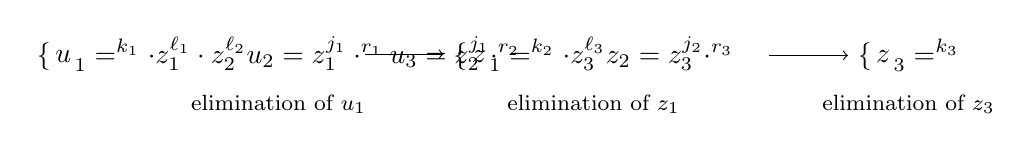
\begin{tikzpicture}
    \node[align=center] (l1) at (0,0) {
        \footnotesize{elimination of $u_1$}%\\ 
        %\footnotesize{(the fresh variables $z_1,z_2$}\\[-1pt]
        %\footnotesize{replace $u_2,u_3$)}
      };
    \node[align=center] (l2) at (4,0) {
        \footnotesize{elimination of $z_1$}%\\
        %\footnotesize{(the fresh variable $z_3$}\\[-1pt]
        %\footnotesize{replaces $z_2$)}
      };
    \node[align=center] (l3) at (8,0) {
        \footnotesize{elimination of $z_3$}%\\ 
        %~\\[-1pt]
        %~ 
      };

    \node 
      (s1) [above = 0.05cm of l1] 
      {$\begin{cases}
        u_1 = \cn^{k_1} \cdot z_1^{\ell_1} \cdot z_2^{\ell_2}\\ 
        u_2 = z_1^{j_1} \cdot \cn^{r_1}\\
        u_3 = z_2^{j_1} \cdot \cn^{r_2}
      \end{cases}$};

    \node 
      (s2) [above = 0.05cm of l2] 
      {$\begin{cases}
        z_1 = \cn^{k_2} \cdot z_3^{\ell_3}\\ 
        z_2 = z_3^{j_2} \cdot \cn^{r_3}
      \end{cases}$};

    \node 
      (s3) [above = 0.05cm of l3] 
      {$\begin{cases} 
        z_3 = \cn^{k_3}
      \end{cases}$};

    \node (t2) [left = 1cm of s2] {};
    \draw[->] (t2) -- (s2);

    \node (t3) [left = 1cm of s3] {};
    \draw[->] (t3) -- (s3);

  \end{tikzpicture}
  \vspace{-5pt}
\end{center}
We can ``backpropagate'' these substitutions to the initial variables
$u_1,\dots,u_n$, associating to each one of them an integer power of $\cn$. In the
above example, we obtain the system
\begin{center}
  $\begin{cases} u_1 = \cn^{k_1} \cdot (\cn^{k_2} \cdot
        (\cn^{k_3})^{\ell_3})^{\ell_1} \cdot ((\cn^{k_3})^{j_2} \cdot
        \cn^{r_3})^{\ell_2}\\ 
        u_2 = (\cn^{k_2} \cdot (\cn^{k_3})^{\ell_3})^{j_1} \cdot \cn^{r_1}\\
        u_3 = ((\cn^{k_3})^{j_2} \cdot \cn^{r_3})^{j_1} \cdot \cn^{r_2}
      \end{cases}$
\end{center}
By~\Cref{lemma:last-lambda-lemma,lemma:relativise-quantifiers,lemma:remove-u}, we can restrict the integers occurring 
as powers of $\cn$ in the resulting system of substitutions to a finite set.
Since the disjunction $\bigvee_i \psi_i$ is finite, 
this implies that,
under the hypothesis that $\cn$ is a computable number that is either transcendental or has a polynomial root barrier, 
it is possible to compute a finite set $P_{\phi} \subseteq \Z$ witnessing the satisfiability of $\phi$. That is, the sentence $\exists u_1\dots \exists u_n\, \phi$ is equivalent to
\[ 
  \exists u_1 \dots \exists u_n \textstyle\bigvee_{(g_1,\dots,g_n) \in (P_{\phi})^n} \textstyle\left(\phi \land \bigwedge_{i=1}^n u_i = \cn^{g_i}\right).
\]
\Cref{theorem:small-model-property} follows (in particular, the bound on $P_{\phi}$ 
for the case of $\cn$ with a polynomial root barrier is derived 
by iteratively applying the bounds in~\Cref{lemma:last-lambda-lemma,lemma:relativise-quantifiers,lemma:remove-u}).


%%% NEXT LEMMA IS NOT NEEDED ANYMORE
% \begin{restatable}{lemma}{LemmaRewritePowerPredicates}\label{lemma:rewrite-power-predicates}
%   Fix $\cn > 1$. 
%   Consider an equality $u^j = \cn^g u_1^{r_1} \cdot \ldots \cdot u_n^{r_n}$, 
%   where $g,r_1,\dots,r_n \in \Z$ and  $j \in \N$, and a pair $(m,r) \in \N$ with $m \geq 1$ and $r < m$.
%   The following formula in variables $u,u_1,\dots,u_n$ is a tautology of $\exists \R(\ipow{\cn})$:
%   \begin{equation*}
%       u^j = \cn^g u_1^{r_1} \cdot \ldots \cdot u_n^{r_n}\implies \Big(\ipowar{\cn}{m}{r}(u)\iff 
%       \bigvee_{(s_1,\dots,s_n)\in I} \ \bigwedge_{i=1}^n  \ipowar{\cn}{j \cdot m}{s_i}(u_i)\Big),
%   \end{equation*}
%   where 
%   $S \coloneqq \Big\{(s_1,\dots,s_n)\in[0..j \cdot m-1]^n : j \cdot m \text{ divides } r \cdot j - g - \sum_{i=1}^n r_i \cdot s_i\Big\}$.
% \end{restatable}

%%% PREVIOUS VERSION START OF THE SECTION
% \subparagraph*{Auxiliary notions for the procedure.}
% Following~\cite{AvigadY07},
% our procedure relies on an auxiliary function $\lambda_{\cn}
%   \colon \R_{\geq 0} \to \ipow{\cn}$ and auxiliary predicates
% $\ipowar{\cn}{m}{r}$, where $r,n \in \N$ with $r <
%   m$ and $m \geq 1$. The function~$\lambda_{\cn}$ is defined as
% $\lambda_{\cn}(0) \coloneqq 0$ and otherwise, for every $a > 0$,
% $\lambda_{\cn}(a)$ is defined as the largest integer power of $\cn$ that
% is smaller or equal than $a$, i.e., $\lambda_{\cn}(a) \leq a < \cn \cdot
%   \lambda_{\cn}(a)$. Equivalently, for $a > 0$, given the unique pair $(b,v)$
% in $\ipow{\cn} \times [1,\cn)$ such that $a = b \cdot v$, we have
% $\lambda_{\cn}(a) = b$.
% Since the number $\cn$ is fixed and not part of the input of the procedure, we
% often write $\lambda$ instead of $\lambda_{\cn}$.
% The predicate $\ipowar{\cn}{m}{r}$ is interpreted as the set
% $\{ \cn^{i \cdot m + r} : i \in \Z \}$. Note that $\ipowar{\cn}{1}{0}$ is
% equivalent
% to $\ipow{\cn}$.
% Clearly, both $\lambda$ and $\ipowar{\cn}{m}{r}$ are expressible in
% $\exists\R(\cn^{\Z})$:
% \begin{align*}
%   \lambda(x) = y  & \iff (x = 0 \land y = 0) \lor (\ipow{\cn}(y) \land y
%   \leq x < \cn \cdot y)\,;
%   \\
%   \ipowar{\cn}{m}{r}(x) & \iff \exists y : x = y^m \cdot \cn^r \land
%   \ipow{\cn}(y)\,.
% \end{align*}

% The pseudocode of our procedure is given
% in~\Cref{algo:main-procedure,algo:elim-var}. For simplicity of the
% exposition,~\Cref{algo:elim-var} is given as a non-deterministic procedure. As
% usual, a deterministic implementation can be obtained by replacing the
% non-deterministic guesses by a depth-first search (with backtracking), so that
% the overall runtime of the deterministic procedure is polynomial in the number
% of non-deterministic brances multiplied by the runtime of the non-deterministic
% procedure (a fact that we use in~\Cref{sec:complexity} for the complexity
% analysis).

% In the next two subsection, we give an overview of~\Cref{algo:main-procedure,algo:elim-var}, 
% which might be seen as a sketch of their correctness. The precise semantics of these procedures 
% is given in the specification on top of their pseudocode. Complete proofs are given in~\Cref{appendix:procedure}.

% \subsection*{Step II: solving $\exists \ipow{\cn}$}

% Let $\Cmap$ be a map from some finite set of variables to $\Z$, 
% and let $\psi$ be a formula from $\exists\R(\ipow{\cn})$, we write 
% $\psi[\cn^{\Cmap}]$ for the formula obtained from $\psi$ by replacing 
% every variable~$x$ in the domain of $\Cmap$ that occurs free in $\psi$ 
% with the constant $\cn^{\Cmap(x)}$. If this update results in polynomial inequalities featuring a negative degree (e.g., if $\Cmap(x)$ is negative)
% \am{to be continued... see text below}

% \am{todo: explain notation $\psi[\cn^{\Cmap}]$. In particular, it's the following: 
% \begin{algorithmic}
%   \For{$\omega$ in the domain of $\Cmap$}
%     \Comment{obtain a formula that is univariate in $\cn$}
%     \State update $\psi$: replace every occurrence of $\omega$ with $\cn^{\Cmap(\omega)}$
%     \EndFor
%     \State update $\psi$: replace every (in)equality $\tau \sim 0$ with $\cn^{\abs{k}} \cdot \tau \sim 0$,  where $k$ is 
%     \Statex \phantom{update $\psi$:} the largest (in absolute value) negative power of $\cn$ occurring in $\tau$
% \end{algorithmic}
% }

% Let $\vec u = (u_1,\dots,u_n)$ be a vector of variables. A formula $\phi(\vec u)$ from $\exists\R(\ipow{\cn})$ is said to be \emph{$\vec u$-typed} whenever it is of the form 
% $\gamma \land \bigwedge_{i=1}^n \ipowar{\cn}{m_i}{r_i}(u_i)$, 
% and $\gamma$ does not feature predicates~$\ipow{\cn}$. 

% \am{Essentially, $\gamma$ is from existential Tarski arithmetic enriched with the constant $\cn$.}

%%% OLD %%% 
% \begin{lemma}
%   Consider $\phi(u,\vec y)$ a quantifier-free formula from $\exists \R(\ipow{\cn})$, 
%   and let $u$ be a variable from $\vec u$. 
%   The following formula is a tautology of $\exists \R(\ipow{\cn})$: 
%   \begin{equation*}
%     (\exists u\, \phi)
%     \iff 
%     \bigvee_{\ell \in [-m,m]}\ 
%     \bigvee_{q \in Q}\ 
%     \bigvee_{(\mu,g,\vec y^{\vec \ell_1}, \vec y^{\vec \ell_2}) \in F_q}
%     \exists u \left( \vec y^{\vec \ell_1} \cdot u^{\mu} = \cn^{\mu \cdot \ell + g} \cdot \vec y^{\vec \ell_2} \land \phi \right),
%   \end{equation*}
%   where
%   \begin{itemize}
%     \item the integer $m \geq 1$ is such that $\ipowar{\cn}{m}{r}(u)$ occurs in $\phi$, for some $r \in \N$, \am{in new version, this might not be required.}
%     \item the set $Q$ contains the polynomial $u-1$ as well as all polynomials in $\phi$ featuring $u$,
%     \item given $q \in Q$, $F_q$ is the finite set obtained by applying~\Cref{lemma:last-lambda-lemma}
%     to $r(x,v,\vec y) \coloneqq q\sub{x \cdot v}{u}$, where $x$ and $v$ 
%     are two fresh variables.
%   \end{itemize}
% \end{lemma}
\section{Proof of Theorem~\ref{theorem:result-root-barrier}: classical numbers with polynomial root barriers}\label{sec:poly-evaluation}

In this section, we complete the proof of~\Cref{theorem:result-root-barrier} by
establishing~\Cref{theorem:result-root-barrier}.\ref{theorem:result-root-barrier:point1}
and~\Cref{theorem:result-root-barrier}.\ref{theorem:result-root-barrier:point2}.
Following~\Cref{theorem:general-result-root-barrier}, we discuss natural choices for the base $\cn > 0$ that \textbf{(i)} can be computed with
polynomial-time Turing machines and \textbf{(ii)} have polynomial root barriers. 


\subparagraph*{The case of~$\cn$ algebraic.} 
Let $\cn$ be a fixed algebraic number represented by $(q,\ell,u)$.
The following two results (the first one based on performing a dichotomy search 
to refine the interval~$[\ell,u]$) 
show that one can construct a polynomial-time Turing machine for $\cn$, 
and that~$\cn$ has a polynomial root barrier where the integer~$k$ from~\Cref{theorem:general-result-root-barrier} equals $1$.

\begin{restatable}{lemma}{LemmaApproxAlgebraicBody}
  \label{lemma:approx-algebraic-body}
  Given an algebraic number~$\alg$ represented by $(q,\ell,u)$, 
  one can construct a polynomial-time Turing machine computing $\alg$.
\end{restatable}

\vspace{-7pt}

\begin{restatable}[{\cite[Theorem~A.1]{Bugeaud04}}]{theorem}{TheoremAlgRootBarrier}\label{theorem:alg-root-barrier}
  Let $\alg \in \R$ be a zero
  of a non-zero integer polynomial~$q(x)$,
  and consider a non-constant integer polynomial $p(x)$.
  Then, either ${p(\alg) = 0}$ or 
  ${\ln \abs{p(\alg)} \geq - \deg(q) \cdot \big(\ln(\deg(p)+1) + \ln \height(p)\big)
  - \deg(p) \cdot \big( \ln(\deg(q)+1) + \ln \height(q) \big)}$.
\end{restatable}

By applying~\Cref{theorem:general-result-root-barrier}.\ref{theorem:general-result-root-barrier:point1}, 
\Cref{lemma:approx-algebraic-body} and~\Cref{theorem:alg-root-barrier}, we deduce that the satisfiability problem for $\exists\R(\ipow{\cn})$ is in \twoexptime. However, for algebraic numbers it is possible to obtain a better complexity result (\expspace) by slightly modifying~Steps~II and~III of~\Cref{algo:main-procedure}.

\begin{proof}[Proof of~\Cref{theorem:result-root-barrier}.\ref{theorem:result-root-barrier:point1}]
Let $\phi$ be a formula in input of~\Cref{algo:main-procedure}, and
$\psi(u_1,\dots,u_n)$ to be the formula obtained from $\phi$ after executing
lines~\ref{algo:line1}--\ref{algo:line6}. In lines~\ref{algo:line7}
and~\ref{algo:line8}, guess the integers~$g_1,\dots,g_n$ in binary, instead of
unary. These numbers have at most $m$ bits where,
by~\Cref{theorem:basu,theorem:small-model-property}, $m$ is exponential
in~$\size(\phi)$. Let $g_i = \pm_{i} \sum_{j=0}^{m-1} d_{i,j} 2^j$, with
$d_{i,j} \in \{0,1\}$ and $\pm_i \in \{+1,-1\}$, so that $\cn^{g_i} =
\prod_{j=0}^{m-1}\cn^{\pm_i d_{ij}2^j}$. Note that the formula 
\[ 
  \gamma(x_0,\dots,x_{m-1}) \coloneqq q(x_0) = 0 \land \ell \leq x_0 \leq u \land \textstyle\bigwedge_{i=1}^{m-1} x_i = (x_{i-1})^2
\]
has a unique solution: for every $j \in [0..m-1]$, $x_j$ must be equal to
$\cn^{2^j}$. The formula $\psi$ is therefore equisatisfiable with the formula
$\psi' \coloneqq \psi\sub{x_0}{\cn} \land \gamma \land \bigwedge_{i=1}^n u_i =
\prod_{j=0}^{m-1}x_j^{\pm_id_{ij}}$, which (after rewriting $u_i =
\prod_{j=0}^{m-1}x_j^{\pm_id_{ij}}$ into $u_i \prod_{j=0}^{m-1}x_j^{d_{ij}} = 1$
when $\pm_i = -1$) is a formula from the existential theory of the reals of size
exponential in $\size(\phi)$. Since the
satisfiability problem for the existential theory of the reals is in
\pspace~\cite{Canny88}, we conclude that checking whether $\psi'$ is satisfiable
can be done in~\expspace. Accounting for Steps I and II, we thus obtain a
procedure running in non-deterministic exponential space (because of the guesses
in lines~\ref{algo:line7} and~\ref{algo:line8}), which can be determinised by
Savitch's theorem~\cite{Savitch70}.
%This concludes the proof of~\Cref{theorem:result-root-barrier}.\ref{theorem:result-root-barrier:point1}.
\end{proof}

\subparagraph*{The case of $\cn$ among some classical transcendental numbers (proof sketch of~\Cref{theorem:result-root-barrier}.\ref{theorem:result-root-barrier:point2}).}%
In the context of transcendental numbers, root barriers are usually called
\emph{transcendence measures}. Several fundamental results in number theory
concern deriving a transcendence measure for ``illustrious'' numbers, such as
Euler's $e$, $\pi$, or logarithms of algebraic
numbers~\cite{Popken29,Mahler32,Waldschmidt78}. A few of these results are
summarised in~\Cref{table:transcendence-degrees}, which is taken almost verbatim
from~\cite[Fig.~1 and Corollary~4.2]{Waldschmidt78}. All transcendence
measures in the table are \emph{polynomial} root barriers. Note that in the cases of
$\alg^\eta$ and $\frac{\ln \alg}{\ln \beta}$, the transcendence measures hold
under further assumptions, which are given in the caption of the table.
\begin{table} 
  \begin{center}
  \def\arraystretch{1.15}
    \begin{tabular}{c|l|l}
      Number & \hfill Transcendence measure from~\cite{Waldschmidt78} & \hfill Simplified bound ($\alg,\beta,\eta$ fixed)\\[2pt]
      \hline
      \rule{0pt}{1.1\normalbaselineskip}
      $\pi$ & $2^{40} d (\ln h + d \ln d)(1 + \ln d)$
      & $O(d^2 (\ln d)^2 \ln h)$\\
      $e^\pi$ & $2^{60} d^2 (\ln h + \ln d)(\ln \ln h + \ln d)(1 + \ln d)$
      & $O(d^2 (\ln d)^3 (\ln h) (\ln \ln h))$\\
      $e^\eta$ & $c_\eta \cdot d^2(\ln h + \ln d)\big(\frac{\ln \ln h + \ln d}{\ln \ln h + \ln \max(1,\ln d)}\big)^2$
      & $O(d^2 (\ln d)^3 (\ln h)(\ln \ln h)^2)$\\ 
      $\alg^\eta$ 
      & $c_{\alg,\eta} \cdot d^3 (\ln h + \ln d)\frac{\ln \ln h + \ln d}{(1+\ln d)^2}$
      & $O(d^3 (\ln d)^2(\ln h)(\ln \ln h))$\\
      $\ln \alg$ & $c_\alg \cdot d^2 \frac{\ln h + d \ln d}{1+\ln d}$ & $O(d^3 (\ln d) \ln h)$\\ 
      $\frac{\ln \alg}{\ln \beta}$ 
      & $c_{\alg,\beta} \cdot d^3 \frac{\ln h + d \ln d}{(1+\ln d)^2}$
      & $O(d^4 (\ln d) \ln h)$\\
    \end{tabular}
    \vspace{-4pt}
  \end{center}
\caption{Transcendence measures for some classical real numbers. 
For convenience only, the table assumes $h \geq 16$ (so that $\ln \ln h \geq 1$; replace $h$ by $h+15$ to avoid this assumption).
The numbers $\alg > 0$, $\beta > 0$ and $\eta$ are fixed algebraic numbers, with $\beta \neq 1$.
The integers $c_{\eta}$, $c_{\alg,\eta}$, $c_{\alg}$ and $c_{\alg,\beta}$ are constants that depend on, and can be computed from, polynomials representing $\alg$, $\beta$ and $\eta$.
In the case of $\alg^\eta$, $\eta$ is assumed to be irrational.
In the last line of the table, $\frac{\ln \alpha}{\ln \beta}$ is assumed to be irrational.\vspace{-2pt}}%
\label{table:transcendence-degrees}%
\end{table}

Following~\Cref{theorem:general-result-root-barrier}.\ref{theorem:general-result-root-barrier:point2},
to
prove~\Cref{theorem:result-root-barrier}.\ref{theorem:result-root-barrier:point2}
it suffices to show how to construct a polynomial-time Turing machine for every
number in~\Cref{table:transcendence-degrees}, and derive polynomial root
barriers for the cases $\cn = \alg^{\eta}$ and $\cn = \frac{\ln{\alg}}{\ln
\beta}$ without relying on the additional assumptions in the table. The
following two results solve the first of these two issues.

\begin{theorem}[\cite{Bailey1997OnTR}]\label{lemma:poly-time-pi}
  One can construct a polynomial-time Turing machine computing $\pi$.
\end{theorem}

\vspace{-5pt}

\begin{restatable}{lemma}{LemmaPolyTimeTMExpLog}
  \label{lemma:poly-time-exp-log}
  Given a polynomial-time Turing machine computing $r \in \R$,
  \begin{enumerate}
    \item\label{lemma:poly-time-exp-log:point1} one can construct a polynomial-time Turing machine computing $e^r$;
    \item\label{lemma:poly-time-exp-log:point2} if $r > 0$, one can construct a polynomial-time Turing machine computing $\ln(r)$.
  \end{enumerate}

\end{restatable}

\begin{proof}[Proof idea]
  The two Turing machines use the power series in the
  identities $e^x = \sum_{j=0}^\infty \frac{x^j}{j!}$ and $\ln(x) = 2
  \sum_{j=0}^\infty \big(\frac{1}{2j+1} \big(\frac{x-1}{x+1}\big)^{2j+1}\big)$,
  truncated to obtain the required accuracy. 
\end{proof}

As an example, to construct the Turing machine for~$\frac{\ln(\alg)}{\ln(\beta)}$ 
we construct machines for the following sequence of numbers: $\alg$ and $\beta$ (applying~\Cref{lemma:approx-algebraic-body}), $\ln(\alg)$ and $\ln(\beta)$ (\Cref{lemma:poly-time-exp-log}.\ref{lemma:poly-time-exp-log:point2}), $\frac{1}{\ln(\beta)}$ (\Cref{lemma:turing-machine-reciprocal})
and $\frac{1}{\ln(\beta)} \cdot \ln(\alg)$ (\Cref{lemma:turing-machine-products}). 
For $\alg^\eta$, we follow the operations in $e^{\eta \cdot \ln(\alg)}$.


Let us now discuss how to derive polynomial root barriers when $\cn = \alg^\eta$
or $\cn = \frac{\ln(\alg)}{\ln(\beta)}$. In~the~case~$\cn = \alg^\eta$,
\Cref{table:transcendence-degrees} assumes~$\eta$ to be irrational. To check
whether an algebraic number represented by~$(q,\ell,u)$ is rational, it suffices
to factor $q(x)$ into a product of irreducible polynomials with rational
coefficients, and test for any degree $1$ factor $n \cdot x - m$ whether the
rational number $\frac{m}{n}$ belongs to $[\ell,u]$. The factorisation of $q$
can be computed (in fact, in polynomial time) using LLL~\cite{lenstra1982}. If
such a rational number does not exist, then $\eta$ is irrational and
the polynomial root barrier for $\alg^\eta$ is given
in~\Cref{table:transcendence-degrees}. Otherwise, $\eta = \frac{m}{n}$ and the
number $\alg^{\frac{m}{n}}$ is algebraic. In this case, rely on the following
lemma to construct a representation of $\alg^{\frac{m}{n}}$, and then derive a
polynomial root barrier by applying~\Cref{theorem:alg-root-barrier}.

\begin{restatable}{lemma}{LemmaRepresentationPowerOfAlgebraic}
  \label{lemma:representation-power-of-algebraic}
  There is an algorithm that given a rational $r$ and an algebraic number $\alg > 0$ 
  represented by $(q,\ell,u)$, computes a representation $(q',\ell',u')$ 
  of the algebraic number $\alg^r$.
\end{restatable}

We move to the case $\cn = \frac{\ln(\alg)}{\ln(\beta)}$,
which~\Cref{table:transcendence-degrees} assumes to be irrational. Since $\cn$
is positive, $\alg,\beta \not\in \{0,1\}$. We observe that for every
$\frac{m}{n} \in \Q$, we have $\cn = \frac{m}{n}$ if
and only if~${\alg^n \beta^{-m} = 1}$. (In other words,
$\frac{\ln(\alg)}{\ln(\beta)} \in \Q$ if and only if $\alg$ and $\beta$ are
multiplicatively dependent.) From a celebrated result of Masser~\cite{Masser88},
the set $\{(m,n) \in \Z^2 : \alg^n \beta^{-m} = 1\}$ is a
finitely-generated integer lattice for which we can explicitly construct a
basis~$K$ (see~\cite{CaiLZ00} for a polynomial-time procedure). If $K =
\{(0,0)\}$, then $\cn$ is irrational and its polynomial
root barrier is given in~\Cref{table:transcendence-degrees}. Otherwise, since
$\alg,\beta \not \in \{0,1\}$, there is~$(m,n) \in K$ with $n \neq 0$, and
$\cn = \frac{m}{n}$. We can then derive a polynomial
root barrier by applying~\Cref{theorem:alg-root-barrier}.

% \begin{theorem}[\cite{CaiLZ00}]\label{theorem:multiplicative-idependence}
%   There is an algorithm that given as input algebraic numbers $\alg_1,\dots,\alg_n$, 
%   returns a basis for the lattice $\{(d_1,\dots,d_n) \in \Z^n : \alg_1^{d_1} \cdot \ldots \cdot \alg_n^{d_n} = 1\}$.
% \end{theorem}




%%%%%%%%%%%%%%%%%%%%%%%%%%%%%%%%%%%%%%%%%%%
%%%%%% OLD MATERIAL COMMENTED BELOW 
%%%%%%%%%%%%%%%%%%%%%%%%%%%%%%%%%%%%%%%%%%%
% \subparagraph*{The case of $\cn=\alg^\beta$.}
% Let $\cn$ be $\alpha^\beta$ where both $\alpha$ and $\beta$ are algebraic. 
% %Observe that in \Cref{table:transcendence-degrees}, $\alpha\neq 0$, $1$, and 
% %$\beta$ is assumed to be irrational in this case. This is because 
% %$\alpha^\beta$ is algebraic if and only if $\beta$ is rational.
% Excluding the trivial cases where $\alg\in\{0,1\}$ or $\beta=0$,
% there are two subcases depending on the rationality of $\beta$. 
% This can always be checked from the representation of $\beta$ as 
% an algebraic number thanks to the next result.


% %\am{If you want, I have used a trick in~\Cref{sec:application-entropic-risk} that might help here. Briefly, when dealing with a term $x^{\frac{p}{q}}$, you can introduce a variable~$y$, write $y^q = x$ and replace $x^{\frac{p}{q}}$ with $y^p$.}

% %\jg{text below to be moved to the appendix in case this method is used}
% %Consider $\beta=b_1/b_2$ a rational number and
% %$\alpha$ the only root of the polynomial $p(x)=\sum_{i=0}^da_ix^i$ in 
% %the interval $(l,u)$. The following is a way to compute a polynomial 
% %that has $\alpha^\beta$ as a root.
% %The fact that $\alpha$ is a root of a polynomial of degree $d$, implies
% %that every power of $\alpha$ can be written as a linear combination of 
% %terms $r\cdot \alpha^j$, where $r$ is a rational number and $j\in[0..d-1]$.
% %
% %Therefore we can build a matrix of $d$ columns where in each row
% %we have the coefficients of the rational linear combinations equal to 
% %$(\alpha^b)^k$ with $k\in[0..d]$.

% The following result is useful when $\beta$ is irrational.


% If $\beta$ is irrational then $\cn$ has the root barrier from 
% \Cref{table:transcendence-degrees} corresponding to $\alg^\beta$. 
% Let us show that $\cn$ is computable by a polynomial-time Turing machine
% so that we can apply \Cref{theorem:general-result-root-barrier}.

% We write $\alg^\beta$ as $e^{\ln(\alg)\beta}$. By \Cref{lemma:approx-algebraic}
% we can construct two different polynomial-time Turing machines that compute $\alg$
% and $\beta$, by \Cref{lemma:turing-machine-products} we can also construct
% a polynomial-time Turing machine that computes $\ln(\alg)\cdot\beta$ and 
% finally applying \Cref{lemma:poly-time-exp-log} we deduce that we can construct
% a polynomial-time Turing machine that computes $e^{\ln(\alg)\beta}=\alg^\beta$. 

% Therefore considering the polynomial
% root barrier from \Cref{table:transcendence-degrees} related to $\alg^\beta$ 
% we can apply \Cref{theorem:general-result-root-barrier}.\ref{theorem:general-result-root-barrier:point2},
% \Cref{lemma:approx-algebraic}, \Cref{lemma:poly-time-exp-log} and 
% \Cref{lemma:turing-machine-products} in the way described to 
% deduce that the satisfiability problem for $\exists\R(\ipow{\cn})$ is in \threeexptime.


% \subparagraph*{The case of $\cn=\frac{\ln(\alg)}{\ln(\beta)}$.} 
% Let $\cn$ be $\frac{\ln(\alg)}{\ln(\beta)}$ where both $\alg$ and $\beta$
% are algebraic, non-zero and different from 1. In order to apply the root barrier from \Cref{table:transcendence-degrees}
% we have to check rationality of $\cn$. 
% This can be done studying the multiplicative dependence of 
% $\alpha$ and $\beta$, that is, whether they satisfy $\alpha^n=\beta^m$ 
% for some non-zero integers $n$, $m$. The following lemma allows this.


% Therefore applying \Cref{theorem:multiplicative-idependence} and 
% \Cref{lemma:mult-independence-rationality} we can decide the rationality 
% of $\cn$. 

% If $\cn$ is rational,
% algorithm from \Cref{theorem:multiplicative-idependence} 
% returns some integers $n$ and $m$ such that $\alpha^n=\beta^m$,hence 
% $\cn=\frac{m}{n}$
% and we can proceed as in the case 
% of $\cn$ algebraic. A representation 
% of $\cn$ as an algebraic number is given by $q(x)=n\cdot x-m$, 
% $l=\frac{m}{n}-1$ and $u=\frac{m}{n}+1$. 

% If on the other hand $\cn$ is irrational we proceed as follows. Since $\cn>0$, 
% in this case this means that either both $\alpha$, $\beta>1$ or both 
% $\alpha$, $\beta\in(0,1)$. When one of these conditions holds, something
% that can be checked in constant time, 
% $\cn=\frac{\ln(\alg)}{\ln(\beta)}=\frac{\abs{\ln(\alg)}}{\abs{\ln(\beta)}}$.
% From the previous subsections we know that $\ln(\alg)$ and $\ln(\beta)$
% can be computed by polynomial-time Turing machines and 
% since we know their sign, also can 
% $\abs{\ln(\alg)}$ and $\abs{\ln(\beta)}$. 
% From \Cref{lemma:turing-machine-reciprocal} we deduce
% that $\frac{1}{\abs{\ln(\beta)}}$ can also be computed by a polynomial-time
% Turing machine and finally by \Cref{lemma:turing-machine-products} the 
% same holds for $\abs{\ln(\alg)}\cdot \frac{1}{\abs{\ln(\beta)}}$.
% From \Cref{table:transcendence-degrees} we have a polynomial root 
% barrier for $\cn$.

% Therefore we can apply 
% \Cref{theorem:general-result-root-barrier}.\ref{theorem:general-result-root-barrier:point2} 
% to deduce that the satisfiability problem 
% for $\exists\R(\ipow{\cn})$ is in \threeexptime.


% \am{Shall we take the exact bounds from \cite{CaiLZ00}, and give a result for the root barrier of $\frac{\ln(\alg)}{\ln(\beta)}$ that does not ask for irrationality?}
%\input{sec-complexity}
\section{Application on Medical QA}


\section{Conclusion and Discussion}
\label{sec:conclusion}

We introduce a novel framework for augmenting \emph{any} lossy compressor to preserve the contour tree of a volumetric dataset while maintaining a user-specified global error bound. 
To do this, our framework first imposes topology-informed upper and lower bounds on each data point. 
It then progressively tightens those bounds until the contour tree is preserved. 
We also introduce a novel encoding scheme that efficiently stores individual points with variable precision and maintains these upper and lower bounds. 
When our framework is used to augment state-of-the-art lossy compressors, it is shown to preserve the contour trees of various scientific datasets.
Our augmented compressors also achieve higher compression ratios and reconstruction quality than those obtained by existing topology-preserving compressors in comparable or faster time.
Our framework will benefit from any advancement with lossy compression since it can be used to augment increasingly effective lossy compressors to achieve better topology-preserving compression. 

Our framework is not without limitations. The compression times are longer than the base compressors. This difference gets worse as the topological complexity of the data increases.
However, in some use-cases, topological preservation is preferable to run time.
Regardless, our framework would benefit from more efficient or parallel implementations for the contour/merge tree computation and the encoding scheme. 


%%
%% Bibliography
%%

\bibliography{bibliography}

%%
%% Appendix
%%

\newpage
\appendix
\allowdisplaybreaks
\section{Proofs of the statements in Section~\ref{sec:preliminaries}}
\label{appendix:preliminaries}

\LemmaTuringMachineProducts*

\begin{proof}
Let $\ell \coloneqq \ceil{\log(\abs{T_0}+\abs{T_0'}+3)}$.
We define $T''$ as the Turing machine that on input $n$ returns the 
rational number $T_{n+\ell} \cdot T_{n+\ell}'$. 
Clearly, $T''$ runs in time polynomial in $n$.
We show that $\abs{a \cdot b - T''} \leq \frac{1}{2^n}$ for every $n \in \N$, 
i.e., $T''$ computes $a \cdot b$. 
Let $\epsilon_1 \coloneqq T_{n+\ell}-a$ and $\epsilon_2 \coloneqq T_{n+\ell}'-b$. Recall that $\abs{\epsilon_1},\abs{\epsilon_2} \leq \frac{1}{2^{n+\ell}}$. 
Then, 
\begin{align*}
  \abs{a \cdot b - T''} &=
  \abs{a \cdot b - T_{n+\ell} \cdot T_{n+\ell}'} =
  \abs{a \cdot b - (a+\epsilon_1) \cdot (b+\epsilon_2)}\\
  &=\abs{a \cdot \epsilon_2 + b \cdot \epsilon_1 + \epsilon_1 \cdot \epsilon_2}\\
  &\leq \abs{a} \cdot \abs{\epsilon_2} + \abs{b} \cdot \abs{\epsilon_1} + \abs{\epsilon_1} \cdot \abs{\epsilon_2}\\
  &< \frac{\abs{a}+\abs{b}+1}{2^{n+\ell}}
  &\text{since} \abs{\epsilon_1},\abs{\epsilon_2} \leq \frac{1}{2^{n+\ell}}\\
  &= \frac{\abs{a}+\abs{b}+1}{2^{n+\ceil{\log(\abs{T_0}+\abs{T_0'}+3)}}}
  &\text{def.~of~$\ell$}\\
  &\leq \frac{1}{2^{n}}\frac{\abs{a}+\abs{b}+1}{\abs{T_0}+\abs{T_0'}+3}\\
  &\leq \frac{1}{2^{n}}\frac{\abs{a}+\abs{b}+1}{\abs{a}+\abs{b}+1}
  &\hspace{-2.4cm}\text{since $\abs{a} \leq \abs{T_0}+1$ and $\abs{b} \leq \abs{T_0'}+1$}\\
  &\leq \frac{1}{2^n}
  &&\qedhere
\end{align*}
\end{proof}

\LemmaTuringMachineReciprocal* 

\begin{proof}
  Compute the smallest $k \geq 2$ such that
  $\frac{1}{2^k} < \abs{T_k}$; its existence follows from the fact
  that $\lim_{n \to \infty} T_n = r \neq 0$, whereas $\lim_{n \to \infty}
  \frac{1}{2^n} = 0$. Since $\abs{r - T_k} \leq \frac{1}{2^k}$, we have 
  that and $T_k$ and $r$ have the same sign, and $0 < \abs{T_k}-\frac{1}{2^k} \leq \abs{r}$. 
  Let $T_k = \frac{p}{q}$, where $p \in \Z \setminus \{0\}$ and $q \geq 1$, 
  and define ${\ell \coloneqq 2(k + \ceil{\log(q)})}$.

  For the time being, let us give a construction of $T'$ that depends on the sign of $T_k$.

  \begin{description}
    \item[case: $T_k > 0$.] 
      We define $T'$ as the Turing machine that on input $n$ returns the
      rational $\frac{1}{\max(\abs{T_{n+\ell}},T_k - 2^{-k})}$. Clearly, if $T$
      runs in time polynomial in $n$, so does $T'$. We
      prove that $T'$ computes~$\frac{1}{r}$. First, observe that
      $\abs{r-T_{n+\ell}} \leq \frac{1}{2^{n+\ell}}$ and $r > 0$ imply
      $\abs{r-\abs{T_{n+\ell}}} \leq \frac{1}{2^{n+\ell}}$. Then, because $0 <
      T_k - 2^k \leq r$, we have $\abs{r-\max(\abs{T_{n+\ell}},T_{k}-2^{-k})}
      \leq \frac{1}{2^{n+\ell}}$.

      For
      every $n \in \N$,
      \begin{align*}
        \abs{\frac{1}{r} - T_n'}
        &= \abs{\frac{r - \max(\abs{T_{n+\ell}},T_{k}-2^{-k})}{r \cdot \max(\abs{T_{n+\ell}},T_{k}-2^{-k})}}\\
        &\leq \frac{1}{2^{n+\ell}} 
        \cdot \frac{1}{r \cdot \max(\abs{T_{n+\ell}},T_{k}-2^{-k})}\\
        &\leq \frac{1}{2^{n+\ell} \cdot (T_k-2^{-k})^2}
        &\text{since } 0 < T_k - 2^{-k} \leq r\\
        &\leq \frac{1}{2^{n+\ell+2\log(T_k - 2^{-k})}}
      \end{align*}
      To conclude the proof it suffices to show $\ell + 2\log(T_k-2^{-k}) \geq 0$:
      \begin{align*}
        & \ell + 2\log(T_k-2^{-k})\\
        ={}& \ell + 2\log((2^{k}T_k-1)2^{-k})
        = \ell + 2\log\Big(\Big(\frac{2^{k}p-q}{q}\Big)2^{-k}\Big)\\
        ={}& \ell + 2\log(2^{k}p-q) -2\log(q) -2k\\
        \geq{}& \ell -2\log(q) -2k 
        & \text{since $2^kp-q$ is an integer,}\\
        && \hspace{-1.8cm}\text{from $\frac{1}{2^k} < T_k$ we get $\log(2^{k}p-q) \geq 0$}\\
        ={}& 2(k+\ceil{\log(q)}-\log(q)-k)
        &\text{by def.~of~$\ell$}\\
        \geq{}& 0.
      \end{align*}
    \item[case: $T_k < 0$.] 
      Since $\abs{r}$ is computed by the machine that on input $n$ returns $\abs{T_n}$, 
      by following the previous case of the proof
      we conclude that $\frac{1}{\abs{r}}$ 
      is computed by the Turing machine that on input $n$
      returns the positive rational $\frac{1}{\max(\abs{T_{n+\ell}},\abs{T_k} - 2^{-k})}$.
      Then, the Turing machine that on input $n$
      returns the negative rational $\frac{-1}{\max(\abs{T_{n+\ell}},\abs{T_k} - 2^{-k})}$
      computes $\frac{1}{r}$.
  \end{description}
  Putting the two cases together we conclude that $\frac{1}{r}$ 
  is computed by the Turing machine 
  that on input $n$ returns the non-zero rational number $\frac{s}{\max(\abs{T_{n+\ell}},\abs{T_k} - 2^{-k})}$, 
  where $s = +1$ if $T_k > 0$, and otherwise $s = -1$.
\end{proof}


\section{Proofs of the statements in Section~\ref{sec:the-algorithm} (except for Proposition~\ref{theorem:small-model-property} which is proven in Appendix~\ref{appendix:solving-substructure}) and proof of Theorem~\ref{theorem:general-result-root-barrier}}
\label{appendix:useful-lemmas}

\begin{restatable}{lemma}{LemmaApproxUnivPolynomial}
  \label{lemma:approx-univ-polynomial}
  Let $p(x)$ be an integer polynomial, 
  and let ${r \in \R}$ with $\abs{r} \leq K$ for some $K \geq 1$.
  Consider $L,M \in \N$ satisfying 
  $M\geq L + \log(\height(p)+1) + 2 \deg(p) \cdot \log(K+1)$.
  For every $r^* \in \R$, if $\abs{r-r^*} \leq 2^{-M}$, 
  then $\abs{p(r)-p(r^*)} \leq 2^{-L}$.
\end{restatable}

\begin{proof} 
  Let $p(x) \coloneqq \sum_{j=0}^d a_i \cdot x^j$, and
  suppose $\abs{r-r^*} \leq 2^{-M}$.
  If $d = 0$, then $p$ is a constant polynomial and $\abs{p(r)-p(r^*)} = 0$, 
  which proves the lemma. 
  Below, we assume $d \geq 1$.

  To show that $\abs{p(r)-p(r^*)} \leq 2^{-L}$, let us start by bounding the maximum of the absolute value
  that the first derivative $p'(x) = \sum_{j=1}^d a_j \cdot j \cdot x^{j-1}$ of
  $p$ takes in the interval $I \coloneqq [-(K+1),K+1]$. For every $x \in \R$, $\abs{p'(x)} \leq
  g(x) \coloneqq \sum_{j=1}^d \abs{a_j \cdot j \cdot x^{j-1}}$. Since the
  function $g$ is monotonous over $\R_{\geq 0}$, and $g(y) = g(-y)$ for every $y
  \in \R$, we conclude that for every $x \in I$, $\abs{p'(x)} \leq g(K+1) =
  \sum_{j=1}^d \abs{a_j} \cdot j \cdot (K+1)^{j-1} \leq d^2 \height(p) (K+1)^{d-1}$. 
  
  From $\abs{r} \leq K$ and $\abs{r-r^*} \leq 2^{-M}$, where $M \geq 0$, 
  we have that both $r$ and $r^*$ belong to~$I$.
  This implies $\frac{\abs{p(r) -
  p(r^*)}}{\abs{r-r^*}} \leq \max\{\abs{p'(x)} : x \in I \} \leq
  d^2 \height(p) (K+1)^{d-1}$. So,
  \begin{align*}
    & \abs{p(r) - p(r^*)}\\
    \leq{}& d^2 \height(p) (K+1)^{d-1} \abs{r-r^*}\\
    \leq{}& 2^{2 \log(d)} 2^{\log(\height(p))} 2^{(d-1)\log(K+1)} 2^{-M}
    \\
    \leq{}& 2^{2 \log(d)+\log(\height(p))+(d-1)\log(K+1)-(L + \log(\height(p)+1) + 2 d \cdot \log(K+1))}
    & \text{bound on $M$}\\
    \leq{}& 2^{2 \log(d)-L-(d+1) \cdot \log(K+1)}\\
    \leq{}& 2^{-L}.
    &\hspace{-4.5cm}\text{since $2 \log(d) \leq d$ and $\log(K+1) \geq 1$}&\qedhere
  \end{align*}
\end{proof}

\LemmaSignPolyRootBarrier*

\begin{proof}
  Let $p(x) = \sum_{j=0}^d a_j \cdot x^j$ be input integer polynomial, having
  degree $d = \deg(p) \geq 1$ and height $h = \height(p)$. Recall that, from the
  definition of root barrier, whenever $p(\cn) \neq 0$ we have $\abs{p(\cn)}
  \geq e^{-\sigma(d,h)} > 2^{-2 \sigma(d,h)}$, where the last inequality
  follows from $\sigma(d,h) \geq 0$. Following
  line~\ref{algo:sign-evaluation:bound-on-n}, define $n \coloneqq 1 +
  2 \sigma(d,h) + 3d\ceil{\log(h+4)}$. 
  Note that $n \geq 5$.

  Let us first assume that $\abs{T_n} \geq h + 2$. In this case, the algorithm
  returns the sign of $p(T_n)$ (line~\ref{algo:sign-evaluation:large-pTn}). We
  show that $p(T_n)$ and $p(\cn)$ have the same sign. Since $\abs{\cn-T_n}
  \leq 2^{-1}$, we have $\abs{\cn} > h+1$.  
  By a result of Cauchy~\cite[Chapter 8]{Rahman02}, $h+1$ is an upper bound to
  the absolute value of every root of $p$. This implies that there are no root
  of $p$ in the interval $[\cn,T_n]$, so in particular $\cn$ and $T_n$ are
  not roots of $p$, and $p(\cn)$ and $p(T_n)$ have the same sign.
  
  Let us consider now the case $\abs{T_n} < h + 2$, and so $\abs{\cn} \leq K
  \coloneqq h + 3$. From the definition of $n$ and the fact that $\abs{\cn-T_n}
  \leq 2^{-n}$, by~\Cref{lemma:approx-univ-polynomial} we conclude that
  $\abs{p(\cn) - p(T_n)} \leq 2^{-2 \sigma(d,h)-1}$. This implies that if
  $\abs{p(T_n)} \leq 2^{-2 \sigma(d,h)-1}$ then $p(\cn) = 0$, and
  otherwise $p(T_n)$ and $p(\cn)$ have the same sign;  
  which concludes the proof of the lemma (see
  lines~\ref{algo:sign-evaluation:small-pTn}
  and~\ref{algo:sign-evaluation:large-pTn}). Indeed,  
  \begin{itemize}
    \item If $p(\cn) = 0$ then $\abs{p(T_n)} \leq 2^{-2 \sigma(d,h)-1}$
    (from $\abs{p(\cn) - p(T_n)} \leq 2^{-2 \sigma(d,h)-1}$).
    \item If $p(\cn) \neq 0$, then $\abs{p(T_n)} > 2^{-2 \sigma(d,h)-1}$
    :
    \begin{align*}
      \abs{p(T_n)} 
      & \geq \abs{p(\cn)} - \abs{p(\cn) - p(T_n)}
      & \text{from properties of the absolute value}\\
      & > 2^{-2 \sigma(d,h)} - 2^{-2 \sigma(d,h)-1}
      & \text{bounds on $\abs{p(\cn)}$ and $\abs{p(\cn) - p(T_n)}$}\\
      & = 2^{-2 \sigma(d,h)-1}.
    \end{align*}
    Moreover, $\abs{p(\cn) - p(T_n)} \leq 2^{-2 \sigma(d,h)-1}$ and
    $\abs{p(T_n)} > 2^{-2 \sigma(d,h)-1}$ imply that $p(\cn) > 0$ if and
    only if $p(T_n) > 0$.
    \qedhere
  \end{itemize}
\end{proof}

\LemmaRuntimeSignPolyRootBarrier* 

\begin{proof}
  When encoded in unary, the number $n$ defined in
  line~\ref{algo:sign-evaluation:bound-on-n} has size polynomial in the size of
  the input polynomial $p$. Then, to compute $T_n$ only requires polynomial time
  in $\size(p)$. Observe that this implies $T_n = \frac{q}{d}$ for some integers
  $q$ and $d$ encoded in binary using polynomially many bits with respect to $\size(p)$. Evaluating a
  polynomial at such a rational point can be done in polynomial time in the size of
  the polynomial and of the bit size of the rational. 
  This means that also lines~\ref{algo:sign-evaluation:small-pTn}
  and~\ref{algo:sign-evaluation:large-pTn} run in polynomial time in $\size(p)$.
\end{proof}

\LemmaCorrectnessAlgorithmOne* 

\begin{proof}
  Consider an input
  formula $\phi(x_1,\dots,x_n)$, and let $\phi'(u_1,\dots,u_n,v_1,\dots,v_n)$ be
  the formula obtained from it at the completion of the \textbf{for} loop of
  line~\Cref{algo:line1}. Note that if $\phi$ and $\phi'$ are equisatisfiable,
  then the lemma follows. Indeed, 
  \begin{itemize}
    \item By~\Cref{theorem:basu}, the formula $\psi(u_1,\dots,u_n)$ in
    line~\ref{algo:line6} is equisatisfiable with $\phi'$,
    \item By~\Cref{theorem:small-model-property}, $\psi$ is satisfiable if and
    only if it has a solution from the set $S = \{(\cn^{j_1},\dots,\cn^{j_n}) :
    j_1,\dots,j_n \in P\}$, where $P$ is the set from~\Cref{theorem:small-model-property}. 
    Lines~\ref{algo:line7} and~\ref{algo:line8}, 
    search for such an element of $S$.
    \item Following line~\ref{algo:line9}, the algorithm returns $\top$ if and only if $\psi$ evaluates to true
    on a point from the set $S$.
    For this evaluation step, one consider all polynomials inequalities $p(\cn,\cn^{g_1},\dots,\cn^{g_n}) \sim 0$ in $\psi(\cn^{g_1},\dots,\cn^{g_n})$, and evaluate its sign using the algorithm for $\SIGN_{\cn}$. As a result of this operation, $\psi(\cn^{g_1},\dots,\cn^{g_n})$ is updated into a Boolean combination of $\top$ and $\bot$, reduces to just $\top$ or $\bot$ after all Boolean connectives are evaluated.
  \end{itemize}
  So, to conclude the proof we just have to formally prove that $\phi$ and $\phi'$ are equisatisfiable.

  Recall that for every real number $r \in \R$ there is a pair of numbers $(u,v)$ 
  such that $x = u \cdot v$, $u \in \ipow{\cn}$ and either $v = 0$ or $1 \leq \abs{v} < \cn$.
  If $r \neq 0$, the pair $(u,v)$ is unique.
  Then, the formula $\phi$ is equisatisfiable with 
  \begin{equation}
    \label{eq:phi-for-line-1} 
    \phi\sub{u_i \cdot v_i}{x_i : i \in [1..n]} \land \bigwedge_{i=1}^n (\ipow{\cn}(u_i) \land (v_i = 0 \lor 1 \leq \abs{v} < \cn))
  \end{equation}
  where $u_1,\dots,u_n,v_1,\dots,v_n$ are fresh variables. 
  The formula $\phi\sub{u_i \cdot v_i}{x_i : i \in [1..n]}$ features atomic formulae $\ipow{\cn}(u_i \cdot v_i)$. Under the assumption that $\ipow{\cn}(u_i) \land (v_i = 0 \lor 1 \leq \abs{v} < \cn)$ holds, note that $\ipow{\cn}(u_i \cdot v_i)$ is equivalent to $v_i = 1$.
  Then, we can replace in the formula from~\Cref{eq:phi-for-line-1} every occurrence of $\ipow{\cn}(u_i \cdot v_i)$ with $v_i = 1$, preserving equivalence. 
  The formula we obtain is exactly the formula $\phi'$, which is thus equisatisfiable with $\phi$.
\end{proof}


\TheoremGeneralResultRootBarrier* 

\begin{proof}
  As discussed in~\Cref{subsection:small-bases}, it suffices to consider instances of 
  the problem where $\cn > 1$. We solve these instances with~\Cref{algo:main-procedure}, 
  which he have proven correct in~\Cref{lemma:correctness-algorithm-1}. 
  Below, we analyse the complexity of this algorithm, considering the three steps separately. 

  Consider an input formula $\phi(x_1,\dots,x_n)$ with $m_1$ occurrences of polynomial (in)equalities $g \sim 0$, all with $\deg(g) \leq d$ and $\height(g) \leq h$, and $m_2$ occurrences of the predicate $\ipow{\cn}$. 
  
  We run~\Cref{algo:main-procedure} on $\phi$:
  \begin{description}
    \item[Step~I (runtime: exponential in $\size(\phi)$).] 
      Lines~\ref{algo:line1}--\ref{algo:line5} update $\phi$ by (1) replacing the occurrences of $\ipow{\cn}(x_i)$ with $v_i = 1$, (2)~replacing the occurrences of $x_i$ with $u_i \cdot v_i$ and (3)~adding constraints $v_i = 0$ and $1 \leq \abs{v_i} < \cn$. Let $\phi'$ be the formula obtained after these updates. The size of $\phi'$ is polynomial in $\size(\phi)$. Moreover, $\phi'$ has:
      \begin{enumerate}
        \item at most $2n$ variables,
        \item at most $m_1+m_2+5n$ polynomial (in)equalities (recall that $1 \leq \abs{v_i} < \cn$ is a shortcut for the formula $-\cn < v_i \leq 1 \lor 1 \leq v_i < \cn$),
        \item and all its polynomials (in)equalities $g \sim 0$ are such that $\deg(g) \leq 2d$ and $\height(g) \leq h$. The increase in the degree is due to the replacements of variables $x_i$ with $u_i \cdot v_i$.
      \end{enumerate}
      The procedure then eliminates the variables $v_1,\dots,v_n$ by
      calling~\textsc{RealQE} (line~\ref{algo:line6}).
      Following~\Cref{theorem:basu}, the runtime of~\textsc{RealQE} is exponential
      in $\size(\phi)$, and therefore $\psi$ has size exponential in
      $\size(\phi)$. More precisely $\psi$ has 
      \begin{enumerate}
        \setcounter{enumi}{3}
        \item at most $n$ variables,
        \item\label{rtalgo:it5} at most $((m_1+m_2+5n) \cdot 2 \cdot d + 1)^{O(n^2)}$ polynomial (in)equalities,
        \item and all its (in)equalities $g \sim 0$ are s.t.~$\deg(g) \leq (2d)^{O(n)}$ and $\height(g) \leq (h+1)^{(2d)^{O(n^2)}}$.
      \end{enumerate}
    \item[Step~II (runtime: 2-exp.~or 3-exp.~in $\size(\phi)$, depending on the value of~$k$).]~\\
      For each variable $u_i$, the algorithm guesses an integer $g_i$ written in unary (lines~\ref{algo:line7} and~\ref{algo:line8}). Let $H \coloneqq \max(8,h(\psi))$ and $D \coloneqq \deg(\psi)+2$.
      By~\Cref{theorem:small-model-property}, 
      \begin{align*}
        \abs{g_i} 
        & \leq \left(2^c \ceil{\ln H}\right)^{D^{2^5 n^2} \cdot k^{D^{8n}}} 
        \leq \left(2^c \ceil{\ln \big((2(h+1))^{(2d)^{O(n^2)}}\big)}\right)^{(2d)^{O(n^3)} \cdot k^{(2d)^{O(n^2)}}},
      \end{align*}
      that is, if $k = 1$ then $\abs{g_i}$ is doubly exponential in $\size(\phi)$, and otherwise, for every $k \geq 2$, $\abs{g_i}$ is triply exponential in $\size(\psi)$.
      We can implement lines~\ref{algo:line7}--\ref{algo:line9} deterministically in the following na\"ive way: 
      \begin{algorithmic}[1]
        \setcounter{ALG@line}{6}
        \For{$(g_1,\dots,g_n) \in P^n$}
          \If{the assignment $(u_1 = \cn^{g_1}, \dots, u_n = \cn^{g_n})$ is a solution to $\psi$}
            \State \myreturn $\top$
          \EndIf
        \EndFor
        \State \myreturn $\bot$
      \end{algorithmic}
      Since each $g_i$ is stored in unary encoding, the number of iterations of
      the \textbf{for} loop above is either doubly or triply exponential in
      $\size(\phi)$, depending on whether $k = 1$.
      \item[Step~III (runtime: $2$-exp.~or $3$-exp.~in $\size(\phi)$, depending
      on the value of~$k$).]~\\
      The algorithm evaluates whether $(u_1 = \cn^{g_1}, \dots, u_n =
      \cn^{g_n})$ is a solution to $\psi$. As discussed in the body of the
      paper, $\psi(\cn^{g_1},\dots,\cn^{g_n})$ is a Boolean combination of
      polynomial (in)equalities $p(\cn) \sim 0$, where $\cn$ may occur with
      negative powers (as some $g_i$ may be negative). We rewrite each
      (in)equality $p(\cn) \sim 0$ as $\cn^{-d} \cdot p \sim 0$, where $d$ is
      the smallest negative integer occurring as a power of $\cn$ in~$p$ (or $0$
      if such an integer does not exists), thus obtaining a formula where all
      polynomials have non-negative degrees. Let us denote by $\psi'$ this
      formula. Note that this update takes polynomial time in the size of
      $\psi(\cn^{g_1},\dots,\cn^{g_n})$; that is doubly or triply exponential
      time in~$\size(\phi)$, depending on which case among $k = 1$ or $k \geq 2$
      we are considering.

      After this update, we determine the sign that each inequality in~$\psi'$.
      These inequalities are of the form $p(\cn) \sim 0$, and hence this problem
      can be solved with~\Cref{algo:sign-evaluation}. (Note that the degree $p$
      depends on $g_1,\dots,g_n$.)
      By~\Cref{lemma:runtime-sign-poly-root-barrier}, the runtime of this
      algorithm is polynomial in the size of $p$; which again is doubly or
      triply exponential in~$\size(\phi)$, depending on $k$. This enables us to
      simplify all inequalities to either $\top$ or $\bot$, to then return
      $\top$ or $\bot$ depending on the Boolean structure of~$\psi'$. Observe
      that $\psi$ and $\psi'$ have the same Boolean structure. Then, since
      $\psi$ has size exponential in $\size(\phi)$, evaluating the Boolean
      structure of $\psi'$ takes exponential time.
  \end{description}
  Putting all together, we conclude that~\Cref{algo:main-procedure} 
  runs in doubly exponential time if $k = 1$, 
  and in triply exponential time if $k \geq 2$.
\end{proof}

\section{Proofs of the statements in Section~\ref{sec:solving-substructure} and proof of Proposition~\ref{theorem:small-model-property}}\label{appendix:solving-substructure}

Throughout this appendix, we write $\implies$ and $\iff$ for the Boolean
connectives of implication and double implication. Observe that, when $\phi$ and
$\psi$ are quantifier-free formulae from $\exists\R(\ipow{\cn})$, $\phi \implies
\psi$ and $\phi \iff \psi$ can be seen as shortcuts for formulae of
$\exists\R(\ipow{\cn})$ given in the grammar from~\Cref{sec:preliminaries}.
Despite this, sometimes it is more convenient to apply these Boolean connectives
also on quantified formulae, and for these reasons in this appendix we often look
at the full first-order theory of $\R(\ipow{\cn})$, instead of just
$\exists\R(\ipow{\cn})$. The grammar of $\R(\ipow{\cn})$ is obtained from the
one of $\exists\R(\ipow{\cn})$ by adding arbitrary negations.

We start with an auxiliary technical lemma that implies~\Cref{lemma:lambda-close-to-variable-body}.

\begin{restatable}{lemma}{LemmaLambdaCloseToVariable}\label{lemma:lambda-close-to-variable}
  Let $p(\vec{z}) \coloneqq \sum_{i=1}^n q_i(\cn) \cdot \cn^{z_i}$,
  where $\vec z = (z_1,\dots,z_n)$ and each~$q_i(x)$ is an integer polynomial.
  There is a finite set $G \subseteq \Z$ with the following property: 
  for every~${\vec z^* \in \Z^n}$,
  if $p(\vec z^*) > 0$
  then $\lambda(p(\vec z^*)) = \cn^g \cdot \cn^{z_i^*}$ for some
  $g \in G$ and $i \in [1..n]$.
  Moreover:
  \begin{enumerate}[I.]
    \item\label{lemma:lambda-close-to-variable:i1} If $\cn$ is a computable transcendental number, there is an
          algorithm computing $G$ from $p$.
    \item\label{lemma:lambda-close-to-variable:i2} If $\cn$ has a root barrier $\sigma(d,h) \coloneqq c \cdot
            {(d+\ceil{\ln(h)})}^k$, for some $c,k \in \N_{\geq 1}$, then,
            \begin{equation*}
              G\coloneqq{\left[-L..L\right]},
              \qquad 
              \text{where }
              L \coloneqq {\left(2^{3c}D\ceil{\ln(H)}\right)}^{6nk^{3n}},
            \end{equation*}
            with $H \coloneqq \max\{8,\height(q_i) : i \in [1,n]\}$, and $D \coloneqq \max\{\deg(q_i)+2 : i \in [1,n]\}$.
  \end{enumerate}

\end{restatable}

\begin{proof}
    %\allowdisplaybreaks
    Note that for $n = 0$ we have $p(\vec z^*) = 0$ for every $\vec z^* \in \Z^n$, and we can take $G = \emptyset$. Therefore, throughout the proof, we assume $n \geq 1$.
    We start by considering the first statement of the lemma, which requires showing the existence of the finite set $G$. 
    To prove this, we first fix a vector $\vec z^* = (z_1^*,\dots,z_n^*) \in \Z^n$ such that $p(\vec z^*) > 0$, 
    and use it to derive a definition for $G$ that does not, in fact, depend on $\vec z^*$.
    Without loss of generality, we work under the additional assumption that
    $z_1^* \geq \cdots \geq z_n^*$.

    The following claim provides an analysis on the value of $\lambda(p(\vec z^*))$.
  
    \begin{claim}\label{claim1:lambda-close-to-variable}
      There is a non-empty interval $[j..\ell]$, with $j,\ell \in [1..n]$,
      and natural numbers ${g_j},\dots,{g_{\ell-1}}$
      with respect to which the recursively defined polynomials
      $Q_j,\dots,Q_{\ell}$ given by
      \begin{align*}
        Q_j(x) & \coloneqq q_j(x),                                  \\
        Q_r(x) & \coloneqq Q_{r-1}(x) \cdot x^{g_{r-1}} + q_{r}(x),
               & \text{for every } r \in [j+1,\ell],
      \end{align*}
      satisfy the following properties:
      \begin{enumerate}[A.]
        \item\label{claim1:lambda-close-to-variable:A}
        the numbers $Q_j(\cn),\dots,Q_{\ell-1}(\cn)$ are all non-zero, and
        $Q_\ell(\cn)$ is (strictly) positive,
        \item\label{claim1:lambda-close-to-variable:B}
        for every $r \in [j..\ell-1]$,
        the number $\cn^{g_r}$ belongs to the interval
        $\big[1\,,\,\frac{\abs{q_{r+1}(\cn)}+\cdots+\abs{q_n(\cn)}}{\abs{Q_r(\cn)}}\big]$,
        and
        \item\label{claim1:lambda-close-to-variable:C}
        either\, $\lambda(p(\vec z^*)) = \lambda(Q_\ell(\cn)) \cdot
          \cn^{z_\ell^*}$\, or\, $\frac{\lambda(Q_\ell(\cn) \cdot (\cn-1))}{\cn} \cdot
          \cn^{z_\ell^*} \leq \lambda(p(\vec z^*)) \leq
          \frac{\lambda(Q_\ell(\cn) \cdot (\cn+1))}{\cn} \cdot \cn^{z_\ell^*}$.
      \end{enumerate}
    \end{claim}
  
    \begin{claimproof}
      The proof is by induction on $n$.
      \begin{description}
        \item[base case: $n = 1$.]
          In this case, $p(z_1)$ is the expression $q_1(\cn) \cdot \cn^{z_1}$. By
          definition of $\lambda$, $\lambda(p(z_1^*)) = \lambda(q_1(\cn)) \cdot
            \cn^{z_1^*}$. Observe that $p(z_1^*) > 0$ implies $q_1(\cn) > 0$, and
          thus
          $\lambda(q_1(\cn))$ is a defined integer power of $\cn$. Taking the
          interval $[1..1]$ shows~\Cref{claim1:lambda-close-to-variable}.
        \item[induction step: $n \geq 2$.]
          Below, we assume $q_1(\cn)$ to be non-zero.
          Indeed, if $q_1(\cn) = 0$,
          we can then apply the induction hypothesis on
          $\hat{p}(z_2,\dots,z_n) \coloneqq \sum_{i=2}^n q_i(\cn) \cdot
            \cn^{z_i}$,
          concluding the proof (since $p(\vec z^*) =
            \hat{p}(z_2^*,\dots,z_n^*)$).
  
          We split the proof depending on whether $\cn^{z_1^*} \geq
            \frac{\sum_{i=2}^n \abs{q_i(\cn)}}{\abs{q_1(\cn)}} \cdot
            \cn^{z_2^*+1}$ holds.
          \begin{description}
            \item[case: $\cn^{z_1^*} \geq \frac{\sum_{i=2}^n
            \abs{q_i(\cn)}}{\abs{q_1(\cn)}} \cdot \cn^{z_2^*+1}$.]
              Observe that in this case, $q_1(\cn)$ must be positive. We show
              that
              $\frac{\lambda(q_1(\cn) \cdot (\cn-1))}{\cn} \cdot \cn^{z_1^*} \leq
                \lambda(p(\vec{z}^*)) \leq \frac{\lambda(q_1(\cn) \cdot (\cn+1))}{\cn}
                \cdot \cn^{z_1^*}$,
              thus establishing that taking the interval $[1..1]$
              proves~\Cref{claim1:lambda-close-to-variable} also in this case.
              For the lower bound:
              \begin{align*}
                p(\vec z^*) & \geq q_1(\cn) \cdot \cn^{z_1^*} - \sum_{i=2}^n
                \abs{q_i(\cn)} \cdot \cn^{z_i^*}
                            & \text{by def.~of~$p$}
                \\
                            & \geq q_1(\cn) \cdot \cn^{z_1^*} - \cn^{z_2^*}\cdot
                \sum_{i=2}^n
                \abs{q_i(\cn)}
                            & z_2^* \geq z_i^* \text{ for all $i \in [2,n]$}
                \\
                            & \geq
                q_1(\cn) \cdot \cn^{z_1^*} - q_1(\cn) \cdot \cn^{z_1^*-1}
                            & \text{assumption of this case and $q_1(\cn) > 0$}
                \\
                            & \geq
                q_1(\cn) \cdot (\cn - 1) \cdot \cn^{z_1^*-1}.
              \end{align*}
              Since $a \geq b$ implies $\lambda(a) \geq \lambda(b)$, we thus
              obtain
              $\lambda(p(\vec z^*)) \geq \frac{\lambda(q_1(\cn) \cdot
                  (\cn-1))}{\cn} \cdot
                \cn^{z_1^*}$.
  
              For the upper bound:
              \begin{align*}
                p(\vec z^*) & \leq q_1(\cn)\cdot \cn^{z_1^*} + \sum_{i=2}^n
                \abs{q_i(\cn)} \cdot \cn^{z_2^*}
                            & \text{by def.~of $p$, and $z_2^* \geq z_i^*$  for
                  all $i \in
                    [2,n]$}
                \\
                            & \leq q_1(\cn)\cdot \cn^{z_1^*} + q_1(\cn) \cdot
                \cn^{z_1^*-1}
                            & \text{assumption of this case and $q_1(\cn) > 0$}
                \\
                            & \leq q_1(\cn) \cdot (\cn+1) \cdot \cn^{z_1^*-1},
              \end{align*}
              and again from the properties of $\lambda$,
              we obtain $\lambda(p(\vec z^*)) \leq \frac{\lambda(q_1(\cn) \cdot
                  (\cn
                  + 1))}{\cn} \cdot \cn^{z_1^*}$.
  
            \item[case: $\cn^{z_1^*} < \frac{\sum_{i=2}^n
            \abs{q_i(\cn)}}{\abs{q_1(\cn)}} \cdot \cn^{z_2+1}$.] We have
              $\cn^{z_1^*} \leq
                \frac{\sum_{i=2}^n \abs{q_i(\cn)}}{\abs{q_1(\cn)}} \cdot
                \cn^{z_2}$.
              Since $z_1^* \geq z_2^*$,
              there must be $g_1 \in \N$ such that $\cn^{g_1} \in
                \big[1,\frac{\sum_{i=2}^n \abs{q_i(\cn)}}{\abs{q_1(\cn)}}\big]$
              and $\cn^{z_1^*} = \cn^{g_1} \cdot \cn^{z_2^*}$.
              We define
              \[
                q_2'(x) \coloneqq q_1(x) \cdot x^{g_1} + q_2(x),
                \qquad
                p'(z_2,\dots,z_n) \coloneqq q_2'(\cn) \cdot \cn^{z_2} +
                \sum_{i=3}^n
                q_i(\cn) \cdot \cn^{z_i}.
              \]
              Therefore, $p(\vec z^*) = p'(\vec z_2^*)$,
              where $\vec z_2^* \coloneqq (z_2^*,\dots,z_\ell^*)$.
              By induction hypothesis,
              there is a non-empty interval $[j..\ell]$, with $j,\ell \in
                [2..n]$,
              and natural numbers ${g_j},\dots,{g_{\ell-1}}$
              with respect to which the recursively defined polynomials
              $Q_j,\dots,Q_{\ell}$ given by
              \begin{align*}
                Q_j(x) & \coloneqq
                \begin{cases}
                  q_2'(x) & \text{if $j = 2$} \\
                  q_j(x)   & \text{otherwise}
                \end{cases}                                \\
                Q_r(x) & \coloneqq Q_{r-1}(x) \cdot x^{g_{r-1}} + q_{r}(x),
                       & \text{for every } r \in [j+1..\ell],
              \end{align*}
              satisfy that
              (\labeltext{A$'$}{claim1:lambda-close-to-variable:Ap})
              $Q_j(\cn),\dots,Q_{\ell-1}(\cn)$ are all non-zero
              and~$Q_\ell(\cn)$ is positive,
              (\labeltext{B$'$}{claim1:lambda-close-to-variable:Bp})~for every $r
                \in
                [j,\ell-1]$, the number
              $\cn^{g_r}$ belongs to
              $\big[1\,,\,\frac{\abs{q_{r+1}(\cn)}+\cdots+\abs{q_n(\cn)}}{\abs{Q_r(\cn)}}\big]$,
              and
              (\labeltext{C$'$}{claim1:lambda-close-to-variable:Cp})~either
              $\lambda(p'(\vec z_2^*)) = \lambda(Q_\ell(\cn)) \cdot
                \cn^{z_\ell^*}$ or
              $\frac{\lambda(Q_\ell(\cn) \cdot (\cn-1))}{\cn} \cdot \cn^{z_\ell^*} \leq
                \lambda(p'(\vec z_2^*)) \leq
                \frac{\lambda(Q_\ell(\cn) \cdot (\cn+1))}{\cn} \cdot
                \cn^{z_\ell^*}$.
  
              If $j \neq 2$, then $Q_j(x) = q_j(x)$,
              and thus from $p(\vec z^*) = p'(\vec z_2^*)$
              we conclude that the interval $[j..\ell]$
              and the numbers ${g_j},\dots,{g_{\ell-1}}$
              defined for $p'$ also establish the claim for $p$.
  
              Otherwise, when $j = 2$ we have $Q_j(x) = q_2'(x) = q_1(x) \cdot
                x^{g_1} + q_2(x)$.
              Recall that $q_1(\cn)$ is non-zero and that,
              by definition of $g_1$, we have $\cn^{g_1} \in
                \big[1,\frac{\sum_{i=2}^n \abs{q_i(\cn)}}{\abs{q_1(\cn)}}\big]$.
              Therefore,
              taking the interval $[1..\ell]$ and the numbers
              $g_1,\dots,g_{\ell-1}$ proves
              the claim for $p$.
              \claimqedhere%
          \end{description}
      \end{description}
    \end{claimproof}

    With~\Cref{claim1:lambda-close-to-variable} at hand, we now argue that the
    finite set $G \subseteq \Z$ required by the lemma exists.
    The key observation is that the definition of $Q_\ell$ from~\Cref{claim1:lambda-close-to-variable} does not depend on~$\vec z^*$. 
    Hence, a suitable set $G$ can be defined as follows. 
    Let $\mathcal{Q}$ be the set of all polynomials $Q$
    for which there are $j \leq \ell \in [1..n]$, $g_j,\dots,g_{\ell-1} \in \N$, and polynomials $Q_j,\dots,Q_{\ell}$ 
    such that:
      \begin{enumerate}
        \item the polynomial $Q$ is equal to $Q_\ell$,
        \item\label{mcQ-polynomials} the polynomials $Q_j^{},\dots,Q_\ell$ are defined as 
            \begin{align*}
            Q_j(x) & \coloneqq q_j(x),                                  \\
            Q_r(x) & \coloneqq Q_{r-1}(x) \cdot x^{g_{r-1}} + q_{r}(x),
                & \text{for every } r \in [j+1,\ell],
            \end{align*}
        \item
        the numbers $Q_j(\cn),\dots,Q_{\ell-1}(\cn)$ are all non-zero, and
        $Q_\ell(\cn)$ is (strictly) positive,
        \item\label{mcQ-finiteness-of-gr}
        for every $r \in [j..\ell-1]$, and
        the number $\cn^{g_r}$ belongs to the interval
        $\big[1\,,\,\frac{\abs{q_{r+1}(\cn)}+\cdots+\abs{q_n(\cn)}}{\abs{Q_r(\cn)}}\big]$.
      \end{enumerate}
    In a nutshell, $\mathcal{Q}$ contains all polynomials $Q_\ell$ that might be considered in~\Cref{claim1:lambda-close-to-variable} as the vector $\vec z^*$ varies. Items~\ref{mcQ-polynomials}--\ref{mcQ-finiteness-of-gr} ensure that $\mathcal{Q}$ is a finite set.
    We define $G \coloneqq [\min B.. \max B]$, where $B$ is defined as the set
    \[ 
      B \coloneqq \left\{ \beta \in \Z : \text{there is } Q \in \mathcal{Q} \text{ such that } \cn^{\beta} \in \Big\{{\textstyle\lambda(Q(\cn)), \frac{\lambda(Q(\cn) \cdot (\cn-1))}{\cn}, \frac{\lambda(Q(\cn) \cdot (\cn+1))}{\cn}}\Big\}
      \right\}.
    \]
    Since $\mathcal{Q}$ is finite, then so are $B$ and $G$.

    It is now simple to see that $G$ satisfies the property required by the first statement of the lemma. 
    Indeed, consider a vector $\vec z^* = (z_1^*,\dots,z_n^*) \in \Z^n$ such that $p(\vec z^*) > 0$ (this is not necessarily the vector we have fixed at the beginning of the proof). 
    By definition of $\mathcal{Q}$ and by~\Cref{claim1:lambda-close-to-variable},
    there is a polynomial $Q$ in $\mathcal{Q}$ such that 
    \begin{itemize} 
        \item $Q(\cn)$ is strictly positive (and so $\lambda(Q(\cn))$ is well-defined). Since $\cn > 1$, observe that this means that also $Q(\cn) \cdot (\cn-1)$ and $Q(\cn) \cdot (\cn+1)$ are strictly positive.
        \item Either $\lambda(p(\vec z^*)) = \lambda(Q(\cn)) \cdot \cn^{z_i^*}$ or $\frac{\lambda(Q(\cn) \cdot (\cn-1))}{\cn} \cdot \cn^{z_i^*} \leq \lambda(p(\vec z^*)) \leq \frac{\lambda(Q(\cn) \cdot (\cn+1))}{\cn} \cdot \cn^{z_i^*}$, for some $i \in [1,n]$ (this follows by Property~\ref{claim1:lambda-close-to-variable:C} of~\Cref{claim1:lambda-close-to-variable}). 

        In the latter case of $\frac{\lambda(Q(\cn) \cdot (\cn-1))}{\cn} \cdot \cn^{z_i^*} \leq \lambda(p(\vec z^*)) \leq \frac{\lambda(Q(\cn) \cdot (\cn+1))}{\cn} \cdot \cn^{z_i^*}$, observe that $\lambda(p(\vec z^*)) = \cn^\beta \cdot \cn^{z_i^*}$, for some $\cn^\beta \in [\frac{\lambda(Q(\cn) \cdot (\cn-1))}{\cn},\frac{\lambda(Q(\cn) \cdot (\cn+1))}{\cn}]$.
    \end{itemize}
    By definition of $B$ and $G$, 
    we conclude that $\lambda(p(\vec z^*)) = \cn^g \cdot \cn^{z_i^*}$ 
    for some $g \in G$ and $i \in [1..n]$. 
    This concludes the proof of the first statement of the lemma.
  
    We move to the second part of the lemma, which adds further assumptions
    on~$\cn$. This part still relies on the definitions of the sets $\mathcal{Q}$, $B$ and $G$ above.
  
    \noindent
    \textbf{Case: $\cn$ is a computable transcendental number (Item~\eqref{lemma:lambda-close-to-variable:i1}).}
    Assume $\cn$ a transcendental number computed by a Turing machine $T$. We provide an algorithm for computing a superset of the set $G$. Here is a high-level pseudocode of the algorithm:

    \begin{algorithmic}[1]
        \State\label{algo-lambda-trans-1} compute a finite set of polynomials $\mathcal{Q}'$ that includes all polynomials in $\mathcal{Q}$
        \State\label{algo-lambda-trans-2} remove from $\mathcal{Q}'$ all polynomials $Q$ such that $Q(\cn) \leq 0$
        \State\label{algo-lambda-trans-3} compute rationals $\ell,u > 0$ such that~$\ell \leq \frac{Q(\cn)\cdot (\cn-1)}{\cn^2}$ and $Q(\cn) \cdot (\cn+1) \leq u$, for all $Q$ in~$\mathcal{Q}'$
        \State\label{algo-lambda-trans-4} \textbf{return} a superset of $\{ \beta \in \Z : \ell \leq \cn^\beta \leq u \}$
    \end{algorithmic}
    The correctness of this algorithm is immediate from the definition of the sets $\mathcal{Q}$, $B$ and $G$. 
    In particular, note that $\{ \cn^\beta : \beta \in B\} \subseteq [\ell..u]$, 
    because for every $\alpha > 0$ we have $\frac{\alpha}{\cn} < \lambda(\alpha) \leq \alpha$ (by definition of $\lambda$), and moreover 
    $\frac{Q(\cn) \cdot (\cn-1)}{\cn^2} \leq \frac{Q(\cn)}{\cn} \leq Q(\cn) \leq Q(\cn)\cdot (\cn+1)$ (recall that $Q(\cn) > 0$ and $\cn > 1$). Therefore, $G$ is a subset of the set in output of the algorithm, as required. Below, we give more information on how to implement each line of the algorithm (starting for simplicity with line~\ref{algo-lambda-trans-2}), showing its effectiveness. We will often rely on the following claim:

    \begin{claim}\label{claim:lu-p}
      Given an integer polynomial $p(x)$, one can compute 
      \begin{enumerate}
        \item\label{claim:lu-p:i1} a rational number $\ell'$ such that $0 <
        \ell' \leq \abs{p(\cn)}$;
        \item\label{claim:lu-p:i2} a rational number $u'$ such that $\abs{p(\cn)}
        \leq u'$.
      \end{enumerate}
    \end{claim}

    \begin{claimproof}
      Recall that $\abs{T_0}+1$ is an upper bound to the transcendental number $\cn > 1$. 
      By iterating over the natural numbers, we find the smallest $L \in \N$ 
      such that 
      $\abs{q(T_M)} > \frac{1}{2^L} \geq \abs{q(\cn) - q(T_M)}$, 
      where $M \coloneqq L + \ceil{\log(\height(p)+1)} + 2 \deg(p) \cdot \ceil{\log(\abs{T_0}+2)}$.
      The existence of such an $L$ is guaranteed from~\Cref{lemma:approx-univ-polynomial} (for the second inequality) together the fact that $q(\cn) \neq 0$, and so $\lim_{n \to \infty} \abs{q(T_n)} \neq 0$ whereas $\lim_{m \to \infty} \frac{1}{2^m} = 0$
      (which implies the first inequality).
      For~\Cref{claim:lu-p:i1}, we can take~$\ell'$ to be $\abs{q(T_M)} - \frac{1}{2^L}$.
      For~\Cref{claim:lu-p:i2}, we can take~$u'$ to be $\abs{q(T_M)} + \frac{1}{2^L}$.
    \end{claimproof}
    
    Here is the argument for the effectiveness of the algorithm:
    \begin{itemize}
        \item \textit{line~\ref{algo-lambda-trans-2}.} 
        In general, to evaluate the sign of a polynomial~$p$ at $\cn$, one
        relies on the fact that $p(\cn)$ must be different from~$0$ (because
        $\cn$ is transcendental). Then, we can rely on the fast-convergence
        sequence of rational numbers~$T_0,T_1,\dots$ to find $n \in \N$ such that
        $|p(\cn) - p(T_{n})|$ is guaranteed to be less than $|p(T_{n})|$. The
        sign of $p(\cn)$ then agrees with the sign of~$p(T_{n})$, and the latter
        can be easily computed.
        \item \textit{line~\ref{algo-lambda-trans-1}.} By definition of $\mathcal{Q}$, the fact that such a set $\mathcal{Q}'$ can be computed follows from the fact that we can compute an upper bound, for every $j \leq \ell \in [1..n]$ and $r \in [j..\ell-1]$, to the maximum $g_r$ such that $\cn^{g_r} \in \big[1\,,\,\frac{\abs{q_{r+1}(\cn)}+\cdots+\abs{q_n(\cn)}}{\abs{Q_r(\cn)}}\big]$, where $Q_r$ is any polynomial that can be defined in terms of $g_{j},\dots,g_{r-1}$ following the recursive definition of Item~\ref{mcQ-polynomials}.
        It suffices to find a positive lower bound $\ell' \in \Q$ to $\abs{Q_r(\cn)}$, 
        as well as upper bounds $u_i' \in \Q$ to every $\abs{q_i(\cn)}$, with $i \in [r+1..n]$. The rationals $\ell',u_{r+1}',\dots,u_n'$ are computed following~\Cref{claim:lu-p}. Then, 
        $\frac{\abs{q_{r+1}(\cn)}+\cdots+\abs{q_n(\cn)}}{\abs{Q_r(\cn)}} \leq \frac{u_{r+1}'+\cdots+u_{n}'}{\ell'} \leq \ceil{\frac{u_{r+1}'+\cdots+u_{n}'}{\ell'}} \eqqcolon D \in \N$.
        To bound $g_r$ it now suffices to find the largest integer power of $\cn$ that is less or equal to~$D$. This can be done using the algorithm for the sign evaluation problem described for line~\ref{algo-lambda-trans-2}: iteratively, starting at $i = 0$, we test whether $\cn^i - D$ is non-positive; we increase $i$ by $1$ if this test is successful, and return $i-1$ otherwise. 
        \item \textit{line~\ref{algo-lambda-trans-3}.} 
        Recall that $Q(\cn)$ is positive and $\cn > 1$.
        Following~\Cref{claim:lu-p}, we can find positive rationals $\ell',u_1',u_2'$ 
        such that $\ell' < Q(\cn) \cdot (\cn-1)$, $\cn^2 \leq u_1'$ 
        and $Q(\cn) \cdot (\cn+1) \leq u_2'$.
        The first two inequalities imply $0 < \frac{\ell'}{u_1'} < \frac{Q(\cn) \cdot (\cn-1)}{\cn^2}$.
        We can then take $\ell \coloneqq \frac{\ell'}{u_1'}$ and $u \coloneqq u_2'$. 
        Note that we have $\frac{Q(\cn) \cdot (\cn-1)}{\cn^2} < Q(\cn) \cdot (\cn + 1)$, 
        and therefore $\ell < u$.
        \item \textit{line~\ref{algo-lambda-trans-4}.} Given $\ell$ and $u$, we can compute a superset of those $\beta \in \Z$ such that $\ell \leq \cn^\beta \leq u$ by iterated calls to the algorithm for the sign evaluation problem. First, we can extend the interval $[\ell,u]$ to always include $1$: if $\ell > 1$, update $\ell$ to $1$; if $u < 1$, update $u$ to $1$.
        This ensures $\cn^0 \in [\ell,u]$. We can then find the largest~$\cn^i$ that is less or equal to~$u$ by testing whether $\cn^i - u$ is non-positive for increasing $i$ starting at $0$, as we did in line~\ref{algo-lambda-trans-1} for finding the largest integer powers less or equal to~$D$. Similarly, we can find the smallest integer power~$\cn^{-i}$ that is greater or equal than $\ell$ by testing whether $1 - \ell \cdot \cn^{i}$ is non-negative for increasing $i$ starting at $0$.
    \end{itemize}
  
    \noindent
    \textbf{Case: $\cn$ has a polynomial root barrier (Item~\eqref{lemma:lambda-close-to-variable:i2}).}
    Assume now $\cn$ to have a polynomial root barrier 
    $\sigma(d,h) \coloneqq c \cdot {(d+\ceil{\ln(h)})}^k$, 
    with $c,k \in \N_{\geq 1}$.
    In this case, we need to provide an explicit set~$G$.
    We do so by analysing the polynomials 
    $Q_j,\dots,Q_\ell$
    and the natural numbers 
    $g_j,\dots,g_{\ell-1}$ 
    introduced in~\Cref{claim1:lambda-close-to-variable}
    and used in the definition of the set $\mathcal{Q}$,
    and by providing both lower and upper bounds for the positive numbers
    $Q_\ell(\cn)$,
    $Q_{\ell}(\cn) \cdot (\cn-1)$ and 
    $Q_{\ell}(\cn) \cdot (\cn+1)$.
    These bounds entail bounds on the integers occurring in the set $B$
    introduced at the end of the proof of the first statement of the lemma.

    We start by providing a bound on the degrees and heights
    of $Q_j,\dots,Q_\ell$:
    \begin{claim}\label{claim2:lambda-close-to-variable}
      For every $r \in [j..\ell]$,
      $\deg(Q_r) \leq D + \sum_{s=j}^{r-1} g_s$
      and $\height(Q_r) \leq (r-j+1) \cdot H$.
    \end{claim}
    \begin{claimproof}
      By a straightforward induction on $r$, using the definitions of
      $Q_j,\dots,Q_\ell$.
    \end{claimproof}
    In~\Cref{claim2:lambda-close-to-variable},
    note that $(r-j+1) \cdot H \leq n \cdot H$, and therefore we obtain a bound on $\height(Q_\ell)$ that does not depend on the previous $Q_r$. 
    Below, we prove a similar bound for $\deg(Q_\ell)$. 
      \begin{claim}\label{claim3:lambda-close-to-variable}
        The degree of $Q_\ell$ is bounded as follows:
        \[ 
          \deg(Q_\ell) \leq {\left(\frac{2c \cdot D \cdot \ln(H)}{\ln(1 + \frac{1}{e^c})}\right)}^{5nk^{n+1}}.
        \]
      \end{claim}
      \begin{claimproof}
        By Property~\ref{claim1:lambda-close-to-variable:A},
        $Q_j(\cn),\dots,Q_\ell(\cn)$ are non-zero.
        Then, \Cref{claim2:lambda-close-to-variable}
        and the fact that $\sigma$ is a root barrier for $\cn$ entail
        \begin{equation}
          \label{inequality1:lambda-close-to-variable}
          \ln \abs{Q_r(\cn)} \geq - c \cdot {\Big(D + \ceil{\ln(n \cdot H)} +
          \sum_{s=j}^{r-1} g_s \Big)}^k.
        \end{equation}
        Analogously, since $\cn > 1$, we can consider the polynomial $x - 1$ in order to obtain a lower bound on $\cn$, via the root barrier $\sigma$. We obtain 
        \begin{equation}
          \label{inequality1:lower-bound-cn}
          \cn \geq 1 + \frac{1}{e^c}.
        \end{equation}
        Given $r \in [1,n]$, we also have
        \begin{equation}
          \label{inequality2:lambda-close-to-variable}
          \abs{q_r(\cn)} \leq 
            H \cdot \sum_{i=0}^d \cn^i \leq H \cdot D \cdot \cn^{D}.
        \end{equation}
        We use Inequalities~\eqref{inequality1:lambda-close-to-variable}
        and~\eqref{inequality2:lambda-close-to-variable} to bound the values
        of $g_j,\dots,g_{\ell-1}$. 
        By Property~\ref{claim1:lambda-close-to-variable:B}, 
        $\cn^{g_r} \leq
          \frac{\abs{q_{r+1}(\cn)}+\cdots+\abs{q_n(\cn)}}{\abs{Q_r(\cn)}}$, 
        and therefore
        \begin{align*}
          & g_r\\
          \leq{}& 
            \log_{\cn}(\abs{q_{r+1}(\cn)}+\cdots+\abs{q_n(\cn)})
            - \log_{\cn}(\abs{Q_j(\cn)})
          \\
          \leq{}& \frac{1}{\ln(\cn)} 
            (\ln(\abs{q_{r+1}(\cn)}+\cdots+\abs{q_n(\cn)})
            - \ln(\abs{Q_r(\cn)}))
          & 
          \hspace{-3.5cm}
          \text{change of base}
          \\
          \leq{}& \frac{1}{\ln(\cn)} 
            (\ln(H \cdot D \cdot \cn^{D} \cdot n) 
            - \ln(\abs{Q_r(\cn)}))
          &
          \hspace{-3.5cm}
          \text{by Inequality~\eqref{inequality2:lambda-close-to-variable}}
          \\
          \leq{}& \frac{1}{\ln(\cn)}  
            \Big(\ln( H \cdot D \cdot \cn^{D} \cdot n) 
            + c \cdot {\big(D + \ceil{\ln(n H)} 
            + \sum_{s=j}^{r-1} g_s \big)}^k \Big)
          &
          \hspace{-3.5cm}
          \text{by~Inequality~\eqref{inequality1:lambda-close-to-variable}}
          \\
          \leq{}& \frac{1}{\ln(\cn)} 
            \Big( D \cdot \ln(\cn) 
            + \ln(nH \cdot D)
            + c \cdot \big(D + \ceil{\ln(n H)} 
            + \sum_{s=j}^{r-1} g_s \big)^k \Big)\\
          \leq{}& \frac{1}{\ln(\cn)} 
            \Big(D \cdot \ln(\cn) 
            + 2c \cdot \big(D + \ceil{\ln(n H)} 
            + \sum_{s=j}^{r-1} g_s \big)^k \Big)\\
          &&
          \hspace{-3.5cm}
          \text{as $D + \ceil{\ln(nH)} \geq \ln(nH \cdot D)$}    
          \\
          \leq{}& \frac{1}{\ln(\cn)}  
            \Big(D \frac{\ln(\cn)}{\ln(1 + \frac{1}{e^c})} 
            + 2 c \cdot \big(D + \ceil{\ln(n H)} 
            + \sum_{s=j}^{r-1} g_s \big)^k \Big)
          &
          \hspace{-3.5cm}
          \text{as $\frac{1}{\ln(1+\frac{1}{e^c})} > 1$}\\
          \leq{}& \frac{1}{\ln(\cn)}  
            \Big(D \frac{\ln(\cn)}{\ln(1 + \frac{1}{e^c})} 
            \cdot 2 c \cdot \big(D + \ceil{\ln(n H)} 
            + \sum_{s=j}^{r-1} g_s \big)^k \Big)
          &
          \hspace{-3cm}
          \text{as $\frac{\ln(\cn)}{\ln(1 + \frac{1}{e^c})} \geq 1$}\\[-5pt]
          &&
          \hspace{-3.5cm}
          \text{by~\eqref{inequality1:lower-bound-cn}, and $D \geq 2$}
          \\
          \leq{}& \frac{2cD}{\ln(1 + \frac{1}{e^c})} 
            \big(D + \ceil{\ln(n H)} + \sum_{s=j}^{r-1} g_s \big)^k.
        \end{align*}
          Let us inductively define the following numbers $B_j,\dots,B_\ell$:
          \begin{align*} 
            B_j &\coloneqq 
              \frac{2cD}{\ln(1 + \frac{1}{e^c})} 
              \big(D + \ceil{\ln(n H)} \big)^k\\
            B_r &\coloneqq 
              \frac{2cD}{\ln(1 + \frac{1}{e^c})} 
              \big(D + \ceil{\ln(n H)} + \sum_{s=j}^{r-1} B_s \big)^k
            &\text{for } r \in [j+1..\ell].
          \end{align*}
          From the previous inequalities, $g_r \leq B_r$ for every $r \in [j..\ell]$.
          Moreover, observe that, since $\frac{1}{\ln(1+\frac{1}{e^c})} > 1$,  
          for every $r \in [j+1..\ell]$ we have $B_r \geq D + \ceil{\ln(n H)} + \sum_{s=j}^{r-1} B_s$, and therefore $B_\ell \geq \deg(Q_\ell)$.
          We proceed by bounding $B_r$ with respect to 
          $B_{r-1}$:
          \begin{align*}
              B_r & = \frac{2cD}{\ln(1 + \frac{1}{e^c})} 
                \big(D + \ceil{\ln(n H)} + \sum_{s=j}^{r-1} B_s \big)^k
              \\
              & = \frac{2cD}{\ln(1 + \frac{1}{e^c})} 
                \big(B_{r-1} + D + \ceil{\ln(n H)} + \sum_{s=j}^{r-2} B_s \big)^k\\
              &\leq \frac{2cD}{\ln(1 + \frac{1}{e^c})} \big(2 \cdot B_{r-1} \big)^k\\
              &\leq \frac{2^{k+1}cD}{\ln(1 + \frac{1}{e^c})}(B_{r-1})^k.
          \end{align*}
          Let $A \coloneqq \frac{2^{k+1}cD}{\ln(1 + \frac{1}{e^c})}$. 
          Hence, $B_r \leq A \cdot (B_{r-1})^k$ for every $r \in [j+1..\ell]$.
          We show by induction that $B_r \leq A^{\max(r-j,k^{r-j}-1)}B_j^{k^{r-j}}$
          for every $r \in [j..\ell]$.
          \begin{description}
            \item[base case: $r = j$.] In this case the inequality is trivially satisfied.
            \item[induction step: $r > j$.] We divide the proof depending on whether $k = 1$.
            \begin{itemize}
            \item If $k = 1$, then $\max(r-j,k^{r-j}-1) = r-j$ and we need to prove that $B_r \leq A^{r-j}B_j$. 
            Because $k = 1$, the induction hypothesis simplifies to $B_{r-1} \leq A^{r-1-j}B_j$, and the bound $B_r \leq A \cdot (B_{r-1})^k$ becomes $B_r \leq A \cdot B_{r-1}$. Hence, $B_r \leq A^{r-j}B_j$  follows.
  
            \item If $k \geq 2$, then $\max(r-j,k^{r-j}-1) = k^{r-j}-1$ and therefore we need to prove that $B_r \leq A^{k^{r-j}-1}B_j^{k^{r-j}}$.
            By induction hypothesis $B_{r-1} \leq A^{\max(r-1-j,k^{r-1-j}-1)}B_j^{k^{r-1-j}}$. Here note that if $r-1=j$ then $r-1-j = 0 = k^{r-1-j}-1$, and otherwise $\max(r-j,k^{r-j}-1) = k^{r-j}-1$; 
            hence $B_{r-1} \leq A^{k^{r-1-j}-1}B_j^{k^{r-1-j}}$.
            Then, 
            \begin{align*}
              B_r &\leq A \cdot (B_{r-1})^k\\
              & \leq A \cdot (A^{k^{r-1-j}-1}B_j^{k^{r-1-j}})^k
              &\text{by induction hypothesis}\\
              & = A^{k^{r-j}-k+1}B_j^{k^{r-j}}\\
              & \leq A^{k^{r-j}-1}B_j^{k^{r-j}}
              &\text{since $k \geq 2$}.
            \end{align*} 
            \end{itemize}
          \end{description}
          We can now compute the aforementioned bound on $\deg(Q_\ell)$:
          \begin{align*}
              & \deg(Q_\ell) \leq B_\ell\\
              \leq{}& A^{\max(n,k^{n}-1)}B_j^{k^{n}}
              & \hspace{-1cm}\text{remark: $\ell - j < n$}
              \\
              \leq{}& 
                \left(\frac{2^{k+1}cD}{\ln(1 + \frac{1}{e^c})}\right)^{\max(n,k^{n}-1)}
              \\
              & \cdot
                \left(\frac{2cD}{\ln(1 + \frac{1}{e^c})} 
                \big(D + \ceil{\ln(n H)} \big)^k\right)^{k^n}
              &\hspace{-0.7cm}\text{def.~of $A$ and $B_j$}
              \\
              \leq{}&  
              2^{(k+1)(n+k^n)+k^n}\left(\frac{cD}{\ln(1 + \frac{1}{e^c})}\right)^{n+2k^n} \hspace{-7pt}\big(D + \ceil{\ln(n H)} \big)^{k^{n+1}}\\
              \leq{}& 
              2^{(k+1)(n+k^n)+k^n}\left(\frac{c}{\ln(1 + \frac{1}{e^c})}\right)^{n+2k^n} \hspace{-9pt} D^{n+2k^n+k^{n+1}}\ln(n H)^{1+k^{n+1}}
              \\[-3pt]
              &&\hspace{-1.4cm}\text{since $D \geq 2$ and $H \geq 8$}\\
              \leq{}& 
              \left(\frac{2cD\ln(H)}{\ln(1 + \frac{1}{e^c})}\right)^{5nk^{n+1}} 
              &
              \hspace{-1.6cm}\text{since $\ln(nH) \leq \ln(H)^{2n}$,}\\[-7pt]
              &&\hspace{-5.5cm}\text{and then all exponents are bounded by $5nk^{n+1}$.}
          \end{align*}
          This concludes the proof of the claim.
        \end{claimproof}
  
        We are now ready to derive an explicit characterisation for the set $G$.
        Consider the sets $\mathcal{Q}$ and $B$ defined during the proof of the first statement of the lemma. In particular,
        \[ 
            B \coloneqq \left\{ \beta \in \Z : \text{there is } Q \in \mathcal{Q} \text{ such that } \cn^{\beta} \in \Big\{{\textstyle\lambda(Q(\cn)), \frac{\lambda(Q(\cn) \cdot (\cn-1))}{\cn}, \frac{\lambda(Q(\cn) \cdot (\cn+1))}{\cn}}\Big\}
            \right\}.
        \]
        and $G$ can be set to be any finite set satisfying $[\min B..\max B] \subseteq G$. We also recall that every polynomial $Q$ in the set $\mathcal{Q}$ is such that the numbers $Q(\cn)$, $Q(\cn) \cdot (\cn-1)$ and $Q(\cn) \cdot (\cn+1)$ are all strictly positive; and so, in particular, for these numbers $\lambda$ is well-defined.
        By definition of $\mathcal{Q}$ and from Claims~\ref{claim2:lambda-close-to-variable} 
        and~\ref{claim3:lambda-close-to-variable}, we deduce that the heights and degrees of the univariate polynomials $Q$, $Q \cdot (x-1)$ and $Q \cdot (x+1)$ are bounded as follows: 
        \begin{align*}
          \height(Q) \leq n \cdot H,
          &&\height(Q(x-1)) \leq 2n \cdot H, 
          &&\height(Q(x-1)) \leq 2n \cdot H,\\ 
          \deg(Q) \leq E,
          &&\deg(Q(x-1)) \leq E+1, 
          &&\deg(Q(x-1)) \leq E+1,
        \end{align*}
        where $E \coloneqq \left(\frac{2cD\ln(H)}{\ln(1 + \frac{1}{e^c})}\right)^{5nk^{n+1}}$. Let $P$ be a number among $Q(\cn)$, $Q(\cn) \cdot (\cn-1)$ and $Q(\cn) \cdot (\cn+1)$.
        An upper bound to $P$ is given by 
        \begin{equation*} 
          P \leq 2n \cdot H \cdot (E+2) \cdot \cn^{E+2},
        \end{equation*}
        whereas a lower bound follows by relying on the root barrier $\sigma$: 
        \begin{equation*} 
          P \geq \frac{1}{e^{c(E+1+\ceil{\ln(2nH)})^k}}.
        \end{equation*}
        Recall that, for every $\alpha > 0$, the definition of $\lambda$ implies $\frac{\alpha}{\cn} < \lambda(\alpha) \leq \alpha$.
        We conclude that, for every integer $\beta \in B$, 
        \begin{equation*} 
          \frac{1}{\cn^2 \cdot e^{c(E+1+\ceil{\ln(2nH)})^k}} \leq \cn^{\beta} \text{ \ and \ } \cn^{\beta} \leq 2n \cdot H \cdot (E+2) \cdot \cn^{E+2}.
        \end{equation*}
        Applying the logarithm base $e$ to both inequalities shows: 
        \begin{equation*} 
          -\ln(\cn^2 \cdot e^{c(E+1+\ceil{\ln(2nH)})^k}) \leq \beta \cdot \ln(\cn) \text{ \ and \ } \beta \cdot \ln(\cn) \leq \ln(2n \cdot H \cdot (E+2) \cdot \cn^{E+2}).
        \end{equation*}
        This implies that taking $G$ to be the interval 
        $[-\frac{\ln(\cn^2 \cdot e^{c(E+1+\ceil{\ln(2nH)})^k})}{\ln(\cn)}..
          \frac{\ln(2n \cdot H \cdot (E+2) \cdot \cn^{E+2})}{\ln(\cn)}]$
        suffices. In the statement of the lemma we provide however a slightly larger set with an easier-to-digest bound, that is, $[-L..L]$, where $L \coloneqq \left(2^{3c}D\ceil{\ln(H)}\right)^{6nk^{3n}}$.  
        To conclude the proof, below we show that
        $[-\frac{\ln(\cn^2 \cdot e^{c(E+1+\ceil{\ln(2nH)})^k})}{\ln(\cn)}..
        \frac{\ln(2n \cdot H \cdot (E+2) \cdot \cn^{E+2})}{\ln(\cn)}] \subseteq [-L..L]$.
  
        \begin{description}
          \item[upper bound:] We show that $\frac{\ln(2n \cdot H \cdot (E+2) \cdot \cn^{E+2})}{\ln(\cn)} \leq L$:
          \begin{align*} 
            &  \frac{\ln(2n \cdot H \cdot (E+2) \cdot \cn^{E+2})}{\ln(\cn)}\\ 
            \leq{}& 
                \frac{\ln(2n \cdot H \cdot (E+2))}{\ln(\cn)} + 2 + E
            & \text{by properties of $\ln$}\\
            \leq{}& \frac{\ln(2n \cdot H \cdot (E+2))}{\ln(1+\frac{1}{e^c})} + 2 + E
            & \text{since $\cn \geq 1 + \frac{1}{e^c} $}\\
            \leq{}& \frac{\ln(2n \cdot H)}{\ln(1+\frac{1}{e^c})} + \frac{\ln(E+2)}{\ln(1+\frac{1}{e^c})} + 2 + E
            & \text{by properties of $\ln$}\\
            \leq{}& \frac{2 \cdot \ln(2n \cdot H)}{\ln(1+\frac{1}{e^c})} + \frac{\ln(E+2)}{\ln(1+\frac{1}{e^c})} + E
            & \text{we have $\frac{\ln(2n \cdot H)}{\ln(1+\frac{1}{e^c})} \geq 2$}\\
            \leq{}& 2 \cdot E + \frac{\ln(E+2)}{\ln(1+\frac{1}{e^c})}
            & \text{we have $\frac{2 \cdot \ln(2n \cdot H)}{\ln(1+\frac{1}{e^c})} \leq E$}\\
            \leq{}& 2 \cdot E + \frac{E}{\ln(1+\frac{1}{e^c})}
            & \text{we have $E \geq \ln(E+2)$ since $E \geq 2$}\\
            \leq{}& \frac{3 \cdot E}{\ln(1+\frac{1}{e^c})}
            & \text{as $\frac{1}{\ln(1+\frac{1}{e^c})} \geq 1$}\\
            \leq{}& \frac{3}{\ln(1+\frac{1}{e^c})} \left(\frac{2cD\ln(H)}{\ln(1 + \frac{1}{e^c})}\right)^{5nk^{n+1}}
            & \text{def.~of~$E$}\\
            \leq{}& \left(\frac{2cD\ln(H)}{\ln(1 + \frac{1}{e^c})}\right)^{6nk^{n+1}}
            & \text{as $\frac{2cD\ln(H)}{\ln(1 + \frac{1}{e^c})} \geq \frac{3}{\ln(1+\frac{1}{e^c})}$}\\
            \leq{}& \left(2c \cdot 2^{2c}D\ln(H)\right)^{6nk^{n+1}}
            & \text{as $\frac{1}{\ln(1 + \frac{1}{e^c})} \leq 2^{2c}$}\\
            \leq{}& \left(2^{3c}D\ln(H)\right)^{6nk^{n+1}}
            & \text{since $2c \leq 2^c$}\\
            \leq{}& L 
            & \text{by def.~of $L$}.
          \end{align*}
          \item[lower bound:] We show that $\frac{\ln(\cn^2 \cdot e^{c(E+1+\ceil{\ln(2nH)})^k})}{\ln(\cn)} \leq L$ (so, $-L \leq -\frac{\ln(\cn^2 \cdot e^{c(E+1+\ceil{\ln(2nH)})^k})}{\ln(\cn)}$):
          \begin{align*} 
            & \frac{\ln(\cn^2 \cdot e^{c(E+1+\ceil{\ln(2nH)})^k})}{\ln(\cn)}\\
            \leq{}& 2 + \frac{c(E+1+\ceil{\ln(2nH)})^k}{\ln(\cn)} 
            & \text{by properties of $\ln$}\\ 
            \leq{}& 2 + \frac{c(E+1+\ceil{\ln(2nH)})^k}{\ln(1+\frac{1}{e^c})} 
            & \text{since $\cn \geq 1 + \frac{1}{e^c}$}\\ 
            \leq{}& 2 + \frac{c(E+2+\ln(H)^{4n})^k}{\ln(1+\frac{1}{e^c})} 
            & \text{as $\ceil{\ln(2nH)} \leq 1 + \ln(H)^{4n}$}\\ 
            \leq{}& 2 + \frac{c(2E)^k}{\ln(1+\frac{1}{e^c})} 
            & \text{since $E \geq 2 + \ln(H)^{4n}$}\\ 
            \leq{}& 2 \cdot \frac{c(2E)^k}{\ln(1+\frac{1}{e^c})} 
            & \text{since $\frac{c(2E)^k}{\ln(1+\frac{1}{e^c})} \geq 2$}\\ 
            ={}& \frac{2^{k+1}c}{\ln(1+\frac{1}{e^c})} \cdot E^k\\
            \leq{}& \frac{2^{k+1}c}{\ln(1+\frac{1}{e^c})}\left(\frac{2cD\ln(H)}{\ln(1 + \frac{1}{e^c})}\right)^{5nk^{n+2}}
            & \text{def.~of~$E$}\\
            \leq{}& \left(\frac{2cD\ln(H)}{\ln(1 + \frac{1}{e^c})}\right)^{5nk^{n+2}+k}
            & \text{note: $D \geq 2$}\\
            \leq{}& \left(\frac{2cD\ln(H)}{\ln(1 + \frac{1}{e^c})}\right)^{6nk^{n+2}}\\
            \leq{}& \left(2^{3c}D\ln(H)\right)^{6nk^{n+2}}
            & 
            \text{as in the previous case, } \frac{2c}{\ln(1+\frac{1}{e^c})} \leq 2^{3c}
            \\
            \leq{}& L.
            &&\qedhere
          \end{align*}
        \end{description}
  \end{proof}

  \LemmaLambdaCloseToVariableBody* 

  \begin{proof}
    This lemma follows by~\Cref{lemma:lambda-close-to-variable}: it suffices to replace every monomial $\prod_{j=1}^m x_j^{d_{i,j}}$ with a term $\cn^{z_i}$, where $z_i$ is a fresh variable ranging over $\Z$.
  \end{proof}

  The next lemma provides a first step for proving~\Cref{lemma:last-lambda-lemma}.

  \begin{restatable}{lemma}{LemmaAuxOne}\label{aux-lemma:one}
    Fix $\cn > 1$.
    Let $r(x,\vec y) \coloneqq \sum_{i=0}^n p_i(\cn,\vec y) \cdot x^i$, where 
    each $p_i(z,\vec y)$ is an integer polynomial in variables $\vec y$ and $z$.
    Then, the formula
    \begin{equation*}
        \ipow{\cn}(x) \wedge r(x,\vec y)=0 \land \Big(\bigvee_{i=0}^n p_i(\cn,\vec y) \neq 0\Big) \implies 
        \bigvee_{\ell = 1}^m \theta_\ell (x, \vec y)\,,
    \end{equation*}
    is a tautology of $\exists\R(\ipow{\cn})$, where each $\theta_\ell$ is a formula 
    of the form either 
    \begin{align*} 
      & x^{k-j} = \textstyle\frac{\cn^s \cdot \lambda(-p_j(\cn,\vec y))}
      {\lambda(p_k(\cn,\vec y))} \land p_j(\cn,\vec y) < 0 \land p_k(\cn,\vec y) > 0 \qquad\text{or}\\
      & x^{k-j}= \textstyle\frac{\cn^s \cdot \lambda(p_j(\cn,\vec y))}{\lambda(-p_k(\cn,\vec y))} \land p_j(\cn,\vec y) > 0 \land p_k(\cn,\vec y) < 0\,,
    \end{align*}
    with $0\leq j < k \leq n$, $s \in [-g..g]$ with $g \coloneqq 1+\ceil{\log_{\cn}(n)}$,
    and $m\leq n^2\cdot \left(2 \cdot \ceil{\log_{\cn}(n)} + 3\right)$.
  \end{restatable}

  \begin{proof}
    The proof follows somewhat closely the arguments in~\cite[Lemmas 3.9 and
    3.10]{AvigadY07}. Observe that the lemma is trivially true for $n = 0$,
    as in this case the antecedent of the implication is false
    (from the formulae $r(x,v,\vec y)=0$ and 
    $p_0(\cn,\vec y) \neq 0$). Below, assume $n \geq 1$.

    Pick $x \in \R$ and $\vec y \in R$ making 
    the antecedent of the implication of the formula true, 
    that is, 
    we have $\ipow{\cn}(x)$, $r(x,\vec y) = 0$ and $p_i(\vec y) \neq 0$
    for some $i \in [0,n]$. We
    show that $x$ and $\vec y$ satisfy one of the formulae
    $\theta_1,\dots,\theta_m$.
    
    We can write $r(x,\vec y)$ as $p_k(\cn,\vec y) \cdot x^k + p_j(\cn, \vec y)
    \cdot x^j + r^*(x,\vec y)$ where $p_k(\cn, \vec y) \cdot x^k$ and $p_j(\cn, \vec y) \cdot x^j$ are
    respectively the largest and smallest monomial in $r(x,\vec y)$, and $r^*(x, \vec y)$
    is the sum of all the other monomials.
    Since we are assuming $r(x,\vec y) = 0$ and $p_i(\cn,\vec y) \neq 0$, we
    conclude that $p_k(\cn,\vec y) \cdot x^k > 0$ and $p_j(\cn, \vec y) \cdot x^j < 0$. This also entails
    that $k \neq j$. We have,
    \begin{align} 
      \frac{p_k(\cn,\vec y) \cdot x^k}{\cn}
      &< p_k(\cn,\vec y) \cdot x^k - r(x,\vec y) 
      &\text{since $\cn > 1$ and $r(x,\vec y) = 0$} \notag\\
      &= -p_j(\cn,\vec y) \cdot x^j - r^*(x,\vec y)
      &\text{by def.~of~$p_j$, $p_k$ and $r^*$} \notag\\
      &\leq -n \cdot p_j(\cn,\vec y) \cdot x^j
      &\text{by def.~of~$p_j$, $p_k$ and $r^*$}.
      \label{aux-lemma-1:eq1}
    \end{align}
    Observe that $\ipow{\cn}(x)$ implies $x > 0$, 
    and therefore $p_j(\cn,\vec y) \cdot x^j < 0$ implies $p_j(\cn,\vec y) < 0$.
    From \Cref{aux-lemma-1:eq1} we then obtain $\frac{p_k(\cn,\vec y)}{-p_j(\cn,\vec y)} x^{k-j} \leq n \cdot \cn$.
    Moreover, from $r(x,\vec y) = 0$ we have $-p_j(\cn,\vec y) \cdot x^j \leq n \cdot p_k(\cn,\vec y) \cdot x^k$, i.e., $\frac{1}{n} 
    \leq \frac{p_k(\cn,\vec y)}{-p_j(\cn, \vec y)} \cdot x^{k-j}$, and therefore 
    \[ 
      0 < \cn^{-\ceil{\log_{\cn}(n)}} \leq \cn^{-\log_\cn(n)} = \frac{1}{n} 
      \leq \frac{p_k(\cn,\vec y)}{-p_j(\cn, \vec y)} \cdot x^{k-j} \leq n \cdot \cn = 
      \cn^{1+\log_\cn(n)} \leq \cn^{1+\ceil{\log_{\cn}(n)}}\,.
    \]
    The above chain of inequalities shows that $\frac{-p_j(\cn,\vec y)}{p_k(\cn,\vec y)} \cdot
    \cn^{-\ceil{\log_{\cn}(n)}} \leq x^{k-j} \leq \frac{-p_j(\cn,\vec y)}{p_k(\cn,\vec y)} \cdot
    \cn^{\ceil{\log_{\cn}(n)}+1}$. 
    Since $\lambda$ is a monotonous function, this implies 
    \begin{align*}
      &\lambda\left(\frac{-p_j(\cn,\vec y)}{p_k(\cn,\vec y)} \cdot \cn^{-\ceil{\log_{\cn}(n)}}\right) 
      \leq \lambda(x^{k-j}) \leq \lambda\left(\frac{-p_j(\cn,\vec y)}{p_k(\cn,\vec y)} 
      \cdot \cn^{1+\ceil{\log_{\cn}(n)}}\right).
    \end{align*}
    By definition of $\lambda$, for every $a \in \R$ we have $\frac{a}{\cn} \leq \lambda(a) \leq a$. 
    Moreover, since $x$ is an integer power of $\cn$, $x^{k-j} = \lambda(x^{k-j})$, and therefore the above inequalities can entail 
    \begin{align*}
      &\frac{\lambda(-p_j(\cn,\vec y))}{\lambda(p_k(\cn,\vec y))} \cdot \cn^{-(1+\ceil{\log_{\cn}(n)})} 
      \leq x^{k-j} \leq \frac{\lambda(-p_j(\cn,\vec y))}{\lambda(p_k(\cn,\vec y))} 
      \cdot \cn^{\ceil{\log_{\cn}(n)}+1}
    \end{align*} 
    Let $g \coloneqq
    1+\ceil{\log_{\cn}(n)}$. 
    We conclude that $x^{k-j} = \cn^s \cdot
    \frac{\lambda(-p_j)}{\lambda(p_k)}$, for some integer $s \in [-g..g]$.
    To conclude the proof we analyse two cases, depending on whether $k-j > 0$ (recall: $k\neq j$).
    
    \begin{description}
      \item[case $k-j > 0$.] 
        We have  $x^{k-j} = \cn^s \cdot
        \frac{\lambda(-p_j(\cn, \vec y))}{\lambda(p_k(\cn, \vec y))}$, with
        $p_k(\cn,\vec y) > 0$ and $p_j(\cn, \vec y) < 0$. We have thus obtained the first of the two forms in the statement of the lemma.
      \item[case $k-j < 0$.] 
        We have $x^{j-k} = \cn^{-s} \cdot \frac{\lambda(p_k(\cn, \vec y))}{\lambda(-p_j(\cn, \vec y))}$
        with $p_j(\cn, \vec y) < 0$ and ${p_k(\cn, \vec y) > 0}$. This corresponds to the second of the two forms in the statement of the
        lemma. For convenience, in the statement we have swapped the symbols $j$ and $k$, and wrote $s$ instead of $-s$ (since both these integers belongs to $[-g..g]$).
        \qedhere
    \end{description}
  \end{proof}

  \LemmaLastLambdaLemma*

  \begin{proof}
    The lemma is trivially true for $n = 0$,
    as in this case the premise of the entailment is equivalent to $\bot$
    (from the formulae $r(x,v,\vec y)=0$ and 
    $p_0(\cn,\vec y) \neq 0$). Below, assume~$n \geq 1$.
  
    We start by showing the existence of the finite set $F$ (first statement of the lemma).
    Assume the premise of the entailment 
    of the lemma,~i.e., 
    \begin{equation}
      \label{last-lambda-antecedent}
      \ipow{\cn}(x) 
        \land 1 \leq v < \cn 
        \land \Big(\bigwedge_{i=1}^d \ipow{\cn}(y_i)\Big)
        \land r(x,v,\vec y)=0 
        \land \Big(\bigvee_{i=0}^n p_i(\cn,\vec y) \neq 0\Big)\,,
    \end{equation}
    to be satisfied. 
    We see the polynomial $r(x,v,\vec y)$ 
    as a polynomial in the 
    variable $x$ with coefficients of the form $p_i(\cn,\vec y) \cdot v^i$.
    By applying~Lemma~\ref{aux-lemma:one}, 
    we deduce that the above formula
    entails a finite disjunction $\bigvee_{u=1}^m \theta_u(x,v,\vec y)$ 
    where the formulae $\theta_u(x,v,\vec y)$ are of the form 
    \begin{equation}\label{last-lambda-eq1}
      x^\mu=\frac{\cn^s\cdot \lambda(\pm p_j(\cn,\vec y)v^j)}
      {\lambda(\mp p_w(\cn,\vec y)v^{w})}
      \land \pm p_j(\cn,\vec y)v^j > 0 
      \land \mp p_w(\cn,\vec y)v^w > 0,
    \end{equation}
    where $\mu\in[1..n]$ and $j,w \in [0..n]$ with $j\neq w$.
    Moreover, the number $m$ of disjuncts $\theta_u$ is bounded 
    by $n^2\cdot (2 \cdot \ceil{\log_{\cn}(n)} + 3)$, 
    and $s \in [-(1+\ceil{\log_{\cn}(n)})..(1+\ceil{\log_{\cn}(n)})]$.
  
    By definition of $\lambda$, for every $a,b \in \R$, either $\lambda(a \cdot b) = \lambda(a) \cdot \lambda(b)$ or $\lambda(a \cdot b) = \cn \cdot \lambda(a) \cdot \lambda(b)$.
    Moreover, $v^j$ and $v^w$ are positive numbers, and therefore Formula~\eqref{last-lambda-eq1}
    is equivalent to 
    \begin{equation}\label{last-lambda-eq2}
      \bigvee_{t \in \{-1,0,1\}} x^\mu=\frac{\cn^{s+t}\cdot \lambda(\pm p_j(\cn,\vec y)) \cdot \lambda(v^j)}
      {\lambda(\mp p_w(\cn,\vec y)) \cdot \lambda(v^w)}
      \land \pm p_j(\cn,\vec y) > 0 
      \land \mp p_w(\cn,\vec y) > 0.
    \end{equation}
    Next, we bound the terms $\lambda(v^j)$ and $\lambda(v^w)$. 
    Since Formula~\eqref{last-lambda-antecedent} asserts $1 \leq v < \cn$,
    we have $\lambda(v^j) = \cn^{\alpha}$ for some $\alpha \in [0,j-1]$; 
    and similarly $\lambda(v^w) = \cn^{\beta}$ for some $\alpha \in [0,w-1]$.
    Given that $j$ and $w$ belong to $[0..n]$, 
    Formula~\eqref{last-lambda-eq2} (or, equivalently, Formula~\eqref{last-lambda-eq1}) then entails
    \begin{equation}\label{last-lambda-eq3}
      \bigvee_{t=-n}^n
      x^\mu=\frac{\cn^{s+t} \cdot \lambda(\pm p_j(\cn,\vec y))}
      {\lambda(\mp p_w(\cn,\vec y))}
      \land \pm p_j(\cn,\vec y) > 0 
      \land \mp p_w(\cn,\vec y) > 0.
    \end{equation}
    Let $p(\cn,\vec y)$ be a polynomial among $\pm p_j(\cn,\vec y)$ and $\mp p_w(\cn,\vec y)$.
    This polynomial can be seen as having variables in $\vec y$, and having as coefficients polynomial expressions in $\cn$, that is,
    \begin{equation*}
      p(\cn,\vec y)= \sum_{\ell=1}^{\abs{M}} q_{\ell}(\cn) \cdot \vec{y}^{\vec{e}_\ell}.
    \end{equation*}
    where each $\vec{y}^{\vec{e}_\ell}$ is a monomial from $M$.
    Since Formula~\eqref{last-lambda-antecedent} asserts that every variable in $\vec y$ 
    is an integer power of $\cn$, given $\ell \in [1,\abs{M}]$ we can introduce an integer variable $z_\ell$ and set $\cn^{z_\ell} = \vec{y}^{\vec{e}_\ell}$. That is, Formula~\eqref{last-lambda-antecedent} entails the following formula of $\R(\ipow{\cn})$
    \begin{equation}\label{last-lambda-eq4}
      p(\cn, \vec y) > 0 
      \iff \exists z_1 \dots z_{\abs{M}} \in \Z \,
        \Big( \sum_{\ell=1}^{\abs{M}} q_{\ell}(\cn) \cdot \cn^{z_\ell} > 0 \land \bigwedge_{\ell=1}^{\abs{M}} \cn^{z_\ell} = \vec{y}^{\vec{e}_\ell} \Big).
    \end{equation}
    We apply Lemma~\ref{lemma:lambda-close-to-variable} on $\sum_{\ell=1}^{\abs{M}} q_{\ell}(\cn) \cdot \cn^{z_\ell} > 0$: there is a finite set $G_p$ such that 
    \begin{equation*}
      \sum_{\ell=1}^{\abs{M}} q_{\ell}(\cn) \cdot \cn^{z_\ell} > 0
      \implies 
      \bigvee_{g \in G_p} \bigvee_{\ell=1}^{\abs{M}}\lambda\Big(\sum_{\ell=1}^{\abs{M}} q_{\ell}(\cn) \cdot \cn^{z_\ell}\Big)=
      \cn^{g} \cdot \cn^{z_\ell}.
    \end{equation*}
    Then, by Formula~\eqref{last-lambda-eq4}, substituting $\cn^{z_\ell}$ for $\vec{y}^{\vec{e}_\ell}$ 
    we obtain 
    \begin{equation}\label{last-lambda-eq5}
      p(\cn, \vec y) > 0 
      \implies \bigvee_{g \in G_p} \bigvee_{\vec y^{\vec \ell} \in M}\lambda\left(p(\cn,\vec y)\right)=
      \cn^{g} \cdot \vec y^{\vec \ell}.
    \end{equation}
    From Formulas~\eqref{last-lambda-eq3} and~\eqref{last-lambda-eq5}, 
    we conclude that Formula~\eqref{last-lambda-eq1} entails
    \begin{equation}\label{last-lambda-eq6}
      \bigvee_{t=-n}^n \bigvee_{(g_1,g_2) \in \left(G_{\pm p_j} \times G_{\mp p_w}\right)} 
      \bigvee_{\vec y^{\vec \ell_1}, \vec y^{\vec \ell_2} \in M}
      \vec x^\mu = \cn^{s+t+g_1-g_2} \cdot \vec y^{\vec \ell_1-\vec \ell_2}.
    \end{equation}
    Above, note that $\vec y^{\vec \ell_1-\vec \ell_2}$ belongs to the set $N$ in the statement of the lemma.
    Since Formula~\eqref{last-lambda-antecedent} entails a finite disjunction of formulae 
    of the form shown in~\eqref{last-lambda-eq1}, 
    and the disjunctions in Formula~\eqref{last-lambda-eq6} are over finite sets, 
    this completes the proof of the first statement of the lemma.
    In particular, one can take as $F$ the set 
    \[ 
      F \coloneqq [1..n] \times [-L..L] \times N
    \]
    where $L \coloneqq \max \{ 1 + \ceil{\log_{\cn}(n)} + n + 2 \abs{g'} : g' \in G_{\pm p_j} \text{ for some } j \in [0..n]\}$.
  
    We move to the second part of the lemma, which adds further assumptions
    on~$\cn$.
  
    \noindent
    \textbf{Case: $\cn$ is a computable transcendental number (Item~\eqref{lemma:last-lambda-lemma:i1}).} 
    From Item~\eqref{lemma:lambda-close-to-variable-body:i1} in~\Cref{lemma:lambda-close-to-variable-body}, we conclude that the sets $G_{\pm
    p_j}$ can be computed. Moreover, $\ceil{\log_{\cn}(n)}$ can be computed by
    iterating through the natural numbers, finding $\alpha \in \N$ such that
    $\cn^{\alpha-1} < n \leq \cn^{\alpha}$. Checking these inequalities can be
    done by opportunely iterating the algorithm for the sign evaluation problem for transcendental numbers already 
    discussed in the proof of~\Cref{lemma:lambda-close-to-variable}.
  
    \noindent
    \textbf{Case: $\cn$ has a polynomial root barrier (Item~\eqref{lemma:last-lambda-lemma:i2}).}
    Assume now $\cn$ to have a polynomial root barrier 
    $\sigma(d,h) \coloneqq c \cdot (d+\ceil{\ln(h)})^k$, 
    with $c,k \in \N_{\geq 1}$. 
    We provide an explicit upper bound to the set $L$ defined above, 
    so that replacing $L$ with this upper bound in the definition of $F$ 
    yield the last statement of the lemma.
    For this, it suffices to upper bound $\ceil{\log_{\cn}(n)}$ 
    as well as $\abs{g'}$, where $g' \in G_{\pm p_j}$ with $j \in [0..n]$.
  
    For the upper bound to $\ceil{\log_{\cn}(n)}$, 
    as done in the proof of Lemma~\ref{lemma:lambda-close-to-variable}, 
    we can consider the polynomial $x-1$ in order to obtain a lower bound on the number $\cn > 1$ 
    via the root barrier $\sigma$. We have $\cn \geq 1 + \frac{1}{e^c}$.
    Then, 
    \begin{align}
      \ceil{\log_{\cn}(n)} & = \ceil{\frac{\ln(n)}{\ln(\cn)}} &\text{by properties of $\ln$} \notag\\
      & \leq \ceil{\frac{\ln(n)}{\ln(1 + \frac{1}{e^c})}} 
      & \text{since $\cn \geq 1 + \frac{1}{e^c}$} \notag\\
      & \leq \ceil{\ln(n) \cdot 2^{2c}} 
      & \text{since $\frac{1}{\ln(1 + \frac{1}{e^c})} \leq 2^{2c}$} \notag\\ 
      & \leq 2^{2c} \ceil{\ln(n)}. \label{last-lambda-eq7}
    \end{align}
    
    For the bound on the elements in $G_{\pm p_j}$, 
    recall that this set has been computed following 
    Lemma~\ref{lemma:lambda-close-to-variable-body}.
    The polynomial $\pm p_j$ 
    is of the form $\sum_{\ell=1}^{\abs{M}} q_{\ell}(\cn) \cdot \vec{y}^{\vec{e}_\ell}$, where 
    $\height(q_\ell) \leq H$ and $\deg(q_{\ell}) \leq D$.
    Therefore,
    by~Lemma~\ref{lemma:lambda-close-to-variable-body}, 
    $G_{\pm p_j}$ can be taken to be the interval $[-L'..L']$ where $L' \coloneqq \left(2^{3c}D\ceil{\ln(H)}\right)^{6\abs{M} \cdot k^{3\abs{M}}}$.
    We can now conclude the proof:
    \begin{align*} 
      L &= \max \{ 1 + \ceil{\log_{\cn}(n)} + n + 2 \abs{g'} : g' \in G_{\pm p_j} \text{ for some } j \in [0..n]\}\\ 
      & \leq 1 + \ceil{\log_{\cn}(n)} + n + 2\left(2^{3c}D\ceil{\ln(H)}\right)^{6\abs{M} \cdot k^{3\abs{M}}}
      &\text{bound on $G_{\pm p_j}$}\\
      & \leq 1 + 2^{2c}\ceil{\ln(n)} + n + 2\left(2^{3c}D\ceil{\ln(H)}\right)^{6\abs{M} \cdot k^{3\abs{M}}}
      &\text{by Equation~\ref{last-lambda-eq7}}\\
      & \leq 2^{2c+1}n + 2\left(2^{3c}D\ceil{\ln(H)}\right)^{6\abs{M} \cdot k^{3\abs{M}}}
      &\text{since $c,n \geq 1$}\\
      & \leq 3n\left(2^{3c}D\ceil{\ln(H)}\right)^{6\abs{M} \cdot k^{3\abs{M}}}\\
      & \leq n\left(2^{4c}D\ceil{\ln(H)}\right)^{6\abs{M} \cdot k^{3\abs{M}}}.
      &&\qedhere
    \end{align*}
  
    % Again we start from the premises:
    %   \begin{equation*}
    %     \ipow{\cn}(x) 
    %     \land 1 \leq v < \cn 
    %     \land \Big(\bigwedge_{i=1}^d \ipow{\cn}(y_i)\Big)
    %     \land r(x,v,\vec y)=0 
    %     \land \Big(\bigvee_{i=0}^n p_i(\cn,\vec y) \neq 0\Big)
    %   \end{equation*}
    % \begin{claim}
    %   $\mu\in[1..n]$
    % \end{claim}
    % \begin{claimproof}
    %   We apply Lemma \ref{aux-lemma:one} to the polynomial 
    %   $r(x,v,\vec y)$ and obtain that the premises imply a 
    %   disjunction of formulas of the form 
    %   \begin{equation*}
    %     x^\mu=x^{k-j}=\frac{\cn^s\cdot \lambda(\pm p_j(\cn,\vec y)v^j)}
    %     {\lambda(\mp p_k(\cn,\vec y)v^k)}
    %   \end{equation*}
    %   where $\abs{s}\leq 1+\ceil{\log_\cn(n)}$ and $j,k\leq n$.
      
    %   It is easy to see that $\mu\in[1..n]$ from Lemma \ref{aux-lemma:one} 
    %   since, in the notation of 
    %   the Lemma, $\mu=k-j$ with $0\leq j<k\leq n$.
    % \end{claimproof}
    
    % Now we remove the dependence on 
    % $v$ from terms in the form $\lambda(p_i(\cn,\vec y)v^i)$ 
    % by guessing between which powers of
    % $\cn$ will $v^i$ be. This is possible since we know 
    % $1\leq v<\cn$ and $i\in[0..n]$.
    % We give the example for when $i=j$ since 
    % $i=k$ is done in the same way.
    % \begin{equation*}
    %   1\leq v<\cn\implies \bigvee^j_{a=1}\cn^{a-1}\leq v^j < \cn^a
    % \end{equation*}
    % equivalently
    % \begin{equation*}
    %   1\leq v<\cn\implies 
    %   \bigvee^j_{a=1}\lambda(v^j)=\cn^{a-1}
    % \end{equation*}
  
    % The function $\lambda(\cdot)$ is not multiplicative, but
    % $\lambda(x\cdot y)$ can only take the values 
    % $\lambda(x)\lambda(y)$ or $\cn\lambda(x)\lambda(y)$.
    % Therefore:
    % \begin{equation*}
    %   1\leq v<\cn \implies \left(\bigvee_{a=1}^{j}\bigvee_{\delta=0,1}
    %   \lambda(\pm p_j(\cn,\vec y)v^j)=
    %   \cn^\delta\lambda(\pm p_j(\cn,\vec y))\lambda(v^j)=
    %   \cn^\delta\cn^{a-1}\lambda(\pm p_j(\cn,\vec y))\right)
    % \end{equation*}
    % This can be written as
    % \begin{equation*}
    %   1\leq v<\cn \implies \bigvee_{\alpha=0}^{j}
    %   \lambda(\pm p_j(\cn,\vec y)v^j)=
    %   \cn^\alpha\lambda(\pm p_j(\cn,\vec y))
    % \end{equation*}  
    % Hence, 
    % \begin{equation*}
    %   1\leq v<\cn\land x^\mu=\frac{\cn^s\cdot \lambda(\pm p_j(\cn,\vec y)v^j)}
    %   {\lambda(\mp p_k(\cn,\vec y)v^k)} 
    %   \implies \bigvee_{\alpha=0}^{j}\bigvee_{\beta=0}^{k}
    %   x^\mu = \frac{\cn^s\cn^\alpha\lambda(\pm p_j(\cn,\vec y))}
    %   {\cn^\beta\lambda(\mp p_k(\cn,\vec y))}
    % \end{equation*} 
    % At this point we have proven
    % \begin{align*}
    %   \ipow{\cn}(x) 
    %   \land 1 \leq v < \cn 
    %   \land \Big(\bigwedge_{i=1}^d \ipow{\cn}(y_i)\Big)
    %   \land r(x,v,\vec y)=0 
    %   \land \Big(\bigvee_{i=0}^n p_i(\cn,\vec y) \neq 0\Big)\\
    %   \implies 
    %   \hspace{-5pt}
    %   \bigvee_{(\mu,s,\alpha,\beta)\in[1..n]\times S\times[0..n]^2}
    %   x^\mu = \frac{\cn^s\cn^\alpha\lambda(\pm p_j(\cn,\vec y))}
    %   {\cn^\beta\lambda(\mp p_k(\cn,\vec y))}
    % \end{align*}
    % with $S\coloneq [-1-\ceil{\log_\cn(n)}..1+\ceil{\log_\cn(n)}]$.
  
  
    % \begin{claim}
    %   $x^\mu = \cn^g\frac{\cn^{z^*_{t_j}}}{\cn^{z^*_{t_k}}}{}$ with $g\in[-L..L]$ and 
    %   $$L=1 + \ceil{\frac{\log(n)}{\log\left(\frac{e^c+1}{e^c}\right)}} +n 
    %   +2\left(2^{3c}(D+1)\ceil{\ln(H)}\right)^{6nk^{n+2}}$$
    % \end{claim}
    % \begin{claimproof}
    %   \jg{Improve phrasing along all the proof}
    %   First let us rewrite the bound on the exponent $s$ that appeared in the previous 
    %   claim. Applying 
    %   the root barrier function of $\cn$ to the polynomial $x-1$ and doing
    %   some trivial manipulations we obtain $\cn\geq \frac{e^c+1}{e^c}$,
    %   therefore $\log(\cn)\geq \log\left(\frac{e^c+1}{e^c}\right)$.
    %   Hence
    %   \begin{align*}
    %     \abs{s}\leq 1+\ceil{\log_\cn(n)}=1+\ceil{\frac{\log(n)}{\log(\cn)}}\leq
    %     1+\ceil{\frac{\log(n)}{\log\left(\frac{e^c+1}{e^c}\right)}}
    %   \end{align*}
  
    %   The following shows how the $p_i(\cn,\vec y)$ can be manipulated
    %   in order to apply Lemma 
    %   \ref{lemma:lambda-close-to-variable} on them:
    %   \begin{align*}
    %     p_i(\cn,\vec y) &= \sum^{\abs{M}}_{s=1}a_s\cn^{c_s}\bar{y}^{\bar{e}_s}
    %     &\text{$p_i$ are integer polynomials}\\
    %     &= \sum_{s=1}^{|M|}a_s\cn^{c_s}\cn^{z_s}
    %     &\text{since we have $\ipow{\cn}(y_i)$}\\
    %     &= 
    %     \sum_{s_i=1}^{|M_{i}|}\left(\sum^{|M_{s_i}|}_{t_i=1} a_{t_i}\cn^{c_{t_i}}\right)\cn^{z_{s_i}}
    %     &\text{group around the $\cn^{z_s}$ which are equal}\\
    %     &= \sum_{s_i=1}^{|M_{i}|}q_{s_i}(\cn)\cdot \cn^{z_{s_i}}
    %   \end{align*}
    %   So we can rewrite the clauses
    %   \begin{equation*}
    %     x^\mu = \frac{\cn^s\cn^\alpha\lambda(\pm p_j(\cn,\vec y))}
    %     {\cn^\beta\lambda(\mp p_k(\cn,\vec y))} \iff 
    %     x^\mu = \frac{\cn^s\cn^\alpha\cdot 
    %     \lambda\left(\pm \sum^{|M_j|}_{t=1}q_{t_j}(\cn)\cdot \cn^{z_{t_j}}\right)}
    %     {\cn^\beta\cdot \lambda\left(\mp \sum^{|M_k|}_{t=1}q_{t_k}(\cn)
    %     \cdot \cn^{z_{t_k}}\right)}.
    %   \end{equation*}
      
  
    %   Finally we can apply Lemma 
    %   \ref{lemma:lambda-close-to-variable} to transform each of the 
    %   $\lambda(\cdot)$ terms into some $\cn^{g_i}\cn^{z^*_{t_i}}$ 
    %   as follows:
    %   \begin{equation*}
    %     \bigvee_{(g_i,z^*_{t_i})\in G\times\Z}\lambda\left(\pm \sum^{|M_i|}_{t=1}q_{t_i}(\cn)\cdot \cn^{z_{t_i}}\right)
    %     =\cn^{g_i}\cdot \cn^{z^*_{t_i}}
    %   \end{equation*}
    %   with $G_i=[-B_i..B_i]$ and $B_i=\left(2^{3c}(D_i+1)\ceil{\ln(H_i)}\right)^{6nk^{n+2}}$
    %   \jg{problem in the notation with k}
    %   Here $D_i$ is the maximum degree of the $q_{t_i}(\cn)$ which is precisely
    %   $\deg(\cn,p_i)$, and $H_i$ is the maximum height among the $q_{t_i}(\cn)$
    %   which coincides with $h(p_i)$. Therefore these can be bounded by 
    %   $D\coloneq \max\{1,\deg(z,p_i):i\in[0,n]\}$ and 
    %   $H\coloneq \max\{8,h(p_i):i\in[1,n]\}$, so if we define 
    %   $G=[-B..B]$ and $B=\left(2^{3c}(D+1)\ceil{\ln(H)}\right)^{6nk^{n+2}}$,
    %   $G_i\subseteq G$ holds so
    %   $g_i\in G$ for every $i\in[0..n]$. Let us postpone the reasoning about
    %   the $\cn^{z^*_{t_i}}$ briefly and for the moment think about the
    %   $z^*_{t_i}$ as integers.
  
  
  
    %   Therefore the following is true:
    %   \begin{equation*}
    %     \bigvee_{[g_j,g_k,z^*_{t_j},z^*_{t_k}]\in G^2\times \Z^2}
    %     \frac{\lambda\left(\pm \sum^{|M_j|}_{t=1}q_{t_j}(\cn)\cdot 
    %     \cn^{z_{t_j}}\right)}{\lambda\left(\mp
    %     \sum^{|M_k|}_{t=1}q_{t_k}(\cn)\cdot \cn^{z_{t_k}}\right)}
    %     = \frac{\cn^{g_j}\cn^{z^*_{t_j}}}{\cn^{g_k}\cn^{z^*_{t_k}}}
    %   \end{equation*}
    %   So we have proven the following 
    %   \begin{align*}
    %     \ipow{\cn}(x) 
    %     \land 1 \leq v < \cn 
    %     \land \Big(\bigwedge_{i=1}^d \ipow{\cn}(y_i)\Big)
    %     \land r(x,v,\vec y)=0 
    %     \land \Big(\bigvee_{i=0}^n p_i(\cn,\vec y) \neq 0\Big)\\
    %     \implies 
    %     \hspace{-5pt}
    %     \bigvee_{(\mu,s,\alpha,\beta,g_j,g_k,z^*_{t_j},z^*_{t_k})\in
    %     [1..n]\times S\times[0..n]^2\times G^2\times\Z^2}
    %     x^\mu = \frac{\cn^s\cn^\alpha \cn^{g_j}\cn^{z^*_{t_j}}}
    %     {\cn^\beta\cn^{g_k}\cn^{z^*_{t_k}}}
    %   \end{align*}
    %   \jg{fix notation?}
  
    %   Now we are able to provide a bound for the exponent $g$ in 
    %   $\cn^g=\cn^s\cn^\alpha \cn^{g_j}\cn^{-\beta}\cn^{-g_k}$ 
    %   since we already 
    %   know bounds for $s$, $\alpha$, $g_j$, $\beta$ and $g_k$.
  
    %   An upper bound comes from considering the maximum possible values for 
    %   $s$, $\alpha$, $g_j$ and the minimum possible values for 
    %   $\beta$ and $g_k$, all of which have already been discussed. 
    %   Hence,
    %   \begin{align*}
    %     g &\leq 1 + \ceil{\frac{\log(n)}{\log\left(\frac{e^c+1}{e^c}\right)}}
    %     + n + (2^{3c}(D+1)\ceil{\ln(H)})^{6nk^{n+2}} - 0 - 
    %     \left( - (2^{3c}(D+1)\ceil{\ln(H)})^{6nk^{n+2}} \right)\\
    %     & =1 + \ceil{\frac{\log(n)}{\log\left(\frac{e^c+1}{e^c}\right)}} +n 
    %     +2\cdot (2^{3c}(D+1)\ceil{\ln(H)})^{6nk^{n+2}}
    %   \end{align*}
    %   In the same manner we can get a lower bound considering the minumum
    %   possible values for $s$, $\alpha$, $g_j$ and the maximum possible 
    %   values for $\beta$ and $g_k$:
    %   \begin{align*}
    %     g &\geq \left(-1 - \ceil{\frac{\log(n)}{\log\left(\frac{e^c+1}{e^c}\right)}}\right)
    %     + 0+ \left(-(2^{3c}(D+1)\ceil{\ln(H)})^{6nk^{n+2}}\right) - n - 
    %     \left((2^{3c}(D+1)\ceil{\ln(H)})^{6nk^{n+2}} \right)\\
    %     & =-1 - \ceil{\frac{\log(n)}{\log\left(\frac{e^c+1}{e^c}\right)}} -n 
    %     -2\cdot (2^{3c}(D+1)\ceil{\ln(H)})^{6nk^{n+2}} 
    %   \end{align*}
    %   The claim is proven with $L\coloneq 1 + \ceil{\frac{\log(n)}{\log\left(\frac{e^c+1}{e^c}\right)}} +n 
    %   +2\cdot (2^{3c}(D+1)\ceil{\ln(H)})^{6nk^{n+2}}$
    % \end{claimproof}
    % At this point we have proven that 
    % \begin{align*}
    %   \ipow{\cn}(x) 
    %   \land 1 \leq v < \cn 
    %   \land \Big(\bigwedge_{i=1}^d \ipow{\cn}(y_i)\Big)
    %   \land r(x,v,\vec y)=0 
    %   \land \Big(\bigvee_{i=0}^n p_i(\cn,\vec y) \neq 0\Big)\\
    %   \implies 
    %   \hspace{-5pt}
    %   \bigvee_{(\mu,g,z^*_{t_j},z^*_{t_j})\in
    %   [1..n]\times[-L..L]\times \Z^2}
    %   x^\mu = \cn^g\cdot \frac{\cn^{z^*_{t_j}}}
    %   {\cn^{z^*_{t_k}}}
    % \end{align*}
  
    % Now we procceed to reason about the $\cn^{z^*_{t_i}}$. 
    % Observe that both $\cn^{z^*_{t_j}}$ and $\cn^{z^*_{t_k}}$ 
    % come from monomials of $M$, so the following is always true:
    % \begin{equation*}
    %   \bigvee_{\vec y^{\sigma_i}\in M}\cn^{z^*_{t_i}}= \vec y^{\vec \sigma_i}
    % \end{equation*}
    % It is easy to see now that  
    % \begin{align*}
    %   \ipow{\cn}(x) 
    %   \land 1 \leq v < \cn 
    %   \land \Big(\bigwedge_{i=1}^d \ipow{\cn}(y_i)\Big)
    %   \land r(x,v,\vec y)=0 
    %   \land \Big(\bigvee_{i=0}^n p_i(\cn,\vec y) \neq 0\Big)\\
    %   \implies 
    %   \hspace{-5pt}
    %   \bigvee_{(\mu,g,\vec y^{\vec\sigma_j},\vec y^{\vec \sigma_k})
    %   \in[1..n]\times[-L..L]\times M^2}
    %   x^\mu = \cn^g\cdot \frac{\vec y^{\vec\sigma_j}}
    %   {\vec y^{\vec\sigma_k}}
    % \end{align*}
    % And the statement follows.
  \end{proof}

  %%%%
  % \LemmaRewritePowerPredicates*

  % \begin{proof}
  %   For simplicity, throughout this lemma we lift the restriction that, in the
  %   unary predicate $\ipowar{\cn}{m}{r}$, $r$ belongs to $[0,m-1]$, and let this
  %   number range instead over all integers. Given $t \in \Z \setminus [0,m-1]$, the
  %   predicate $\ipowar{\cn}{m}{t}$ is interpreted as the predicate 
  %   $\ipowar{\cn}{m}{(t \,\text{mod}\, m)}$.
  
  %   Assume  $u^j=\cn^gu_1^{r_1} \cdot \ldots \cdot u_n^{r_n}$. 
  %   Then, the following sequence of equivalences holds:
  %   \begin{align*}
  %       \ipowar{\cn}{m}{r}(u) 
  %       & \iff \ipowar{\cn}{j\cdot m}{rj}(u^j) 
  %       &\text{by def.~of $\ipowar{\cn}{m}{r}(u)$}\\
  %       & \iff \ipowar{\cn}{j\cdot m}{rj}(\cn^{g}u_1^{r_1}\dots u_n^{r_n})\\ 
  %       & \iff \ipowar{\cn}{j\cdot m}{rj-g}(u_1^{r_1}\dots u_n^{r_n}).
  %       \
  %   \end{align*}
  %   Consider the set $I \coloneqq [0..j\cdot m-1]^n$.
  %   The following equivalence is trivially true:
  %   \begin{equation}\label{equivalence:power-predicate-split-u}
  %     \cn^{j\cdot m\Z+rj-g}(u_1^{r_1}\dots u_n^{r_n}) 
  %     \iff
  %     \!\!\!
  %     \bigvee_{(s_1,\dots,s_{n})\in I}\Big(\bigwedge^{n}_{i=1}
  %     \cn^{j\cdot m\Z+s_i}(u_i)\land
  %     \cn^{j\cdot m\Z+rj-g}(u_1^{r_1}\dots u_n^{r_n})\Big).
  %   \end{equation}
  %   Consider a tuple $(s_1,\dots,s_{n})\in I$ 
  %   and assume that $\bigwedge^{n}_{i=1}
  %   \cn^{j\cdot m\Z+s_i}(u_i)\land
  %   \cn^{j\cdot m\Z+rj-g}(u_1^{r_1}\dots u_n^{r_n})$ is satisfied. 
  %   We show that then $j \cdot m$ must divide $r \cdot j - g - \sum_{i=1}^n r_i \cdot s_i$. This allows us to restrict the disjunction over the set $I$ 
  %   appearing in Equivalence~\eqref{equivalence:power-predicate-split-u} 
  %   to the set $S$ in the statement of the lemma, completing the proof.
  
  %   By definition, the formula $\bigwedge^{n}_{i=1}
  %   \cn^{j\cdot m\Z+s_i}(u_i)\land
  %   \cn^{j\cdot m\Z+rj-g}(u_1^{r_1}\dots u_n^{r_n})$ implies that there are $w_1,\dots,w_n,w \in \Z$ such that 
  %   $\bigwedge^{n}_{i=1}
  %     u_i = \cn^{j\cdot m \cdot w_i+s_i}
  %     \land
  %     u_1^{r_1}\dots u_n^{r_n} = \cn^{j\cdot m \cdot w+rj-g}$.
  %   Therefore,
  %   \[ 
  %     \sum_{i=1}^n r_i \cdot (j\cdot m \cdot w_i+s_i) = j\cdot m \cdot w+r \cdot j-g.
  %   \]
  %   Rearranging this equivalence shows 
  %   \[ 
  %     j \cdot m \cdot (-w + \sum_{i=1}^n r_i \cdot w_i) = r \cdot j-g - \sum_{i=1}^n r_i \cdot s_i,
  %   \]
  %   which implies that $j\cdot m$ divides $r \cdot j-g-\sum_{i=1}^n r_i \cdot s_i$.
  % \end{proof}

\LemmaRelativiseQuantifiers* 


\begin{proof}
    The right-to-left implication is trivial. Let us show the left-to-right
    implication. Below, let $\psi(u,\vec y) \coloneqq \phi \land \ipow{\cn}(u)
    \land \bigwedge_{y \in \vec y} \ipow{\cn}(y)$. For simplicity of the
    argument, instead of the left-to-right implication in the statement, we
    consider the following formula~of~$\R(\ipow{\cn})$:%
    \begin{equation}
      (\exists u \, \psi)
      \implies 
      \bigvee_{\ell = -1}^{1}\ 
      \bigvee_{q \in Q}\ 
      \bigvee_{(j,g,\vec y^{\vec \ell_1}, \vec y^{\vec \ell_2}) \in F_q}
      \exists u \left( u^{j} = \cn^{j \cdot \ell + g} \cdot \vec y^{\vec \ell_1-\vec \ell_2} \land \psi \right).
      \label{lemma:relativise-quantifiers:eq0}
    \end{equation}
    Since in this implication all variables are constrained to be integer powers
    of $\cn$, this formula is equivalent to the left-to-right implication of the
    equivalence in the statement of the lemma. We show
    Formula~\eqref{lemma:relativise-quantifiers:eq0} by relying on a series of
    tautologies.
  
    \begin{claim}\label{lemma:relativise-quantifiers:claim1}
      Let $Q'$ be the set of all polynomials in $\phi$ featuring $u$.
      The following formula is a tautology of~$\R(\ipow{\cn})$:
      \begin{align*}
        (\exists u\, \psi)
        \implies 
        &\Big(\big(\forall u \,(u > 0 \implies \phi)\big) 
        \lor\\
        &\hspace{-1cm} \bigvee_{r \in Q'}
        \exists w \big(w > 0 \land r(w,\vec y) = 0 \land (\bigvee_{i=0}^n p_{r,i}(\cn,\vec y) \neq 0) 
        \land \exists u (w \cdot \cn^{-1} \leq u \leq w \cdot \cn \land \psi) \big)
        \Big),
      \end{align*}
      where $r \in Q'$ is of the form $r(x,\vec y) = \sum_{i=0}^n p_{r,i}(\cn,\vec y) \cdot x^i$.
    \end{claim}
    \begin{claimproof}
      Let $\vec y^*$ be real numbers that are a solution to the formula $(\exists u\, \psi) \land \lnot \forall u \,(u > 0 \implies \phi)$. 
      To prove the claim, it suffices to show that then $\vec y^*$ is a solution to the formula
      \begin{equation}\label{lemma:relativise-quantifiers:eqn1}
        \bigvee_{r \in Q'}
        \exists w \big(w > 0 \land r(w,\vec y) = 0 \land (\bigvee_{i=0}^n p_{r,i}(\cn,\vec y) \neq 0) 
        \land \exists u (w \cdot \cn^{-1} \leq u \leq w \cdot \cn \land \psi) \big).
      \end{equation}
      Let $S \coloneqq \{ u \in \R : \phi(u,\vec y^*) \land u > 0 \}$ be the set
      of positive real numbers satisfying $\phi$ with respect to the vector
      $\vec y^*$ we have picked. Since $\vec y^*$ satisfies $\lnot \forall u (u
      > 0 \implies \phi)$, we have $S \subsetneq \R_{>0}$. Since $S$ is the set
      of solutions of over $\R_{>0}$ of a formula in the language of Tarski
      arithmetic, it is a finite union~$\bigcup_{j \in J} I_j$ of disjoint
      (open, closed or half-open) intervals with endpoints in $\R \cup
      \{{+}\infty\}$. This follows directly from the fact that Tarski arithmetic
      is an o-minimal theory~\cite[Chapter 3.3]{marker2002model}. Without loss
      of generality, we can assume $\{I_j\}_{j \in J}$ to be a minimal family of
      intervals characterising $S$; in other words, we can assume that for every
      two distinct intervals $I_j$ and $I_k$, the set $I_j \cup I_k$ is not an
      interval. Since $\vec y^*$ satisfies $\exists u\, \psi$, there is $j \in
      J$ such that $I_j$ contains an integer power of $\cn$, $\cn^{i_j}$. The
      interval $I_j$ is of the form $(a,b)$, $[a,b)$, $(a,b]$ or $[a,b]$, for
      some $a \in \R_{>0}$ and $b \in \R_{>0} \cup \{{+}\infty\}$. We divide the
      proof in two cases, depending on whether $b = {+}\infty$.
      \begin{description}
        \item[case: $b \neq {+}\infty$.] 
          There is an interval $(c,d)$ around $b$ such that $(c,b)$ and $(b,d)$
          are non-empty, $(c,d) \subseteq I_j$, and $(b,d) \cap S = \emptyset$.
          That is, the truth of the formula $\phi(u,\vec y^*) \land u > 0$
          changes around $b$. Since $\phi(u,\vec y)$ is a quantifier-free
          formula from $\exists \ipow{\cn}$, this means that the truth value of
          a polynomial inequality $r(u,\vec y^*) \sim 0$ changes around $b$,
          which in turn implies both $r(b,\vec y^*) = 0$ (since polynomials are
          continuous functions) and that $r(b,\vec y^*)$ is non-constant, i.e.,
          $\bigvee_{i=0}^n p_{r,i}(\cn,\vec y^*) \neq 0$. At this point we have
          established that $b > 0 \land r(b,\vec y^*) = 0 \land (\bigvee_{i=0}^n
          p_{r,i}(\cn,\vec y) \neq 0)$ holds, and hence to conclude that
          Formula~\eqref{lemma:relativise-quantifiers:eqn1} holds we must now
          show that there is $u^* \in \ipow{\cn}$ such that $(b \cdot \cn^{-1}
          \leq u^* \leq b \cdot \cn \land \psi(u^*,\vec y^*))$ also holds.
          Observe that, since $\vec y^*$ satisfies $\exists u \psi$, each entry
          in $\vec y^*$ is an integer power of $\cn$, and therefore it suffices
          to show that $u^* \in \ipow{\cn}$ such that $b \cdot \cn^{-1} \leq u^*
          \leq b \cdot \cn$ and $u^* \in I_j$. This follows from the case
          analysis below:
          \begin{description}
            \item[case: $b \in I_j$ and $b \in \ipow{\cn}$.] In this case, $u^*
            = b$.
            \item[case: $b \not\in I_j$ and $b \in \ipow{\cn}$.] We have
            $\lambda(b) = b$. Since we are assuming that $I_j$ contains an
            integer power of $\cn$, we must have that $\cn^{-1} \cdot b$, which
            is the largest integer power of $\cn$ that is strictly below the
            endpoint $b$, belongs to $I_j$. Hence, we can take $u^* = \cn^{-1}
            \cdot b$.
            \item[case: $b \not\in \ipow{\cn}$.]
            We have $\lambda(b) < b$, and $\lambda(b)$ is the largest integer
            power of $\cn$ that is strictly below $b$ is $\lambda(b)$. We have
            $\lambda(b) \in I_j$ and $b \cdot \cn^{-1} \leq \lambda(b)$, and so
            we can take $u^* = \lambda(b)$.
          \end{description}
        \item[case: $b = {+}\infty$.] 
        In this case, instead of the right endpoint $b$ we consider the left
        endpoint $a$. Since $S$ if a strict subset of $R_{> 0}$, we must have $a
        > 0$. By the same arguments as in the previous case, $\phi$ must feature
        a polynomial inequality $r(u,\vec y) \sim 0$ such that $r(a,\vec y^*) =
        0$. We thus have $a > 0 \land r(a,\vec y^*) = 0 \land (\bigvee_{i=0}^n
        p_{r,i}(\cn,\vec y) \neq 0)$, and to conclude that
        Formula~\eqref{lemma:relativise-quantifiers:eqn1} holds it suffices to
        show that there is $u^* \in \ipow{\cn}$ such that $a \cdot \cn^{-1} \leq
        u^* \leq a \cdot \cn$ and $u^* \in I_j$. This is shown with a case
        analysis that is analogous to the one above:
        \begin{description}
          \item[case: $a \in I_j$ and $a \in \ipow{\cn}$.] In this case, $u^* =
          a$.
          \item[case: $a \not\in I_j$ and $a \in \ipow{\cn}$.] We have
          $\lambda(a) = a$. Since we are assuming that $I_j$ contains an integer
          power of $\cn$, we must have that $a \cdot \cn$, which is the largest
          integer power of $\cn$ that is strictly above the endpoint $a$,
          belongs to $I_j$. Hence, we can take $u^* = a \cdot \cn$.
          \item[case: $a \not\in \ipow{\cn}$.]
          We have $\lambda(a) < a$. In this case, the largest power of $\cn$
          that is strictly above the endpoint $a$ is $\lambda(a) \cdot \cn$. We
          have $\lambda(a) \cdot \cn \in I_j$ and $a < \lambda(a) \cdot \cn \leq
          a \cdot \cn$, and so we can take $u^* = \lambda(a) \cdot \cn$.
        \end{description}
      \end{description}
      In both the cases above, we have shown that $\vec y^*$ 
      is a solution to~Formula~\eqref{lemma:relativise-quantifiers:eqn1}.
    \end{claimproof}
  
    \begin{claim}\label{lemma:relativise-quantifiers:claim2}
      The following formula is a tautology of~$\R(\ipow{\cn})$:
      \[
        (\forall u (u > 0 \implies \psi)) 
        \implies 
        \exists w (w = 1 \land \exists u (w \cdot \cn^{-1} \leq u \leq w \cdot \cn \land \psi)).
      \]
    \end{claim}
    \begin{claimproof}
      First, observe that $\exists w (w = 1 \land \exists u (w \cdot \cn^{-1}
      \leq u \leq w \cdot \cn \land \psi))$ is trivially equivalent to $\exists
      u ( \cn^{-1} \leq u \leq \cn \land \psi)$. (The addition of the variable
      $w$ assigned to $1$ is convenient for the forthcoming arguments of the
      proof of~\Cref{lemma:relativise-quantifiers}.)
  
      Let $\vec y$ be real numbers satisfying the antecedent $(\forall u (u > 0
      \implies \psi))$ of the implication. Since $\cn > 1$, the non-empty
      interval $[\cn^{-1},\cn]$ is included in $\R_{>0}$. Therefore, from the
      antecedent of the implication we deduce that $\vec y$ satisfies $\exists u
      ( \cn^{-1} \leq u \leq \cn \land \psi)$.
    \end{claimproof}
    By Claims~\ref{lemma:relativise-quantifiers:claim1}
    and~\ref{lemma:relativise-quantifiers:claim2}, the following formula is a
    tautology of~$\R(\ipow{\cn})$: 
    \begin{align*}
      (\exists u\, \psi)
      \implies 
      \bigvee_{r \in Q}
      \exists w \Big(& w > 0 \land r(w,\vec y) = 0 \land (\bigvee_{i=0}^n p_{r,i}(\cn,\vec y) \neq 0)\\ 
      &{} \land \exists u (w \cdot \cn^{-1} \leq u \leq w \cdot \cn \land \psi) \Big).
    \end{align*}
    Since every $w > 0$ can be uniquely decomposed into $x\cdot v$, with
    $x$ being an integer power of $\cn$ and $1 \leq v < \cn$, the above formula
    can be rewritten as follows:
    \begin{align*}
      (\exists u\, \psi)
      \implies 
      \bigvee_{r \in Q}
      \exists x \exists v \Big(& \ipow{\cn}(x) \land 1 \leq v < \cn \land r(x \cdot v,\vec y) = 0 \land (\bigvee_{i=0}^n p_{r,i}(\cn,\vec y) \neq 0)\\ 
      &{} \land \exists u ( (x \cdot v) \cdot \cn^{-1} \leq u \leq (x \cdot v) \cdot \cn \land \psi) \Big).
    \end{align*}
    Hence, by applying~\Cref{lemma:last-lambda-lemma}, we conclude the following
    formula is a tautology of $\R(\ipow{\cn})$: 
    \begin{align}
      (\exists u\, \psi)
      \implies 
      \bigvee_{r \in Q}
      \exists x \exists v \Big(& \ipow{\cn}(x) \land 1 \leq v < \cn \land 
      \big(\bigvee_{(j,g,\vec y^{\vec \ell}) \in F_r}
        x^{j} = \cn^{g} \cdot \vec y^{\vec \ell}      
      \big)
      \notag\\ 
      &{} \land \exists u ( (x \cdot v) \cdot \cn^{-1} \leq u \leq (x \cdot v) \cdot \cn \land \psi) \Big).
      \label{lemma:relativise-quantifiers:eq1}
    \end{align}
  
    We now simplify the inequalities $(x \cdot v) \cdot \cn^{-1} \leq u \leq (x \cdot v) \cdot \cn$:
  
    \begin{claim}\label{lemma:relativise-quantifiers:claim3}
      The following formula is a tautology of~$\exists\R(\ipow{\cn})$:
      \[
        (\ipow{\cn}(u) \land \ipow{\cn}(x) \land 1 \leq v < \cn 
        \land (x \cdot v) \cdot \cn^{-1} \leq u \leq (x \cdot v) \cdot \cn) 
        \implies 
        \bigvee_{\ell = -1}^{1}
        u = \cn^{\ell} \cdot x.
      \]
    \end{claim}
    \begin{claimproof}
      Let $(u,v,x)$ be three real numbers satisfying the antecedent of the
      implication. By properties of $\lambda$, $(x \cdot v) \cdot \cn^{-1} \leq
      u \leq (x \cdot v) \cdot \cn$ implies $\lambda(x \cdot v) \cdot \cn^{-1}
      \leq \lambda(u) \leq \lambda(x \cdot v) \cdot \cn$. Since the antecedent
      of the implication imposes $u$ and $x$ to be integer powers of $\cn$, and
      $1 \leq v < \cn$, we have $\lambda(u) = u$ and $\lambda(x \cdot v) = x$.
      We conclude that $x \cdot \cn^{-1} \leq u \leq x \cdot \cn$, or
      equivalently $u = \cn^{\ell} \cdot x$ for some $\ell \in [-1,1]$, as
      required.
    \end{claimproof}
    We apply Claim~\ref{lemma:relativise-quantifiers:claim3} to
    Equation~\ref{lemma:relativise-quantifiers:eq1}, obtaining the following
    tautology of~$\R(\ipow{\cn})$:
    \begin{align*}
      (\exists u\, \psi)
      \implies\!
      \bigvee_{r \in Q}
      \exists x \Big(& \ipow{\cn}(x) \land 
      \big(\!\!\!\bigvee_{(j,g,\vec y^{\vec \ell}) \in F_r}\!\!\!
        x^{j} = \cn^{g} \cdot \vec y^{\vec \ell}      
      \big) \land \exists u ( \big(\!\bigvee_{\ell = -1}^{1}
      u = \cn^{\ell} \cdot x \big) \land \psi) \Big).
    \end{align*}
    Lastly, in the above formula, we can exponentiate both sides of $u =
    \cn^{\ell} \cdot x$ by $j$ and eliminate~$x$. That is, the following entailment 
    with formulae from~$\exists\R(\ipow{\cn})$ holds:
    \begin{align*}
      \exists u\, \psi
      \models 
      \bigvee_{\ell = -1}^{1} 
      \bigvee_{q \in Q}
      \bigvee_{(j,g,\vec y^{\vec \ell}) \in F_q}
      \exists u 
      \big(
        u^{j} = \cn^{j \cdot \ell + g} \cdot \vec y^{\vec \ell}      
        \land \psi
      \big).
      &\qedhere
    \end{align*}
  \end{proof}

\LemmaRemoveU*

\begin{proof} 
    We first prove the right-to-left direction of the lemma. Consider $\vec r\in
    R$ such that the sentence $\exists\vec z : \phi\sub{z_i^j \cdot
    \cn^{r_i}}{y_i : i \in [1..n]}\sub{\cn^{\frac{k + \vec \ell \cdot
    \vec{r}}{j}} \cdot \vec z^{\vec \ell}}{u}$ is a tautology of $\exists
    \ipow{\cn}$. The following sequence of implications (in the language of $\R(\ipow{\cn})$) establishes the
    right-to-left direction:
    \begin{align*}
        &\exists\vec z : \phi\sub{z_i^j \cdot \cn^{r_i}}{y_i : i \in [1..n]}\sub{\cn^{\frac{k + \vec \ell \cdot \vec r}{j}} \cdot \vec z^{\vec \ell}}{u}\\
        \implies{}& \exists \vec z \exists\vec y\exists u: \phi(u,\vec y)\land
        \big(\bigwedge_{i=1}^n y_i=z_i^j \cdot \cn^{r_i}\big) \land u=\cn^{\frac{k + \vec \ell \cdot \vec r}{j}} \cdot \vec z^{\vec \ell}
        &\hspace{-1cm}\text{def.~of~substitution}\\
        \implies{}&\exists \vec z \exists\vec y\exists u: \phi(u,\vec y)\land \big(\bigwedge_{i=1}^n y_i^{\ell_i}=z_i^{j\ell_i} \cdot \cn^{r_i\ell_i} \big)\land u^j=\cn^{k + \vec \ell \cdot \vec r} \cdot \vec z^{\vec \ell\cdot j}\\
        \implies{}&\exists \vec z \exists\vec y\exists u: \phi(u,\vec y)\land \big(\bigwedge_{i=1}^n y_i^{\ell_i}=z_i^{j\ell_i} \cdot \cn^{r_i\ell_i} \big)\land u^j=\cn^{k} \cdot \prod_{i=1}^n (z_i^{j\ell_i} \cdot \cn^{r_i\ell_i})\\
        \implies{}&\exists\vec y\exists u: \phi(u,\vec y)\land u^j=\cn^{k}\cdot y_1^{\ell_1}\cdot\cdots \cdot y_n^{\ell_n}.
    \end{align*}
    We move to the left-to-right direction. Suppose $\exists \vec y \exists u :
    u^{j} = \cn^{k} \cdot \vec y^{\vec \ell} \land \phi$ to be a tautology
    of~$\exists \ipow{\cn}$. For every $i \in [1..n]$, we have $y_i =
    \cn^{\alpha_i}$ for some $i \in \Z$. We consider the quotient $\beta_i \in
    \Z$ and remainder $r_i \in [0..j-1]$ of the integer division of $\alpha_i$
    modulo $j$, that is, $\alpha_i = \beta_i \cdot j + r_i$. Setting $z_i =
    \cn^{\beta_i}$, we have $y_i = z_i^j \cdot \cn^{r_i}$. Therefore, the
    following sentence is a tautology of~$\exists\ipow{\cn}$:
    \[
        \exists \vec y \exists u \exists \vec z \bigvee_{(r_1,\dots,r_n) \in [0..j-1]^n} u^{j} = \cn^{k} \cdot \vec y^{\vec \ell} \land \phi \land \bigwedge_{i=1}^n y_i = z_i^j \cdot \cn^{r_i}.
    \]
    By distributing existential quantifiers over disjunctions and eliminating
    $\vec y$ by performing the substitutions $\sub{z_i^j \cdot \cn^{r_i}}{y_i}$,
    we conclude that the following sentence is also tautological:
    \begin{equation}
        \label{lemma:remove-u:eq1}
        \bigvee_{(r_1,\dots,r_n) \in [0..j-1]} \exists u \exists \vec z : u^{j} = \cn^{k} \cdot \prod_{i=1}^n (z_i^{\ell_i j} \cdot \cn^{\ell_i r_i})  \land \phi\sub{z_i^j \cdot \cn^{r_i}}{y_i : i \in [1..n]}.
    \end{equation}
    Since all the $z_i$ and $u$ are powers of $\cn$, there are $\alpha,\beta \in
    \Z$ such that $\vec z^{\vec\ell\cdot j}=\cn^{\alpha \cdot j}$ and
    $u^j=\cn^{\beta \cdot j}$. Observe that then, in order for $u^{j} = \cn^{k}
    \cdot \prod_{i=1}^n z_i^{\ell_ij} \cdot \cn^{\ell_ir_i}$ to hold, we must
    have $\beta j = k + \alpha j + \vec \ell \cdot \vec r$. This implies that
    $j$ divides $k+ \vec \ell \cdot \vec r$. Therefore, we can update
    Formula~\eqref{lemma:remove-u:eq1} as follows: 
    \begin{itemize}
        \item instead of a disjunction over all elements in $[0..j-1]^n$,
        consider the set 
        \[
        R \coloneqq \big\{(r_1,\dots,r_n)\in[0..j-1]^n : j \text{ divides } k + \textstyle\sum_{i=1}^n r_i \cdot \ell_i\big\};
        \]
        \item in the disjunct corresponding to $\vec r \coloneqq (r_1,\dots,r_n)
        \in R$, replace $u^{j} = \cn^{k} \cdot \prod_{i=1}^n (z_i^{\ell_ij}
        \cdot \cn^{\ell_ir_i})$ with $u = \cn^{\frac{k+\vec \ell \cdot
        \vec{r}}{j}}\cdot \vec z^{\vec\ell}$.
    \end{itemize}
    We conclude that the following sentence is a tautology of $\exists
    \ipow{\cn}$: 
    \[
        \bigvee_{\vec r \coloneqq (r_1,\dots,r_n) \in R} \exists u \exists \vec z : u = \cn^{\frac{k+\vec \ell \cdot \vec r}{j}}\cdot \vec z^{\vec\ell} \land \phi\sub{z_i^j \cdot \cn^{r_i}}{y_i : i \in [1..n]}.
    \]
    From the sentence above, we eliminate $u$ from each disjunct corresponding
    to $\vec r \in R$ by performing the substitution
    $\sub{\cn^{\frac{k+\vec{\ell} \cdot \vec r}{j}}\cdot \vec z^{\vec\ell}}{u}$.
    In doing so, we obtain the formula in the statement of the lemma.
\end{proof}

\TheoremSmallModelProperty*


\begin{proof}
  The proposition is clearly true for $n = 0$, hence below we assume $n \geq 1$.
  By repeatedly applying~\Cref{lemma:relativise-quantifiers,lemma:remove-u} we
  conclude that there is a sequence $S_0,\dots,S_{n-1}$ of finite sets of
  integers, and a sequence $\phi_0, \phi_1, \dots, \phi_n$ of
  \emph{equisatisfiable} quantifier-free formulae such that 
  \begin{enumerate}[A.]
    \item\label{pp6:itemA} for every $r \in [0..n]$, the variables occurring in $\phi_r$ are
    among $u_{r+1},\dots,u_{n}$, 
    \item\label{pp6:itemB} $\phi_0 = \psi$, and 
    \item\label{pp6:itemC} for all $r \in [0..n-1]$, $\phi_{r+1} = \phi_r\sub{u_i^{j_r} \cdot
          \cn^{f_{r,i}}}{u_i : i \in [r+2..n]}\sub{\cn^{g_r} \cdot
          u_{r+2}^{\ell_{r,r+2}} \cdot \ldots \cdot
          u_{n}^{\ell_{r,n}}}{u_{r+1}}$, for some integers
          $j_r,f_{r,i},g_r,\ell_{r,r+2},\dots,\ell_{r,n}$ taken from the
          set $S_r$.
  \end{enumerate}
  Above, observe that for convenience and differently from~\Cref{lemma:remove-u}
  we are reusing the variables $u_2,\dots,u_n$ instead of introducing fresh
  variables $\vec z$. Without loss of generality, we assume $S_r$ to always
  contain $0$ and $1$. In this way, if $u_{r+1}$ does not occur in $\phi_r$
  (e.g., because it has been ``accidentally'' eliminated together with a
  previous variable), then we can pick $j_r = 1$ and $f_{r,i} = 0$, for every $i
  \in [r+2..n]$, in order to obtain $\phi_{r+1} = \phi_r$.

  From~\Cref{lemma:last-lambda-lemma,lemma:relativise-quantifiers}, for every $r
  \in [0..n-1]$, we have:
  \begin{enumerate}
    \item\label{pp6:itemOne} If $\cn$ is a computable transcendental number,
    there is an algorithm computing $S_r$ from~$\psi_r$.
    \item\label{pp6:itemTwo} If $\cn$ has a root barrier $\sigma(d,h) \coloneqq
    c \cdot (d+\ceil{\ln(h)})^k$, for some $c,k \in \N_{\geq 1}$, then,
    \begin{center}
      $\begin{aligned}
      j_r &\in [1..\deg(u_{r+1},\phi_r)],\\
      f_{r,i} &\in [0..j_r-1] \ \text{ and } \ \abs{\ell_{r,i}} \leq \deg(u_i,\phi_r), \qquad\text{for every } i \in [r+2..n],\\
      \abs{g_r} &\leq \deg(u_{r+1},\phi_r) \cdot ((2^{4c} D_r \cdot \ceil{\ln(H_r)})^{6 M_r k^{3M_r}}\!\!+n \cdot \max\{\deg(u_i,\phi_r) : i \in [r+2..n]\}).
      \end{aligned}$
    \end{center}
    where $H_r \coloneqq \max\{8,\height(\phi_r)\}$, $D_r \coloneqq
    \deg(\cn,\phi_r)+2$, and $M_r$ is the maximum number of monomials occurring
    in a polynomial of $\phi_r$. Here, $\deg(u_i,\phi_r)$
    (resp.~$\deg(\cn,\phi_r)$) stands for the maximum degree that the variable
    $u_i$ (resp.~$\cn$) has in a polynomial occurring in $\phi_r$, \emph{which in this
    proof we always assume to be at least $1$} without loss of generality.
  \end{enumerate}

  As explained in~\Cref{subsection:quantifier-relativisation}, we can
  ``backpropagate'' the substitutions performed to define the formulae
  $\phi_1,\dots,\phi_n$ (\Cref{pp6:itemC}) in order to obtain a solution for
  $\psi$. Formally, we consider the set of integers $\{d_{i,h} : i \in [1..n], h
  \in [0..i-1]\}$ given by the following recursive definition: 
  \begin{align}
    d_{i,i-1} &\coloneqq g_{n-i} + \sum_{h=0}^{i-2} (d_{i-1,h} \cdot \ell_{n-i,n-h}), \notag\\
    d_{i,h} &\coloneqq d_{i-1,h} \cdot j_{n-i} + f_{n-i,n-h},
    &\text{ for every } h \in [0..i-2].
    \label{eq:def-dih}
  \end{align}
  Observe that $d_{1,0} = g_{n-1}$, and that all integers $d_{i,h}$ are
  ultimately defined in terms of integers from the sets $S_0,\dots,S_{n-1}$. We
  prove the following claim:

  \begin{claim}\label{claim:quantifier-relativisation}
    Suppose $\psi$ to be satisfiable. Then,
    for every $i \in [0..n]$, the assignment 
    \[ 
      \begin{cases}
        u_{n-h} &= \cn^{d_{i,h}} \qquad\qquad\text{for every } h \in [0..i-1]
      \end{cases}
    \]
    is a solution of $\phi_{n-i}$.
  \end{claim}

  \begin{claimproof}
    The proof is by induction on $i$. 

    \begin{description}
      \item[base case: $i = 0$.]
      By~\Cref{pp6:itemC}, the formula $\phi_n$ does not feature any variable,
      and, accordingly, the assignment in the claim is empty. Since $\phi_n$ is
      equisatisfiable with $\phi_0$, and $\phi_0 = \psi$ by~\Cref{pp6:itemC}, we
      conclude that $\phi_n$ is equivalent to $\top$.
      
      \item[induction step: $i \geq 1$.] 
      By induction hypothesis, the assignment 
      \[ 
        \begin{cases}
          u_{n-h} &= \cn^{d_{i-1,h}} \qquad\qquad\text{for every } h \in [0..i-2]
        \end{cases}
      \]
      is a solution of $\phi_{n-(i-1)}$. By~\Cref{pp6:itemC}, we have 
      \[ 
        \phi_{n-(i-1)} = \phi_{n-i}\sub{u_t^{j_{n-i}} \cdot
          \cn^{f_{{n-i},t}}}{u_t : t \in [{n-i}+2..n]}\sub{\cn^{g_{n-i}} \cdot
          u_{{n-i}+2}^{\ell_{{n-i},{n-i}+2}} \cdot \ldots \cdot
          u_{n}^{\ell_{{n-i},n}}}{u_{{n-i}+1}}.
      \]
      Therefore, the following assignment is a solution of $\phi_{n-i}$:
      \[ 
        \begin{cases}
          u_{n-(i-1)} &= \cn^{g_{n-i}} \cdot (\cn^{d_{i-1,i-2}})^{\ell_{{n-i},{n-i}+2}} \cdot \ldots \cdot (\cn^{d_{i-1,0}})^{\ell_{{n-i},n}}\\
          u_{n-(i-2)} &= (\cn^{d_{i-1,i-2}})^{j_{n-i}} \cdot \cn^{f_{n-i,n-i+2}}\\ 
          u_{n-(i-3)} &= (\cn^{d_{i-1,i-3}})^{j_{n-i}} \cdot \cn^{f_{n-i,n-i+3}}\\ 
          \vdots\\
          u_n &= (\cn^{d_{i-1,0}})^{j_{n-i}} \cdot \cn^{f_{n-i,n}}
        \end{cases}
      \]
      that is,
      \[ 
        \begin{cases}
          u_{n-(i-1)} &= \cn^{g_{n-i}+\Sigma_{h=0}^{i-2} (d_{i-1,h} \cdot \ell_{n-i,n-h})}\\
          u_{n-h} &= \cn^{d_{i-1,h} \cdot j_{n-i}+f_{n-i,n-h}} \qquad\qquad\text{for every } h \in [0..i-2]
        \end{cases}
      \]
      and the statement follows by definition of $d_{i,i-1},\dots,d_{i,0}$.
      \claimqedhere%
    \end{description}
  \end{claimproof}

  Let us move back to the proof of~\Cref{theorem:small-model-property}. Given
  the finite sets $S_0,\dots,S_{n-1}$, we can compute an upper bound $U \in \N$
  to the absolute value of the largest integer among $d_{n,0},\dots,d_{n,n-1}$.
  Let~$P_{\psi} \coloneqq [-U..U]$. By~\Cref{claim:quantifier-relativisation} and we
  conclude that, whenever satisfiable, the formula~$\psi$ has a solution in the set
  $\{(\cn^{j_1},\dots,\cn^{j_n}) : j_1, \dots, j_n \in P_{\psi} \}$. Now, thanks to
  \Cref{pp6:itemOne,pp6:itemTwo} above, the finite sets $S_0,\dots,S_{n-1}$ can
  be computed in both the cases where either $\cn$ is a computable
  transcendental number or $\cn$ is a number with a polynomial root barrier. The
  set~$P_{\psi}$ can thus be computed in both these cases, which implies the
  effectiveness of the procedure required
  by~\Cref{theorem:small-model-property}.

  To conclude the proof, we derive an upper bound on $U$ in the case where $\cn$
  is a number with a polynomial root barrier $\sigma(d,h) \coloneqq c \cdot (d +
  \ceil{\ln(h)})^k$ for some $c,k \in \N_{\geq 1}$. We start by expressing, for
  every $r \in [0..n-1]$, the bounds from~\Cref{pp6:itemTwo} in terms of
  parameters of $\phi_0$. Below, let $E_r \coloneqq \max\{\deg(u_i,\phi_r) : i
  \in [r+1..n]\}$.
  \begin{claim}\label{claim:ugly-bounds}
    For every $r \in [0..n-1]$, we have
    \begin{align*}
      M_r &\leq M_0,\\ 
      H_r &\leq 2^r \cdot H_0,\\
      E_r &\leq 4^{2^r-1} \cdot (E_0)^{2^r}, \text{ and }\\
      \deg(\cn,\phi_r) &\leq (G_r)^{I^r-1} \cdot \deg(\cn,\phi_0)^{I^r},
    \end{align*}
    where $G_r \coloneqq n \cdot 2^{6 \cdot 2^r}(E_0)^{3 \cdot 2^r} \big(2^{r+4c+2} \ceil{\ln(H_0)}\big)^{I}$ and $I \coloneqq 6M_0k^{3M_0}$.
  \end{claim}
  \begin{claimproof}
    For $r = 0$ the claim is trivially true. Below, let us assume the claim to
    be true for $r \in [0..n-2]$, and show that it then also holds for $r+1$.
    Recall that, by \Cref{pp6:itemC}, we have 
    \begin{equation}
      \label{eq:phirp1phir}
      \phi_{r+1} = \phi_r\sub{u_i^{j_r} \cdot
      \cn^{f_{r,i}}}{u_i : i \in [r+2..n]}\sub{\cn^{g_r} \cdot
      u_{r+2}^{\ell_{r,r+2}} \cdot \ldots \cdot
      u_{n}^{\ell_{r,n}}}{u_{r+1}}.
    \end{equation}
    Recall that the integers $\ell_{r,i}$ and $g_r$ might be negative, and thus
    the substitutions performed in~\Cref{eq:phirp1phir} may require to update
    the polynomials in the formula so that they do not contain negative degrees
    for $\cn$ and each $u_i$. As described
    in~\Cref{subsection:quantifier-elimination}, these updates do not change the
    number of monomials nor the height of the polynomials, but might double the
    degree of each variable and of $\cn$. Hence, of the four bounds in the
    statement, which we now consider separately, these updates only affects the
    cases of $E_{r+1}$ and $\deg(\cn,\phi_{r+1})$.
    \begin{description}
      \item[case: $M_{r+1}$.] 
        The substitutions done to obtain $\phi_{r+1}$ from $\phi_r$ replace
        variables with monomials. These type of substitutions do not increase
        the number of monomials occurring in the polynomials of a formula. (They
        may however decrease, causing an increase in the height of the
        polynomials, see below.) Therefore, we have $M_{r+1} \leq M_r \leq M_0$.
      \item[case: $H_{r+1}$.] 
        The substitutions $\sub{u_i^{j_r} \cdot \cn^{f_{r,i}}}{u_i : i \in
        [r+2..n]}$ do not increase the heights of the polynomials in the
        formula. Indeed, consider a polynomial of the form 
        \begin{equation}
          \label{eq:a-polynomial}
          p(\cn,\vec u) + a \cdot \cn^{e_1} \cdot \vec u^{\vec d_1} 
          + b \cdot \cn^{e_2} \cdot \vec u^{\vec d_2},
        \end{equation}
        where $\vec u = (u_{r+1},\dots,u_{n})$, and $\cn^{e_1} \cdot
        \vec{u}^{\vec{d}_1}$ and $\cn^{e_2} \cdot \vec{u}^{\vec{d}_2}$ are two
        syntactically distinct monomials (i.e., either $e_1 \neq e_2$ or
        $\vec{d}_1 \neq \vec d_2$). Given $i \in [r+2..n]$, consider the
        substitution $\sub{u_i^{j_r} \cdot \cn^{f_{r,i}}}{u_i}$. We have three
        cases: 
        \begin{itemize}
          \item If $u_i$ occurs with different powers in the two monomials
          $\cn^{e_1} \cdot \vec{u}^{\vec{d}_1}$ and $\cn^{e_2} \cdot
          \vec{u}^{\vec{d}_2}$, then it will still occur with different powers
          in the monomials $(\cn^{e_1} \cdot \vec{u}^{\vec d_1})\sub{u_i^{j_r}
          \cdot \cn^{f_{r,i}}}{u_i}$ and $(\cn^{e_2} \cdot
          \vec{u}^{\vec{d}_2})\sub{u_i^{j_r} \cdot \cn^{f_{r,i}}}{u_i}$ obtained
          after replacement.
          \item If $u_i$ occurs with the same power $\hat{d}$ in the two
          monomials, and $e_1 \neq e_2$, then, after replacement, $\cn$ occurs
          with different powers in the obtained monomials $e_1 + \hat{d} \cdot
          f_{r,i}$ and $e_2 + \hat{d} \cdot f_{r,i}$ respectively.
          \item If $u_i$ occurs with the same power in the two monomials, and
          $e_1 = e_2$, then there is a variable $u_{t}$ with $t \neq i$ that, in
          the two monomials, occurs with different powers, say $\hat{d}_1$ and
          $\hat{d}_2$. (Note: one among $\hat{d}_1$ or $\hat{d}_2$ may be $0$.)
          This variable is unchanged by the substitution $\sub{u_i^{j_r} \cdot
          \cn^{f_{r,i}}}{u_i}$, and thus in the resulting monomials $u_{t}$
          still occurs with powers $\hat{d}_1$ and $\hat{d}_2$.
        \end{itemize}
        We move to the substitution $\sub{\cn^{g_r} \cdot u_{r+2}^{\ell_{r,r+2}}
        \cdot \ldots \cdot u_{n}^{\ell_{r,n}}}{u_{r+1}}$, which may increase the
        height of polynomials. Consider again a polynomial as
        in~\Cref{eq:a-polynomial}. Observe that if $u_{r+1}$ occurs with a
        non-zero power in both the monomials $\cn^{e_1} \cdot \vec u^{\vec d_1}$
        and $\cn^{e_2} \cdot \vec u^{\vec d_2}$, then the two monomials
        $(\cn^{e_1} \cdot \vec u^{\vec d_1})\sub{\cn^{g_r} \cdot
        u_{r+2}^{\ell_{r,r+2}} \cdot \ldots \cdot u_{n}^{\ell_{r,n}}}{u_{r+1}}$
        equals to $(\cn^{e_2} \cdot \vec u^{\vec d_2})\sub{\cn^{g_r} \cdot
        u_{r+2}^{\ell_{r,r+2}} \cdot \ldots \cdot u_{n}^{\ell_{r,n}}}{u_{r+1}}$
        obtained after replacement are still different (a formal proof of this
        fact follows similarly to the one we have just discussed for the
        substitution $\sub{u_i^{j_r} \cdot \cn^{f_{r,i}}}{u_i}$). The same
        holds true if $u_{r+1}$ does not occur in any of the two monomials. If
        instead $u_{r+1}$ occurs with a non-zero power only in one monomial, say
        $\cn^{e_1} \cdot \vec u^{\vec d_1}$, we might have 
        \[ 
          (\cn^{e_2} \cdot \vec u^{\vec d_2})\sub{\cn^{g_r} \cdot
          u_{r+2}^{\ell_{r,r+2}} \cdot \ldots \cdot
          u_{n}^{\ell_{r,n}}}{u_{r+1}}
          =
          (\cn^{e_1} \cdot \vec u^{\vec d_1})\sub{\cn^{g_r} \cdot
          u_{r+2}^{\ell_{r,r+2}} \cdot \ldots \cdot
          u_{n}^{\ell_{r,n}}}{u_{r+1}}
          = \cn^{e_1} \cdot \vec u^{\vec d_1}.
        \]
        Hence, after replacement, the coefficient of $\cn^{e_1} \cdot
        \vec{u}^{\vec{d}_1}$ is updated from $a$ to $(a+b)$. Note that no
        further increase are possible. Indeed, suppose $p(\cn,\vec u)$ contains
        a third monomial $\cn^{e_3}\vec u^{\vec d_3}$ in which $u_{r+1}$ has a
        non-zero power. By the arguments above, we have 
        \[
          (\cn^{e_2} \cdot \vec u^{\vec d_2})\sub{\cn^{g_r} \cdot
          u_{r+2}^{\ell_{r,r+2}} \cdot \ldots \cdot
          u_{n}^{\ell_{r,n}}}{u_{r+1}} 
          \neq 
          (\cn^{e_3} \cdot \vec u^{\vec d_3})\sub{\cn^{g_r} \cdot
          u_{r+2}^{\ell_{r,r+2}} \cdot \ldots \cdot
          u_{n}^{\ell_{r,n}}}{u_{r+1}},
        \]
        and therefore no other monomial from $p$ can be updated to $\cn^{e_1}
        \cdot \vec u^{\vec d_1}$ after replacement. Since $\abs{a},\abs{b} \leq
        H_r$, we have $\abs{a+b} \leq 2 \cdot H_r$. This shows $H_{r+1} \leq 2
        \cdot H_r \leq 2^{r+1} \cdot H_0$.
      \item[case: $E_{r+1}$.] Consider $u_i$ with $i \in [r+2..n]$. We show
        $\deg(u_i,\phi_{r+1}) \leq 4 (E_r)^2$, which implies $E_{r+1} \leq 4
        (4^{2^r-1} (E_0)^{2^r})^{2} = 4^{2^{r+1}-1}(E_0)^{2^{r+1}}$, as
        required. Consider a monomial occurring in $\phi_r$ and let $d_1$ and
        $d_2$ be the non-negative integers occurring as powers of $u_i$ and
        $u_{r+1}$ in this monomial. The substitutions performed to obtain
        $\phi_{r+1}$ (\Cref{eq:phirp1phir}) update the power of $u_i$ in the
        monomial from $d_1$ to $d_1 \cdot j_r + d_2 \cdot \ell_{r,i}$.
        By~\Cref{pp6:itemTwo}, $j_r \in [1..\deg(u_{r+1},\phi_r)]$ and
        $\abs{\ell_{r,i}} \leq \deg(u_i,\phi_r)$, and therefore
        $j_r,\abs{\ell_{r,i}} \leq E_r$. We conclude that $\abs{d_1 \cdot j_r +
        d_2 \cdot \ell_{r,i}} \leq 2 \cdot (E_r)^2$. Lastly, we need to account
        for the updates performed to the formula in order remove the negative
        integers that occur as powers of the variables and of $\cn$. As already
        stated, in the worst case, these updates double the degree of each
        variable, and so $E_{r+1} \leq 4 (E_r)^2$.
      \item[case: $\deg(\cn,\phi_{r+1})$.] 
        We start by reasoning similarly to the previous case. 
        Consider a monomial $\cn^{d} \cdot u_{r+1}^{d_{r+1}} \cdot \ldots \cdot u_{n}^{d_n}$
        occurring in $\phi_r$. 
        The substitutions performed to obtain $\phi_{r+1}$ 
        update the power of $\cn$ from $d$ to $d + g_r \cdot d_{r+1} + \sum_{i = r+2}^n f_{r,i} \cdot d_i$.
        Observe that 
        \begin{align*}
          & \abs{d + g_r \cdot d_{r+1} + \sum_{i = r+2}^n f_{r,i} \cdot d_i}\\
          \leq{}& 
            \deg(\cn,\phi_r) + \Big(\abs{g_r} + \sum_{i = r+2}^n \abs{f_{r,i}}\Big) \cdot E_r\\
          \leq{}& 
            \deg(\cn,\phi_r) + \Big(\abs{g_r} +\!\!\sum_{i = r+2}^n E_r\Big) \cdot E_r 
            &\text{by~\Cref{pp6:itemTwo}}.
        \end{align*}
        Accounting for the updates performed to the formula in order to remove negative powers, 
        we conclude that $\deg(\cn,\phi_{r+1})$ is bounded by 
        $2 \cdot (\deg(\cn,\phi_r) + (\abs{g_r} +\!\!\sum_{i = r+2}^n E_r) \cdot E_r)$.
        We further analyse this quantity as follows:
        \begin{align*}
          & 2 \cdot (\deg(\cn,\phi_r) + (\abs{g_r} +\!\!\sum_{i = r+2}^n E_r) \cdot E_r)\\
          \leq{}& 
            2\deg(\cn,\phi_r) + 
            2\Big(E_r ((2^{4c} D_r \ceil{\ln(H_r)})^{6 M_r k^{3M_r}}\!\!+n E_r)
            +\!\!\sum_{i = r+2}^n E_r\Big) E_r 
            &\hspace{-0.2cm}\text{by~\Cref{pp6:itemTwo}}\\
          \leq{}& 
            2\deg(\cn,\phi_r) + 
            4n \cdot (E_r)^3 \cdot (2^{4c} D_r \cdot \ceil{\ln(H_r)})^{6 M_r k^{3M_r}}
          \\
          \leq{}& 
            2\deg(\cn,\phi_r) + 
            4n \cdot (E_r)^3 \cdot (2^{4c} (\deg(\cn,\phi_r)+2) \cdot \ceil{\ln(H_r)})^{6 M_r k^{3M_r}}
          &\hspace{-0.2cm}\text{def.~of~$D_r$}
          \\
          \leq{}& 
            2 \deg(\cn,\phi_r) + 
            4n \cdot (E_r)^3 \cdot (2^{4c} (\deg(\cn,\phi_r)+2) \cdot \ceil{\ln(H_r)})^{6 M_r k^{3M_r}}
          &\hspace{-0.2cm}\text{def.~of~$D_r$}\\
          \leq{}& 
            2\deg(\cn,\phi_r) + 
            4n \cdot (E_r)^3 (2^{4c+2} \deg(\cn,\phi_r) \cdot \ceil{\ln(H_r)})^{6 M_r k^{3M_r}}
          &\hspace{-0.5cm}\text{$\deg(\cn,\phi_r) \geq 1$}\\
          \leq{}& 
            5n \cdot (E_r)^3 (2^{4c+2} \cdot \ceil{\ln(H_r)})^{6 M_r k^{3M_r}} \deg(\cn,\phi_r)^{6 M_r k^{3M_r}}
          \\
          \leq{}& 
            5n (4^{2^r-1}(E_0)^{2^r})^3 (2^{4c+2} \ceil{\ln(2^r H_0)})^{6 M_0 k^{3M_0}} \deg(\cn,\phi_r)^{6 M_0 k^{3M_0}}
          \\
          &&\hspace{-2.5cm}\text{bounds on $E_r$, $H_r$ and $M_r$}\\
          \leq{}& 
            n 2^{6 \cdot 2^r}(E_0)^{3 \cdot 2^r} (2^{r+4c+2} \ceil{\ln(H_0)})^{6 M_0 k^{3M_0}} \deg(\cn,\phi_r)^{6 M_0 k^{3M_0}}
          \\
          \leq{}& 
          G_r \cdot \deg(\cn,\phi_r)^{I}
          &\hspace{-1cm}\text{def.~of~$G_r$ and $I$}
          \\
          \leq{}& 
          G_r \cdot ((G_r)^{I^r-1} \cdot \deg(\cn,\phi_0)^{I^r})^{I}
          &\hspace{-1.6cm}\text{bound on $\deg(\cn,\phi_r)$}
          \\
          \leq{}& 
          (G_{r})^{I^{r+1}-I+1} \cdot \deg(\cn,\phi_0)^{I^{r+1}}
          \\
          \leq{}& 
          (G_{r+1})^{I^{r+1}-1} \cdot \deg(\cn,\phi_0)^{I^{r+1}}
          &\hspace{-4cm}\text{since $I \geq 2$ and $G_{r+1} \geq G_r$.}
        \end{align*}
        This completes the proof of the claim.
        \claimqedhere
    \end{description}
  \end{claimproof}
  We use the bounds in~\Cref{claim:ugly-bounds} to also bound the quantities
  $j_r$, $f_{r,i}$, $\abs{\ell_{r,i}}$ and $\abs{g_r}$.
  \begin{claim}
    \label{claim:less-ugly-bounds}
    For every $r \in [0..n-1]$ and $i \in [r+2..n]$, we have
    \begin{align*}
      j_r,f_{r,i},\abs{\ell_{r,i}} &\leq 4^{2^r} (E_0)^{2^r}, \text{ and }\\ 
      \abs{g_r} &\leq \Big(n \cdot 2^{2^{r+4}+4c}(E_0)^{2^{r+3}} \ceil{\ln(H_0)} \cdot \deg(\cn,\phi_0) \Big)^{(6M_0k^{3M_0})^{r+2}}.
    \end{align*}
  \end{claim}
  \begin{claimproof}
    By~\Cref{pp6:itemTwo}, 
    the numbers $j_r$, $f_{r,i}$ and $\abs{\ell_{r,i}}$ 
    are all bounded by $E_r$, 
    which in turn is bounded by $4^{2^r} (E_0)^{2^r}$ 
    (by~\Cref{claim:ugly-bounds}).
    Let us now consider $\abs{g_r}$.
    Observe that $\deg(\cn,\phi_r)$  and $\abs{g_r}$ are mutually dependant, 
    and in particular that in the proof of~\Cref{claim:ugly-bounds} 
    we have bounded $\deg(\cn,\phi_{r+1})$ with a long chain of manipulations establishing, among other inequalities, 
    \begin{align*}
        2 \cdot (\deg(\cn,\phi_r) + (\abs{g_r} +\!\!\sum_{i = r+2}^n E_r) \cdot E_r) \ \leq \ (G_{r+1})^{I^{r+1}-1} \cdot \deg(\cn,\phi_0)^{I^{r+1}},
    \end{align*}
    where $G_{r+1} \coloneqq n \cdot 2^{6 \cdot 2^{r+1}}(E_0)^{3 \cdot 2^{r+1}} \big(2^{r+4c+3} \ceil{\ln(H_0)}\big)^{I}$ and $I \coloneqq 6M_0k^{3M_0}$.
    Since $\abs{g_r}$ is smaller than $(\deg(\cn,\phi_r) + (\abs{g_r} +\!\!\sum_{i = r+2}^n E_r) \cdot E_r)$, we conclude that 
    \begin{align*}
      \abs{g_r} 
        &\leq (G_{r+1})^{I^{r+1}-1} \cdot \deg(\cn,\phi_0)^{I^{r+1}}\\
        &\leq \Big(n \cdot 2^{6 \cdot 2^{r+1}}(E_0)^{3 \cdot 2^{r+1}} \big(2^{r+4c+3} \ceil{\ln(H_0)}\big)^{I} \cdot \deg(\cn,\phi_0) \Big)^{I^{r+1}}\\
        &\leq \Big(n \cdot 2^{6 \cdot 2^{r+1}+r+4c+3}(E_0)^{3 \cdot 2^{r+1}} \ceil{\ln(H_0)} \cdot \deg(\cn,\phi_0) \Big)^{I^{r+2}}\\
        &\leq \Big(n \cdot 2^{2^{r+4}+4c}(E_0)^{2^{r+3}} \ceil{\ln(H_0)} \cdot \deg(\cn,\phi_0) \Big)^{(6M_0k^{3M_0})^{r+2}}.
        &\hspace{2.6cm}\text{\claimqedhere}
    \end{align*}
  \end{claimproof}
  Next, we bound the integers $d_{i,h}$, with $i \in [1..n]$ and $h \in [0..i-1]$, 
  introduced in~\Cref{eq:def-dih}.%
  \begin{claim}
    \label{claim:bounds-on-dih}
    For every $i \in [1..n]$ and $h \in [0..i-1]$ we have 
    \[ 
      \abs{d_{i,h}} \leq 2^{h} (2A)^{i-1}B,
    \]
    where $A \coloneqq 4^{2^n} (E_0)^{2^n}$ and $B \coloneqq \Big(n \cdot
    2^{2^{n+3}+4c}(E_0)^{2^{n+2}} \ceil{\ln(H_0)} \cdot \deg(\cn,\phi_0)
    \Big)^{(6M_0k^{3M_0})^{n+1}}$.
  \end{claim}
  \begin{claimproof}
    By~\Cref{claim:less-ugly-bounds}, for every $r \in [0..n-1]$ and $i \in
    [r+2..n]$, $j_r,f_{r,i},\abs{\ell_{r,i}} \leq A$ and $\abs{g_r} \leq
    B$. 
    
    Following the definition of $d_{i,h}$ given in~\Cref{eq:def-dih}, we have
    that for every $i \in [1..n]$ and $h \in [0..i-2]$, $\abs{d_{i,h}}$ is
    bounded by the positive integer $D_{i,h}$ that is recursively defined as
    follows. For every $i \in [1..n]$,
    \begin{align*}
      D_{i,i-1} &\coloneqq B + \sum_{h=0}^{i-2} D_{i-1,h} \cdot A, \notag\\
      D_{i,h} &\coloneqq (D_{i-1,h} + 1) \cdot A,
      &\text{ for every } h \in [0..i-2].
    \end{align*}
    Observe that $D_{1,0} = B$ and that, more generally, every $D_{i,h}$ is greater or equal to $B$.
    Since $B \geq 1$, for $h \neq i-1$ we have $D_{i,h} \leq 2 \cdot D_{i-1,h} \cdot A$. 
    To complete the proof, we show $D_{i,h} \leq 2^{h} (2A)^{i-1}B$ 
    by induction on $i$. 
    \begin{description}
      \item[base case: $i = 1$.] In this case we only need to consider $D_{1,0}$, which as already states is equal to $B$. The base case thus follows trivially.
      \item[induction step: $i \geq 2$.] Let $h \in [0..i-2]$. We consider two cases, depending on whether $h = i-1$. If $h \neq i-1$, then by definition of $D_{i,h}$ we have $D_{i,h} \leq 2 \cdot D_{i-1,h} \cdot A$. Then, from the induction hypothesis, 
        \begin{align*} 
          D_{i,h} \leq 2 \big( 2^{h} (2A)^{i-2} B\big)A 
          \leq 2^{h} (2A)^{i-1} B.
        \end{align*}
        If $h = i-1$, then by definition of $D_{i,h}$ we have  $D_{i,i-1} = B + \sum_{h=0}^{i-2} D_{i-1,h} \cdot A$. By applying the induction hypothesis, we obtain:
        \begin{align*} 
          D_{i,i-1} 
          &\leq B + \sum_{h=0}^{i-2} (2^{h} (2A)^{i-2} B) \cdot A \leq B + 2^{i-2}A^{i-1}B \cdot \sum_{h=0}^{i-2} 2^{h}\\ 
          &\leq B + 2^{i-2}A^{i-1}B \cdot 2^{i-1} 
          \leq 2^{i-1} (2A)^{i-1}B.  
          &\hspace{2.64cm}\text{\claimqedhere}
        \end{align*}
    \end{description}
  \end{claimproof}
  Together, \Cref{claim:quantifier-relativisation}
  and~\Cref{claim:bounds-on-dih} show that, whenever satisfiable,
  $\psi(u_1,\dots,u_n)$ (that is,~$\phi_0$) has a solution assigning to each
  variable an integer power of $\cn$ of the form $\cn^\beta$ with $\abs{\beta}
  \leq 2^{2n}A^nB$, where $A$ and $B$ are defined as
  in~\Cref{claim:bounds-on-dih}.
  We conclude the
  proof by simplifying this bound to improve its readability, obtaining the one
  in the statement. 
  Recall that $H \coloneqq \max\{8,\height(\psi)\}$,
  $D \coloneqq \deg(\psi)+2$  
  (where $\deg(\psi)$ also account for the degree of $\cn$),
  $E_0 = \max\{\deg(u_i,\psi) : i
  \in [1..n]\}$ 
  and $M_0$ is the number of monomials in a polynomial of $\psi$, 
  which can be crudely bounded as $D^{n+1}$ (the monomials also contain $\cn$).
  \begin{align*}
    \abs{\beta} 
      &\leq 2^{2n}A^nB\\
      &\leq 2^{2n}\big(4^{2^n} (E_0)^{2^n}\big)^n  \Big(n \cdot
      2^{2^{n+3}+4c}(E_0)^{2^{n+2}} \ceil{\ln(H_0)} \cdot \deg(\cn,\phi_0)
      \Big)^{(6M_0k^{3M_0})^{n+1}}\\
      &\leq 2^{2n}\big(4^{2^n} D^{2^n}\big)^n  \Big(n \cdot
      2^{2^{n+3}+4c}D^{2^{n+2}} \ceil{\ln(H)} \cdot D
      \Big)^{(6D^{n+1}k^{3D^{n+1}})^{n+1}}\\
      &\leq 2^{2n(2^n+1)} D^{n2^n}  \Big(
      2^{2^{n+3}+\log(n)+4c}D^{2^{n+2}+1} \ceil{\ln(H)}
      \Big)^{(6D^{n+1}k^{3D^{n+1}})^{n+1}}\\
      &\leq \Big(
      2^{4c}D^{2n(2^n+1) + n2^n + 2^{n+3} + \log(n) + 2^{n+2}+1} \ceil{\ln(H)}
      \Big)^{(6D^{n+1}k^{3D^{n+1}})^{n+1}}
      &\hspace{-0.3cm}\text{as } D \geq 2\\
      &\leq \Big(
      2^{4c}D^{18n2^n} \ceil{\ln(H)}
      \Big)^{(6D^{n+1}k^{3D^{n+1}})^{n+1}}
      &\hspace{-0.3cm}\text{as } n \geq 1\\
      &\leq \Big(
      2^{4c+18n2^n\log(D)} \ceil{\ln(H)}
      \Big)^{(6D^{n+1}k^{3D^{n+1}})^{n+1}}\\
      &\leq \Big(
      2^{c} \ceil{\ln(H)}
      \Big)^{72 n2^n\log(D) \cdot (6D^{n+1}k^{3D^{n+1}})^{n+1}},
  \end{align*}
  and the exponent in the last expression can be upper bounded as 
  \begin{align*}
      &72 n2^n\log(D) \cdot (6D^{n+1}k^{3D^{n+1}})^{n+1}\\
    \leq{}&2^{\log(72n)+n+\log(6)(n+1)}D^{n^2+2n+2}(k^{3D^{n+1}})^{n+1}\\
    \leq{}&2^{13n}D^{5n^2}(k^{3D^{n+1}})^{n+1} \leq D^{18n^2}k^{12nD^{4n}}
    \leq D^{2^5n^2}k^{D^{8n}}.
  \end{align*}
  Therefore, one can set $U \coloneqq (2^c \ceil{\ln(H)})^{D^{2^5 n^2} k^{D^{8n}}}$ 
  when defining $P_{\psi} \coloneqq [-U..U]$. 
\end{proof}
\section{Proofs of the statements in Section~\ref{sec:poly-evaluation}}
\label{appendix:sec-poly-evaluation}

\subparagraph*{Representation for the algebraic numbers involved in the definition of $\cn$.}
Before moving to the proofs of the statements in
Section~\ref{sec:poly-evaluation}, let us come back to the representation of
algebraic numbers. As written in the body of the paper, an algebraic number
$\alpha$ can be represented as a triple $(q,\ell,u)$ where $q$ is a non-zero
integer polynomial and $\ell,u$ are rational numbers such that $\alg$ is the
only root of $q$ that belongs to the interval $[\ell,u]$. Since, in our case, we
are fixing the base~$\cn$ of $\exists\R(\ipow{\cn})$, it is convenient to
improve this representation for \emph{fixed} algebraic numbers (i.e.~those that
do not depend from the input of our procedures, as for instance numbers that may
be involved in the definition of $\cn$). In these cases, we impose the following
restriction on $\ell$ and~$u$: either $\ell = u$, or $\alpha \in
(\ell,u)$ and $(\ell,u) \cap \Z = \emptyset$ (note: this is in addition to the
property that $\alg$ is the only root of $q$ in $[\ell,u]$). This restriction is
without loss of generality. Indeed, given a triple $(q,\ell,u)$ not satisfying
it, we can apply dichotomy search to refine the interval $[\ell,u]$ to an
interval $[\ell',u']$ such that $u'-\ell' < 1$. This refinement is done by tests
of the form $\exists x : q(x) = 0 \land \ell < x \leq \frac{u-\ell}{2}$, which
can be performed (in fact, in polynomial time) by, e.g.,~\Cref{theorem:basu}.
After computing $[\ell',u']$, we reason as follows: 
\begin{itemize}
  \item if $[\ell',u']$ does not contain an integer, $(q,\ell',u')$ is the
  required representation of $\alpha$.
  \item if $[\ell',u']$ contains $k \in \Z$ and $q(k) = 0$, then $(q,k,k)$ the
  required representation of~$\alpha$.
  \item if $[\ell',u']$ contains $k \in \Z$ and $q(k) \neq 0$, then one among
  $(q,\ell,k)$ and $(q,k,u)$ is the required representation of~$\alpha$. It then
  suffices to check where $\alpha$ lies, which can be done by testing $\exists x
  : q(x) = 0 \land \ell < x \leq k$, again with, e.g., the algorithm
  in~\Cref{theorem:basu}.
\end{itemize}
Once more, we stress the fact that this representation is only used for algebraic numbers that are \emph{fixed}, and so the above refinement of $\ell$ and $u$ takes constant time.

\subparagraph*{Proofs of the statements in the paragraph ``The case of~$\cn$
algebraic''.} We need to establish \Cref{lemma:approx-algebraic-body}, which
follows as a simple corollary of the following lemma.

\begin{restatable}{lemma}{LemmaApproxAlgebraic}
  \label{lemma:approx-algebraic}
  Let $\cn$ be a (fixed) algebraic number represented by $(q,\ell,u)$. 
  There is an algorithm that given as input $L \in \N$ written in unary 
  computes in time polynomial in $L$ two rational numbers $\ell'$ and $u'$ 
  such that $(q,\ell',u')$ is a representation of $\alg$ 
  and $0 \leq u'-\ell' \leq 2^{-L}$.  
\end{restatable}
\begin{proof}
  Since $\cn$ is fixed, following the text above, we can assume without loss of generality that either $\ell = u$ or $\cn \in (\ell,u)$ and $(\ell,u) \cap \Z = \emptyset$, 
  which implies $u-\ell < 1$. 
  Once more, we remark that without this assumption, one such interval containing $\cn$ 
  can be computed in constant time. 
  The algorithm refines further refine the interval $[\ell,u]$ to an accuracy that depends on $L$ by performing a dichotomy search: 
  \begin{algorithmic}[1]
    \While{$u-\ell > 2^{-L}$}\label{alg:ref-alg:line1}
      \State $m \gets \frac{u-\ell}{2}$
      \label{alg:ref-alg:line2}
      \If{$q(m) = 0$} 
        \myreturn $(q,m,m)$
        \label{alg:ref-alg:line3} 
      \EndIf
      \If{$\exists x : \ell < x < m \land q(x) = 0$}
        $u \gets m$
        \label{alg:ref-alg:line4}
      \Else \ $\ell \gets m$
        \label{alg:ref-alg:line5}
      \EndIf
    \EndWhile
    \State \myreturn $(q,\ell,u)$
  \end{algorithmic}
  The correctness of the algorithm is immediate: at each iteration of the
  \textbf{while} loop of line~\ref{alg:ref-alg:line1}, after defining $m$ as
  $\frac{u-\ell}{2}$, one of the following three cases holds: $\cn = m$, $\ell <
  \cn < m$, or $m < \cn < u$. Lines~\ref{alg:ref-alg:line3}
  and~\ref{alg:ref-alg:line4} check which of the three cases holds, by relying
  on the fact that $\cn$ is the only root of $q(x)$ in the interval $[\ell,u]$.
  We can implement the test in line~\ref{alg:ref-alg:line4} by relying, e.g., on
  the procedure form~\Cref{theorem:basu}, which runs in polynomial time when 
  the input formula has a fixed number of variables.

  Observe that at each iteration of the \textbf{while} loop the distance between $\ell$ and $u$ is halved.
  Since initially $u-\ell < 1$, this means that the \textbf{while} loop of
  line~\ref{alg:ref-alg:line1} iterates at most $L$ times.
  Therefore, in order to argue that 
  the procedure runs in polynomial time 
  it suffices to track the growth of the numbers $\ell$ and $u$ across $L$ iterations of the while loop.

  Below, we see $\ell$, $u$ and $m$ as standard programming variables, all
  storing pairs of integers representing rational numbers.  
  We also let $(a,b)$ and $(c,d)$ be the content of the variables $\ell$ and
  $u$, respectively, at the beginning of the algorithm. These two pairs encode
  the rationals $\frac{a}{b}$ and $\frac{c}{d}$. We assume $a,c \in \Z$ and $b,d
  \in \N_{\geq 1}$.

  To analyse the growth of the numbers stored in $\ell$ and $u$ throughout the
  execution of the algorithm, let us make a simplifying assumption. Whereas
  throughout the rest of the paper we have encoded rational numbers as pairs of
  \emph{coprime} integers, throughout the run of this algorithm we do not force
  coprimality. In particular, if at the beginning of some iteration of the
  \textbf{while} loop the variables $\ell$ and $u$ store the pairs
  $(\ell_1,\ell_2)$ and $(u_1,u_2)$, respectively, with $\ell_1,u_1
  \in \Z$ and $\ell_2,u_2 \in \N_{\geq 1}$, then in line~\ref{alg:ref-alg:line2}
  the algorithm assigns to the variable $m$ the pair of numbers $(m_1,m_2)$,
  encoding $\frac{m_1}{m_2}$, such that 
  \[ 
    m_1 \coloneqq \frac{\lcm(\ell_2,u_2)}{u_2}u_1 - \frac{\lcm(\ell_2,u_2)}{\ell_2}\ell_1 
    \qquad\text{ and }\qquad
    m_2 \coloneqq 2 \cdot \lcm(\ell_2,u_2),
  \]
  where we remark that $\frac{\lcm(\ell_2,u_2)}{u_2}$ and
  $\frac{\lcm(\ell_2,u_2)}{\ell_2}$ are integers (hence $m_1 \in \Z$), and $m_2
  \in \N_{\geq 1}$.
  Note that this correctly capture the assignment done in line~\ref{alg:ref-alg:line2}:
  \[ 
    m = \frac{m_1}{m_2} = \frac{\frac{\lcm(\ell_2,u_2)}{u_2}u_1 - \frac{\lcm(\ell_2,u_2)}{\ell_2}\ell_1}{2 \cdot \lcm(\ell_2,u_2)} 
    = \frac{\frac{u_1}{u_2}-\frac{\ell_1}{\ell_2}}{2} 
    = \frac{u-\ell}{2}.
  \]
  Coprimality can be restored when the algorithm returns. 
  
  
  We show the following loop invariant: 
  \begin{center}
    \begin{minipage}{0.85\linewidth}
      After the $M$th iteration of the \textbf{while} loop, the program variables $\ell$ and $u$
      store pairs $(\ell_1,\ell_2)$ and $(u_1,u_2)$, respectively, such that $(\ell_1,\ell_2) \in S_M \cup \{(a,b)\}$ 
      and $(u_1,u_2) \in S_M \cup \{(c,d)\}$ 
      where 
      \[ 
        S_M \coloneqq \left\{ (v_1,v_2) \in \Z \times \N_{\geq 1} :\ 
        \begin{aligned} 
          &\abs{v_1} \leq 2^{j}(\abs{a \cdot d} + \abs{c \cdot b}) \text{ and } 
          v_2 = 2^{j} \lcm(b,d)\\[-3pt]
          &\text{ for some } j \in [0..M]
        \end{aligned}
        \right\}.
      \]
    \end{minipage}
  \end{center}
  Observe that the invariant trivially holds after the $0$th iteration of the
  \textbf{while} loop, since at that point $\ell$ stores $(a,b)$ and $u$ stores
  $(c,d)$. Consider now the $(M+1)$th iteration of the \textbf{while} loop, with
  $M \geq 0$. Let $(\ell_1,\ell_2)$ and $(u_1,u_2)$ be the pairs assigned to
  $\ell$ and $u$, respectively, at the beginning of this iteration. If the test
  performed in line~\ref{alg:ref-alg:line3} is successful, then the algorithm
  returns and we do not have anything to prove. Below, assume the test in
  line~\ref{alg:ref-alg:line3} to be unsuccessful, so that the algorithm
  completes the $(M+1)$th iteration of the loop. Let $(m_1,m_2)$ be the pair of
  integers defined as
  \[ 
    m_1 = \frac{\lcm(\ell_2,u_2)}{u_2}u_1 - \frac{\lcm(\ell_2,u_2)}{\ell_2}\ell_1 
    \qquad\text{ and }\qquad
    m_2  = 2 \cdot \lcm(\ell_2,u_2).
  \]
  At the end of the iteration of the loop, one of the following two possibility occur: 
  \begin{itemize}
    \item $\ell$ stores $(\ell_1,\ell_2)$ and $u$ stores $(m_1,m_2)$ (this occurs if the assignment in line~\ref{alg:ref-alg:line4} is executed), 
    \item $\ell$ stores $(m_1,m_2)$ and $u$ stores $(u_1,u_2)$ (this occur if the assignment in line~\ref{alg:ref-alg:line5} is executed). 
  \end{itemize}
  By induction hypothesis $(\ell_1,\ell_2) \in S_M \cup \{(a,b)\}$ 
  and $(u_1,u_2) \in S_M \cup \{(c,d)\}$, 
  and to conclude the proof it suffices to show that $(m_1,m_2) \in S_{M+1}$.
  We split the proof into four cases:
  \begin{description}
    \item[case: $(\ell_1,\ell_2) = (a,b)$ and $(u_1,u_2) = (c,d)$.]
      We have $m_1 = \frac{\lcm(b,d)}{d}c - \frac{\lcm(b,d)}{b}a$ 
      and $m_2 = 2 \cdot \lcm(b,d)$. 
      The first equation yields ${\abs{m_1} 
      \leq \abs{\frac{\lcm(b,d)}{d}c}+\abs{\frac{\lcm(b,d)}{b}a} \leq \abs{c \cdot b}-\abs{a \cdot d}}$. 
      We conclude that $(m_1,m_2) \in S_{M+1}$.
    \item[case: $(\ell_1,\ell_2) \in S_M$ and $(u_1,u_2) = (c,d)$.]
      By definition of $S_M$, there is $j \in [0..M]$ 
      such that $\abs{\ell_1} \leq 2^{j}(\abs{a \cdot d} + \abs{c \cdot b})$ 
      and $\ell_2 = 2^{j} \lcm(b,d)$. By definition of $(m_1,m_2)$, 
      \begin{align*}
        m_2 
          &= 2 \cdot \lcm(2^{j} \lcm(b,d),d)
          = 2^{j+1}\lcm(b,d),
      \end{align*}
      and 
      \begin{align*}
        \abs{m_1} 
           &= \abs{\frac{2^{j}\lcm(b,d)}{d}c - \frac{2^{j}\lcm(b,d)}{2^{j}\lcm(b,d)}\ell_1}
           = \abs{\frac{2^{j}\lcm(b,d)}{d}c - \ell_1}\\
           &\leq \abs{2^{j}c \cdot b} + \abs{\ell_1}\leq \abs{2^{j}c \cdot b} + 2^{j}(\abs{a \cdot d} + \abs{c \cdot b}) 
           \leq 2^{j+1}(\abs{a \cdot d} + \abs{c \cdot b}).
       \end{align*}
       Since $j+1 \in [0..M+1]$, we conclude $(m_1,m_2) \in S_{M+1}$.
    \item[case: $(\ell_1,\ell_2) = (a,b)$ and $(u_1,u_2) \in S_M$.] 
      This case is analogous to the previous one.
    \item[case: $(\ell_1,\ell_2) \in S_M$ and $(u_1,u_2) \in S_M$.]
      There are $j_1,j_2 \in [0..M]$ such that 
      \begin{itemize}
        \item 
          $\abs{\ell_1} \leq 2^{j_1}(\abs{a \cdot d} + \abs{c \cdot b})$ 
          and $\ell_2 = 2^{j_1} \lcm(b,d)$
        \item 
          $\abs{u_1} \leq 2^{j_2}(\abs{a \cdot d} + \abs{c \cdot b})$ 
          and $u_2 = 2^{j_2} \lcm(b,d)$.
      \end{itemize}
      By definition of $(m_1,m_2)$, 
      \begin{align*}
        m_2 
          &= 2 \cdot \lcm(2^{j_1} \lcm(b,d),2^{j_2} \lcm(b,d)) = 2^{\max(j_1,j_2)+1}\lcm(b,d),
      \end{align*}
      and 
      \begin{align*}
       \abs{m_1} 
          &= \abs{\frac{2^{\max(j_1,j_2)}\lcm(b,d)}{2^{j_2} \lcm(b,d)}u_1 - \frac{2^{\max(j_1,j_2)}\lcm(b,d)}{2^{j_1} \lcm(b,d)}\ell_1}\\
          &= \abs{2^{\max(j_1,j_2)-j_2}u_1 - 2^{\max(j_1,j_2)-j_1}\ell_1}\\
          &\leq \abs{2^{\max(j_1,j_2)-j_2}u_1} + \abs{2^{\max(j_1,j_2)-j_1}\ell_1}\\
          &\leq \abs{2^{\max(j_1,j_2)-j_2}2^{j_2}(\abs{a \cdot d} + \abs{c \cdot b})} + \abs{2^{\max(j_1,j_2)-j_1}2^{j_1}(\abs{a \cdot d} + \abs{c \cdot b})}\\
          &\leq 2^{\max(j_1,j_2)+1}(\abs{a \cdot d} + \abs{c \cdot b}).
      \end{align*}
      Since $\max(j_1,j_2)+1 \in [0..M+1]$, we conclude $(m_1,m_2) \in S_{M+1}$.
  \end{description}
  Having established the above loop invariant, 
  it is now clear that, after $L$ executions 
  of the \textbf{while} loop, 
  to the variables $\ell$ and $u$ 
  are assigned pairs of numbers of bit size linear in $L$. Therefore, the algorithm runs in polynomial time.
\end{proof}

\subparagraph*{{Proofs of the lemmas in ``The case of $\cn$ among some classical transcendental numbers''.}}

We work towards a proof of~\Cref{lemma:poly-time-exp-log}. First of all, we
establish two lemmas on approximations of $e^r$ and $\ln(r)$ by truncation of
standard power series.

\begin{restatable}{lemma}{LemmaApproxExp}
  \label{lemma:approx-exp}
  Let $r \in \R$ and $k \geq 1$ with $\abs{r} \leq k$, 
  and let~$t_n(x) \coloneqq \sum_{j=0}^n \frac{x^j}{j!}$. 
  For every $L,M \in \N$ satisfying $M \geq L + 8 k^2$, we have $\abs{e^r - t_M(r)} \leq 2^{-L}$.
\end{restatable}

\begin{proof}
  Following the identity $e^ x = \sum_{j=0}^\infty \frac{x^j}{j!}$, 
  whose right hand side is the Maclaurin series for $e^x$ (see, e.g.,~\cite[Equation~4.2.19]{Olver10}), we have
  \begin{equation*}\label{inequality-exp-taylor}
    \begin{aligned}
      \abs{e^r-t_M(r)}&=\abs{\sum_{j=M+1}^\infty \frac{r^j}{j!}} = 
      \abs{\sum_{j=0}^\infty \frac{r^{M+1+j}}{(M+1+j)!} } = 
      \abs{r^{M+1}\sum^\infty_{j=0}\frac{r^j}{(M+1+j)!}} = \\
      &=\abs{\frac{r^{M+1}}{(M+1)!}\sum_{j=0}^\infty
      \frac{r^j}{(M+1+j)\cdot{\dots}\cdot(M+2)}}\leq
      \frac{k^{M+1}}{(M+1)!}e^k\,,
    \end{aligned}
  \end{equation*}
  where in the last inequalities we used $\abs{r} \leq k$. 
  Let us show that the hypothesis $M \geq L + 8k^2$ in the statement of the lemma implies $\frac{k^{M+1}}{(M+1)!}e^k\leq \frac{1}{2^L}$, 
  concluding the proof. 
  Below, note that $M \geq 2^3k^2$ implies $\log(\frac{M}{2}) \geq 2 + 2 \log(k)$, and so $\frac{\log(\frac{M}{2})}{2} - \log(k) \geq 1$.
  We have the following chain of implications:
  \begin{align*}
    &M\geq L+2^3k^2\\
    \implies{}&M\geq L+\log(k)+k\log(e) \quad\text{and}\quad M\geq 2^3k^2
    & \text{since $2^3k^2 \geq \log(k) + k\log(e)$}\\
    \implies{}&M\Big( \frac{\log(\frac{M}{2})}{2}-\log(k) \Big) \geq
    L+\log(k)+k\log(e)\\
    \implies{}&\frac{M}{2}\log\left( \frac{M}{2} \right)\geq 
    L+M\log(k) + \log(k) + k\log(e)\\
    \implies{}&\log((M+1)!)\geq L+(M+1)\log(k) + k\log(e)
    &\text{since }(M+1)!\geq \frac{M}{2}^{\frac{M}{2}}\\
    \implies{}&(M+1)!\geq 2^Lk^{M+1}e^k\\
    \implies{}& \frac{k^{M+1}}{(M+1)!}e^k\leq \frac{1}{2^L}.
    &&\qedhere
  \end{align*}
\end{proof}

\begin{restatable}{lemma}{LemmaApproxLog}
  \label{lemma:approx-log}
  Let $r > 0$, 
  and let~$t_n(x) \coloneqq 2 \cdot \sum_{j=0}^n \big(\frac{1}{2j+1} \big(\frac{x-1}{x+1}\big)^{2j+1}\big)$. Consider $L,M \in \N$. 
  If~$r = 1$ or $M \geq (L+\log\abs{\ln(r)}) \big({-}2\log\abs{\frac{r-1}{r+1}}\big)^{-1}$, then $\abs{\ln(r) - t_M(r)} \leq 2^{-L}$.
\end{restatable}

\begin{proof}
  If $r = 1$, observe that $\ln(r) = 0$ 
  and $t_n(r) = 0$ for every $n \in \N$, 
  so $\abs{\ln(r)-t_M(r)} = 0$ and the statement trivially follows. 

  Below, assume $r \neq 1$.
  We follow the identity $\ln(x) = 2 \sum_{j=0}^\infty \big(\frac{1}{2j+1} \big(\frac{x-1}{x+1}\big)^{2j+1}\big)$, which holds for every $x > 0$, see~\cite[Equation~4.6.4]{Olver10}.
  We have:
  \begin{equation*}\label{inequality-log-expansion}
    \begin{aligned}
          &\abs{\ln(r)-t_M(r)}\\
      ={} &\abs{\sum_{j=M+1}^\infty\frac{1}{2j+1}
      \left( \frac{r-1}{r+1} \right)^{2j+1}}\\
      ={} &\abs{\sum_{j=0}^\infty\frac{1}{2j+2M+3}
      \left( \frac{r-1}{r+1} \right)^{2j+2M+3}}\\ 
      ={}&\abs{\left( \frac{r-1}{r+1} \right)^{2M+2}
      \sum_{j=0}^\infty\frac{1}{2j+2M+3}\left( \frac{r-1}{r+1} \right)^{2j+1}}\\
      \leq{}&\abs{\left( \frac{r-1}{r+1} \right)^{2M+2}
      \sum_{j=0}^\infty\frac{1}{2j+1}\left( \frac{r-1}{r+1} \right)^{2j+1}}
      &\text{note: $\frac{r-1}{r+1}, \Big( \frac{r-1}{r+1} \Big)^{3},\Big( \frac{r-1}{r+1} \Big)^{5},\dots$}\\[-8pt]
      &&\text{all have the same sign}\\ 
      \leq{}&
      \frac{1}{2}\abs{\frac{r-1}{r+1}}^{2M+2}\abs{\ln(r)}.
    \end{aligned}
  \end{equation*}
  Let us now show that the hypothesis 
  $M \geq (L+\log\abs{\ln(r)}) \big({-}2\log\abs{\frac{r-1}{r+1}}\big)^{-1}$ in the statement of the lemma implies $\frac{1}{2}\abs{\frac{r-1}{r+1}}^{2M+2}\abs{\ln(r)} \leq \frac{1}{2^L}$, concluding the proof. Below, note that $r>0$ and $r \neq 1$ imply 
  that $\abs{\frac{r-1}{r+1}} \in (0,1)$, so $\log\abs{\frac{r-1}{r+1}} < 0$.
  \begin{align*}
    &M\geq(L+\log(\abs{\ln(r)}))\left( -2\log\abs{\frac{r-1}{r+1}} \right)^{-1}\\
    \implies{}&
    2M+2\geq \frac{L+\log\abs{\ln(r)}}{-\log\abs{\frac{r-1}{r+1}}}\\
    \implies{}&(2M+2)\log\abs{\frac{r-1}{r+1}}+\log\abs{\ln(r)}\leq -L
    &\text{since $\textstyle\log\abs{\frac{r-1}{r+1}} < 0$}\\
    \implies{}&\abs{\frac{r-1}{r+1}}^{2M+2}\abs{\ln(r)}\leq 2^{-L}\\
    \implies{}&\frac{1}{2}\abs{\frac{r-1}{r+1}}^{2M+2}\abs{\ln(r)}\leq 2^{-L}.
    &&\qedhere
  \end{align*}
\end{proof}

To prove~\Cref{lemma:poly-time-exp-log} we will also use the following 
technical lemma. 

\begin{lemma}
  \label{lemma:auxiliary-for-approximations}
  Let $\delta(x)$ be an integer polynomial. Consider a function $p \colon \R \to
  \R$ such that $\delta(x) \cdot p(x)$ equals an integer polynomial $q(x)$. Let
  $d,h \in \N$ such that $\max(\deg(\delta),\deg(q)) \leq d$ and
  $\max(\height(\delta),\height(q)) \leq h$. Let $r \in \R$ such that
  $\max(\abs{r},\abs{p(r)}) \leq K$ for some $K \geq 1$. Consider $L,M \in \N$
  satisfying 
  \[
    M \geq L + \log(h+1) + (2 d +1)(\log(K+1)).
  \] 
  For every $r^* \in \R$ satisfying $\delta(r^*) \geq 1$, if $\abs{r-r^*} \leq
  2^{-M}$ then $\abs{p(r)-p(r^*)} \leq 2^{-L}$. 
\end{lemma}

\begin{proof}
  By applying~\Cref{lemma:approx-univ-polynomial} to both $\delta$ and $q$, 
  from $\abs{r-r^*} \leq 2^{-M}$ 
  we derive 
  \begin{align*}
    \abs{\delta(r)-\delta(r^*)} \leq 2^{-L'}
    \text{ \ and \ }
    \abs{q(r) - q(r^*)} \leq 2^{-L'},
  \end{align*}
  where $L' = L + \log(K+1)$. 
  We show that these two inequalities imply $\abs{p(r)-p(r^*)} \leq 2^{-L}$.
  Define $\epsilon \coloneqq \delta(r)-\delta(r^*)$. The following chain of implications holds 
  \begin{align*}
    &\abs{q(r) - q(r^*)} \leq 2^{-L'}\\
    \implies{}&\abs{\delta(r) \cdot p(r) - \delta(r^*) \cdot p(r^*)} \leq 2^{-L'}
    &\text{by hypotheses}\\
    \implies{}&\abs{(\delta(r^*)+\epsilon) \cdot p(r) - \delta(r^*) \cdot p(r^*)} \leq 2^{-L'}\\
    \implies{}&\abs{\delta(r^*)(p(r)-p(r^*)) + \epsilon \cdot p(r)} \leq 2^{-L'}\\
    \implies{}&\abs{\delta(r^*)(p(r)-p(r^*))} \leq 2^{-L'} + \abs{\epsilon \cdot p(r)}\\
    \implies{}&\abs{\delta(r^*)(p(r)-p(r^*))} \leq 2^{-L'} + 2^{-L'}\abs{p(r)}
    &\text{bound on $\epsilon$}\\
    \implies{}&\abs{\delta(r^*)(p(r)-p(r^*))} \leq 2^{-L'}(K+1)
    &\text{bound on $\abs{p(r)}$}\\
    \implies{}&\abs{(p(r)-p(r^*))} \leq \frac{2^{-L'}(K+1)}{\abs{\delta(r^*)}}\\
    \implies{}&\abs{(p(r)-p(r^*))} \leq 2^{-L'}(K+1)
    &\text{since $\delta(r^*) \geq 1$.}
  \end{align*}
  It then suffices to check that $2^{-L'}(K+1) \leq 2^{-L}$, 
  which follows from $L' = L + \log(K+1)$.
\end{proof}

\LemmaPolyTimeTMExpLog*

\begin{proof}[Proof of~\Cref{lemma:poly-time-exp-log}.\ref{lemma:poly-time-exp-log:point1}]
  Let $T$ be the polynomial-time Turing machine computing $r$.
  Following~\Cref{lemma:approx-exp}, for $n \in \N$ we define $t_n(x) \coloneqq
  \sum_{j=0}^{n} \frac{x^j}{j!}$, which we see as a polynomial with rational coefficients encoded in binary (as a pair of integers).
  The pseudocode of the Turing machine for computing $e^r$ is the following:
  \begin{algorithmic}[1]
    \Require \tab A natural number $n$ written in unary
    \Ensure \tab A rational $b$ (given as a pair of integers written in binary) such that $\abs{e^r-b} \leq 2^{-n}$.%
    %
    \State \textbf{let} $J \coloneqq \abs{T_0}+1$ 
    \Comment{recall: $T_0$ computed in constant time, and $\abs{r} \leq \abs{T_0}+1$}
    \label{approxexp:line1}
    \State \textbf{let} $M \coloneqq n + 1 + 8\ceil{J}^2$
    \label{approxexp:line2}
    \State \textbf{let} $N \coloneqq n +1 + 9M^2 (\ceil{\log(J)}+1)$
    \label{approxexp:line3}
    \State \myreturn evaluation of $t_M(T_{N})$
    \label{approxexp:line4}
    \Comment{$T_N$ computed in polynomial-time in $N$}
  \end{algorithmic}
  Below, we prove that this algorithm computes $e^r$ and that it runs in
  polynomial time with respect to the input $n$.

  \noindent
  \textbf{Correctness of the algorithm.}
  From~\Cref{lemma:approx-exp}, we have $\abs{e^r-t_M(r)} \leq \frac{1}{2^{n+1}}$, 
  where $M$ is the value defined in line~\ref{approxexp:line2}.
  Below, we apply~\Cref{lemma:auxiliary-for-approximations} in order to conclude that 
  $\abs{t_M(r)-t_M(T_N)} \leq \frac{1}{2^{n+1}}$.
  Observe that this concludes the proof of correctness, since we get: 
  \[ 
    \abs{e^r-t_M(T_N)} = \abs{e^r-t_M(r)+t_M(r)-t_M(T_N)} 
    \leq \abs{e^r-t_M(r)}+ \abs{t_M(r)-t_M(T_N)} 
    \leq  2^{-n}.%
  \]

  Let $\delta(x) \coloneqq M!$ ($\delta$ is a constant integer polynomial) and
  $q(x) \coloneqq \sum_{j=0}^M ((j+1) \cdot {\dots} \cdot M \cdot x^j)$. Observe
  that $\delta(x) \cdot t_M(x)$ equals $q(x)$, and that $\delta(T_N) \geq 1$. We
  have $\max(\deg(\delta),\deg(q)) \leq~M$ and $\max(\height(\delta),\height(q))
  \leq M!\,$. Lastly, let us define $K \coloneqq 3J^M$, so that
  $\max(\abs{r},\abs{t_M(r)}) \leq K$. (Indeed, observe that $\abs{t_M(r)} =
  \abs{\sum_{j=0}^M \frac{r^j}{j!}} \leq \abs{r}^M \sum_{j=0}^M \frac{1}{j!}
  \leq e \abs{r}^M \leq 3J^M$.) By~\Cref{lemma:auxiliary-for-approximations},
  $\abs{t_M(r)-t_M(T_N)} \leq \frac{1}{2^{n+1}}$ holds as soon as $\abs{r - T_N}
  \leq \frac{1}{2^{L}}$, where $L$ is any integer satisfying $L \geq  n+1 +
  \log(M!+1) + (2 M +1)(\log(K+1))$. Since $\abs{r - T_N} \leq \frac{1}{2^{N}}$,
  it then suffices to show that $N$ defined in line~\ref{approxexp:line3}
  corresponds to such an integer $L$:
  \begin{align*}
    &n+1 + \log(M!+1) + (2 M +1)(\log(K+1))\\
    \leq{}& n+1 + \log(M!+1) + (2 M +1)(\log(3J^M+1))
      &\text{by def.~of $K$}\\
    \leq{}& n+1 + \log(M!+1) + (2 M +1)(\log(4J^M))\\
    \leq{}& n+1 + \log(M!+1) + (2 M +1)(M \log(J)+2)\\
    \leq{}& n+1 + M^2 + (2 M +1)(M \log(J)+2)
      &\hspace{-16pt}\text{since $M \geq 1$, and so $\log(M!+1) \leq M^2$}\\
    \leq{}& n+1 + 9M^2 (\log(J)+1) \\
    \leq{}& n +1 + 9M^2 (\ceil{\log(J)}+1) = N.
  \end{align*}

  \noindent
  \textbf{Running time of the algorithm.}
  Line~\ref{approxexp:line1} does not depend on the input $n$ and thus its
  computation takes constant time. Lines~\ref{approxexp:line2}
  and~\ref{approxexp:line3} compute in polynomial time the numbers $M$ and $N$,
  which are written in unary and have size in~$O(n^2)$. 
  
  To conclude the proof, we show that the computation done in
  line~\ref{approxexp:line4} takes time polynomial in $n$. One of the steps of
  this line is to compute the number $T_N$, which can be done in time $\poly(n)$
  because of the $O(n^2)$ bound on $N$. This also means that $T_N$ is of the
  form $\frac{\ell_1}{\ell_2}$ where $\ell_1,\ell_2$ are integers written in
  binary with bit size polynomial in $n$. The last step of the algorithm is to
  evaluate the expression $\sum_{j=0}^{M} \frac{(\ell_1)^j}{(\ell_2)^j \cdot
  j!}$, which equals the rational number~$\frac{b_1}{b_2}$ 
  where $b_1$ and $b_2$ are the following integers:
  \begin{align*}
    b_1 &\coloneqq \sum_{j=0}^M (\ell_1)^j \cdot
        (\ell_2)^{M-j} \cdot (j+1) \cdot {\dots} \cdot M,\\
    b_2 &\coloneqq (\ell_2)^M \cdot M!\,.
  \end{align*}
  Therefore, we can have the algorithm return~$b = \frac{b_1}{b_2}$. Both $b_1$ and $b_2$ have a bit size polynomial in $n$.
  Indeed, for $b_2$ we have 
  \begin{align*}
          &1+\ceil{\log(b_2+1)} &\text{bit size of $b_2$}\\
    \leq{}&2+\log((\ell_2)^M \cdot M!+1)\\
    \leq{}&2+\log(2(\ell_2)^M \cdot M!) &\text{since $M \geq 1$}\\
    \leq{}&3+M \cdot (\log(\ell_2) + \log(M)) &\text{since $M \geq 1$}\\
    \leq{}&3+ M \cdot (\poly(n) + \log(M)) &\text{the bit size of $\ell_2$ is polynomial in $n$}\\
    \leq{}&3+ O(n^2) \cdot (\poly(n) + \log(O(n^2))) &\text{since $M$ (written in unary) has size in $O(n^2)$}\\
    \leq{}&\poly(n).
  \end{align*}
  The analysis for $b_1$ is similar. Analogously, all intermediate computations
  done to produce $b_1$ and $b_2$ are arithmetic operations on numbers whose bit
  size can be bounded in $\poly(n)$. Since these arithmetic operations require
  polynomial time with respect to the size of their input, we conclude that
  $b_1$ and $b_2$ can be computed in polynomial time in $n$. 
  This shows that also line~\ref{approxexp:line4} takes time polynomial in $n$,
  concluding the proof. 
\end{proof}

For the forthcoming proof of~\Cref{lemma:poly-time-exp-log}.\ref{lemma:poly-time-exp-log:point2}, we need the following simple fact. 

\begin{lemma}
  \label{lemma:logx-to-x}
  For every real number~$x \in (0,1)$ 
  we have $-\log(x) > -x+1 > 0$.
\end{lemma}

\begin{proof}
  The inequality $-x+1 > 0$ is direct from the fact 
  that $x \in (0,1)$. 
  To prove the inequality ${-\log(x) > -x+1}$, 
  consider the identity $\ln(x) = \sum_{j=1}^\infty (-1)^{j+1} \frac{(x-1)^j}{j}$,
  which holds for every $x \in (0,1)$, 
  see e.g.~\cite[Equation~4.6.3]{Olver10}. 
  By truncating the power series in this identity to the first 
  term, we see that $\ln(x) < x-1$; 
  indeed note that $x \in (0,1)$ implies that all terms in 
  this power series are negative.
  Then, we have 
  \[ 
  -\log(x) = -\frac{\ln(x)}{\ln(2)} > -\ln(x) > -x+1.
  \qedhere
  \]
\end{proof}

\begin{proof}[Proof of~\Cref{lemma:poly-time-exp-log}.\ref{lemma:poly-time-exp-log:point2}]
  Let $T$ be the polynomial-time Turing machine computing $r > 0$.
  Following~\Cref{lemma:approx-log}, for $n \in \N$ we define $t_n(x) \coloneqq
  2 \cdot \sum_{j=0}^n \big(\frac{1}{2j+1} \big(\frac{x-1}{x+1}\big)^{2j+1}\big)$, 
  in which we see the rational numbers $\frac{1}{2j+1}$ as encoded in binary (as a pair of integers).
  The pseudocode of the Turing machine for computing $\ln(r)$ is the following:
  \begin{algorithmic}[1]
    \Require \tab A natural number $n$ written in unary
    \Ensure \tab A rational $b$ (given as a pair of integers written in binary) s.t.~$\abs{\ln(r)-b} \leq 2^{-n}$.%
    %
    \State \textbf{let} $k$ be the the smallest natural number 
    such that $\frac{1}{2^k} < T_k$.
    \label{approxln:line1}
    \Statex \Comment{recall: $k$ and $T_k$ are computed in constant time}
    \State \textbf{let} $L \coloneqq T_k-\frac{1}{2^k}$
    \label{approxln:line2}
    \State \textbf{let} $U \coloneqq T_k+\frac{1}{2^k}$ 
    \Comment{note: $0 < L \leq r \leq U$}
    \label{approxln:line3}
    \State \textbf{let} $Z_1 \coloneqq \ceil{\max({\abs{\ln(L)}},{\abs{\ln(U)}})}$ 
    \label{approxln:line4}
      \Comment{$Z_1$ is a positive integer}
    \State \textbf{let} $Z_2 \coloneqq 1+\min(-\abs{\frac{L-1}{L+1}},-\abs{\frac{U-1}{U+1}})$ 
      \Comment{$Z_2$ is a positive rational number}
    \label{approxln:line5}
    \State \textbf{let} $M \coloneqq \ceil{\frac{n+1+Z_1}{2 \cdot Z_2}}$
      \Comment{$M$ is a positive integer written in unary}
    \label{approxln:line6}
    \State \textbf{let} $N \coloneqq n + 2 + 15M \cdot \ceil{\log(U + 4M)}$
      \Comment{$N$ is a positive integer written in unary}
    \label{approxln:line7}
    \State \myreturn evaluation of $t_M(\abs{T_{N}})$
    \label{approxln:line8}
    \Comment{$\abs{T_N}$ computed in polynomial-time in $N$}
  \end{algorithmic}
  Below, we prove that this algorithm computes $\ln(r)$ and that it runs in
  polynomial time with respect to the input $n$.

  \noindent
  \textbf{Correctness of the algorithm.}
  We start with three observations:
  \begin{itemize}
    \item the number $k$ computed in line~\ref{approxln:line1} exists, since
      $\lim_{n \to \infty} T_k = r > 0$ whereas $\lim_{n \to \infty}
      \frac{1}{2^k} = 0$.  
    \item the values $Z_1$ and $Z_2$ are properly defined and positive, because $U > L > 0$, which in turns implies that also $M$ and $N$ are properly defined. 
    To prove that $Z_2 > 0$, observe that for every $y \geq 0$ we have $\abs{\frac{y-1}{y+1}} < 1$, hence $1 - \abs{\frac{y-1}{y+1}} > 0$.
    \item The Turing machine that on input $n$ returns $\abs{T_n}$ is a machine
    running in polynomial time and computing $r$. The latter property follows
    from the fact that $r > 0$ and therefore, for every $n \in \N$, if $T_n < 0$
    we get a better accuracy by considering $\abs{T_n}$ instead. 
    Note that this machine is used in line~\ref{approxln:line8}.
  \end{itemize}
  Below, we show \textbf{(1)} that $\abs{\ln(r)-t_M(r)} \leq \frac{1}{2^{n+1}}$,
  where $M$ is the value defined in line~\ref{approxln:line6}, 
  and \textbf{(2)} that $\abs{t_M(r)-t_M(\abs{T_N})} \leq \frac{1}{2^{n+1}}$, 
  where $N$ is the value defined in line~\ref{approxln:line7}.
  Note that this concludes the proof of correctness, since we get: 
  \begin{align*}
    \abs{\ln(r)-t_M(\abs{T_N})} &= \abs{\ln(r)-t_M(r)+t_M(r)-t_M(\abs{T_N})}\\
    &\leq \abs{\ln(r)-t_M(r)}+ \abs{t_M(r)-t_M(\abs{T_N})} 
    \leq  2^{-n}.%
  \end{align*}
  \begin{enumerate}
    \item \textbf{Proof of $\abs{\ln(r)-t_M(r)} \leq \frac{1}{2^{n+1}}$.} 
      We apply~\Cref{lemma:approx-log}. If $r = 1$, the inequality we want to prove trivially holds. Otherwise, when $r \neq 1$, 
      this inequality holds as soon as $M \geq
      (n+1+\log\abs{\ln(r)}) \big({-}2\log\abs{\frac{r-1}{r+1}}\big)^{-1}$.
      Following the definition of $M$ from line~\ref{approxln:line6}, 
      it suffices then to show that 
      \[ 
        \ceil{\frac{n+1+Z_1}{2 \cdot Z_2}} \geq \frac{n+1+\log\abs{\ln(r)}}{{-}2\log\abs{\frac{r-1}{r+1}}}\,.
      \]
      We do so by establishing that $Z_1 \geq \log\abs{\ln(r)}$ and $Z_2 \leq -\log\abs{\frac{r-1}{r+1}}$. 
      \begin{itemize}
        \item \textbf{Proof of $Z_2 \leq -\log\abs{\frac{r-1}{r+1}}$}. Note that $\abs{\frac{r-1}{r+1}} \in (0,1)$, since $r > 0$ and $r \neq 1$; hence $-\log\abs{\frac{r-1}{r+1}} > 0$. 
        By~\Cref{lemma:logx-to-x}, $-\log\abs{\frac{r-1}{r+1}} >
        -\abs{\frac{r-1}{r+1}} + 1$. By definition of $Z_2$ in
        line~\ref{approxln:line5}, it suffices to prove $-\abs{\frac{r-1}{r+1}}
        \geq \min(-\abs{\frac{L-1}{L+1}},-\abs{\frac{U-1}{U+1}})$, or,
        equivalently, $\abs{\frac{r-1}{r+1}} \leq
        \max(\abs{\frac{L-1}{L+1}},\abs{\frac{U-1}{U+1}})$. Recall that $0 < L
        \leq r \leq U$. The first derivative $f'$ of the function $f(x)
        \coloneqq \abs{\frac{x-1}{x+1}}$ is $f'(x) = \frac{2(x-1)}{(x+1)^3
        \abs{\frac{x-1}{x+1}}}$. Observe that for $x \in (0,1)$, $f'$ is always
        negative, whereas for $x > 1$, $f'$ is always positive. Therefore, if $r
        < 1$ we have $\abs{\frac{r-1}{r+1}} \leq \abs{\frac{L-1}{L+1}}$, whereas
        for $r > 1$ we have $\abs{\frac{r-1}{r+1}} \leq \abs{\frac{U-1}{U+1}}$.
        \item \textbf{Proof of $Z_1 \geq \log\abs{\ln(r)}$}. Recall that ${0 < L \leq r \leq U}$ and that $Z_1$ is define in line~\ref{approxln:line4} 
        as~$\ceil{\max(\abs{\ln(L)},\abs{\ln(U)})}$.
        Since $\log(x) \leq x$ for every $x > 0$, it suffices to show
        $\max(\abs{\ln(L)},\abs{\ln(U)}) \geq \abs{\ln(r)}$. This is immediate.
        If $r < 1$, then $0 < L \leq r$ implies $\abs{\ln(L)} \geq
        \abs{\ln(r)}$. Otherwise, if $r > 1$, then $r \leq U$ implies
        $\abs{\ln(U)} \geq \abs{\ln(r)}$.
      \end{itemize}
    \item \textbf{Proof of $\abs{t_M(r)-t_M(\abs{T_N})} \leq \frac{1}{2^{n+1}}$.}
      Recall that $t_M(x) = 2 \cdot \sum_{j=0}^M \big(\frac{1}{2j+1} \big(\frac{x-1}{x+1}\big)^{2j+1}\big)$.
      With the aim of applying~\Cref{lemma:auxiliary-for-approximations}, let us define:
      \begin{align*}
        \delta(x) &\coloneqq (x+1)^{2M+1} \prod_{j=0}^M (2j+1)\,,\\
        q(x) &\coloneqq 2 \cdot \sum_{j=0}^M \Big( (x-1)^{2j+1} (x+1)^{2(M-j)} \prod_{\substack{k=0\\k \neq j}}^M (2k+1) \Big)\,.
      \end{align*}
      Note that $\delta(x) \cdot t_M(x)$ is equivalent to $q(x)$, and that
      $\delta(\abs{T_N}) \geq 1$ (since $\abs{T_N} \geq 0$), as required by the
      lemma. Moreover, note that $\delta$ and $q$ can be rewritten as integer
      polynomials by simply expanding products such as $(x+1)^{2M+1}$ and
      $(x-1)^{2j+1}$. We analyse the degree and heights of $\delta$ and $q$ in
      this expanded form (as integer polynomials). The computation of the degree
      is straightforward, and yields $\max(\deg(\delta),\deg(q)) \leq d \coloneqq 2M+1$.
      (Note that $(x-1)^{2j+1} (x+1)^{2(M-j)}$ in the definition of $q(x)$
      expands to a polynomial in degree $2j+1+2(M-j) = 2M+1$.)
      For the height, we show that $\max(\height(\delta),\height(q)) \leq h \coloneqq (3M)^{8M}$. 
      Recall that given $m \in \N$ and $a,b \in \R$, 
      we have $(a+b)^m = \sum_{j=0}^m \binom{d}{j}a^{(m-j)}b^j$,
      which as a corollary also shows $\binom{d}{j} \leq 2^m$
      (by setting $a=b=1$). 
      Therefore, 
      \begin{align*}
        \height(\delta) 
        &\leq 2^{2M+1} \textstyle\prod_{j=0}^M (2j+1)
        \leq 2^{2M+1} (2M+1)^M\\
        &\leq 2^{3M} (3M)^M &\text{since $M \geq 1$}\\
        &\leq (3M)^{8M}.
      \end{align*}
      Similarly, for the summand $q_j(x) \coloneqq (x-1)^{2j+1} (x+1)^{2(M-j)} \prod_{\substack{k=0\\k \neq j}}^M (2k+1)$ in the definition of $q(x)$ we have
      \begin{align*}
        \height(q_j) 
        \leq 2^{2M+1} 2^{2M} \textstyle\prod_{j=0}^M (2j+1) \leq 2^{4M+1} (2M+1)^M,
      \end{align*}
      and therefore $\height(q) \leq 2(M+1)2^{4M+1} (2M+1)^M 
      \leq (3M)^{8M}$.

      Lastly, let us define $K \coloneqq \max(U,2(M+1))$. 
      Note that $K \geq 1$ and $\max(\abs{r},\abs{t_M(r)}) \leq K$, 
      since $0 < r < U$ and 
      $\abs{t_M(r)} = \abs{2 \cdot \sum_{j=0}^M \big(\frac{1}{2j+1} \big(\frac{r-1}{r+1}\big)^{2j+1}\big)} \leq 2 \cdot \sum_{j=0}^M \frac{1}{2j+1} \leq 2(M+1)$, 
      because $\frac{r-1}{r+1} \in (-1,1)$.

      Following the fact that $\abs{r-\abs{T_N}} \leq \frac{1}{2^N}$,
      by applying~\Cref{lemma:auxiliary-for-approximations} with respect 
      to the above-defined objects $\delta(x)$, $q(x)$, $d$, $h$ and $K$, 
      and conclude that $\abs{t_M(r)-t_M(\abs{T_N})} \leq \frac{1}{2^{n+1}}$ 
      holds as soon as $N \geq n+1+ \log(h+1) + (2 d +1)(\log(K+1))$.
      From the definition of $N$ in line~\ref{approxln:line7}, 
      it thus suffices to show $\log(h+1) + (2 d +1)(\log(K+1)) \leq 1 + 15M \cdot \ceil{\log(U+4M)}$.
      This inequality indeed holds (recall: $U > 0$ and $M \geq 1$): 
      \begin{align*}
          &\log(h+1) + (2 d +1)(\log(K+1))\\
        \leq{}& \log((3M)^{8M}+1) + (2 (2M+1) +1)(\log(\max(U,2(M+1))+1))\\
        \leq{}& \log(2(3M)^{8M}) + 7M \cdot \log(U+4M)\\ 
        \leq{}& 1 + 8M \cdot \log(3M) + 7M \cdot \log(U+4M)\\ 
        \leq{}& 1 + 15M \cdot \ceil{\log(U+4M)}.
      \end{align*}
  \end{enumerate}

  % Let $\delta(x) \coloneqq M!$ ($\delta$ is a constant integer polynomial) 
  % and $q(x) \coloneqq \sum_{j=0}^M ((j+1) \cdot {\dots} \cdot M \cdot x^j)$.
  % Observe that $\delta(x) \cdot t_M(x)$ equals $q(x)$, 
  % and that $\delta(T_N) \geq 1$.
  % We have $\max(\deg(\delta),\deg(q)) \leq M$ and $\max(\height(\delta),\height(q)) \leq M!$.
  % Lastly, let $K \coloneqq (M+1)J^M$, so that $\max(\abs{r},\abs{t_M(r)}) \leq K$.
  % By~\Cref{lemma:auxiliary-for-approximations}, 
  % $\abs{t_M(r)-t_M(T_N)} \leq \frac{1}{2^{n+1}}$ 
  % holds as soon as $\abs{r - T_N} \leq \frac{1}{2^{L}}$, 
  % where $L$ is any integer satisfying $L \geq  n+1 + \log(M!+1) + (2 M +1)(\log(K+1))$. 
  % It then suffices to show that $N$ defined in line~\ref{approxexp:line3} is such an 
  % integer $L$:

  \noindent
  \textbf{Running time of the algorithm.}
  Lines~\ref{approxln:line1}--\ref{approxln:line5} do not 
  depend on the input $n$, and therefore the computation of $k$, $L$, $U$, $Z_1$ and $Z_2$ 
  takes constant time. Line~\ref{approxln:line6} computes in polynomial time in $n$ 
  the number $M$, which is written in unary and has size $O(n)$.
  Similarly, line~\ref{approxln:line7} computes in polynomial time in $n$ 
  the number $N$, which is written in unary and has size~$O(n \log n)$.  
  
  To conclude the proof, we show that the computation done in
  line~\ref{approxln:line8} takes time polynomial in $n$. The arguments are
  analogous to the one used at the end of the proof
  of~\Cref{lemma:poly-time-exp-log}.\ref{lemma:poly-time-exp-log:point1}. First,
  line~\ref{approxln:line8} compute the number $\abs{T_N}$; this can be done in
  time $\poly(n)$ because of the $O(n \log n)$ bound on $N$. This also means
  that $\abs{T_N}$ is of the form $\frac{\ell_1}{\ell_2}$ where $\ell_1,\ell_2$
  are non-negative integers written in binary with bit size polynomial in $n$,
  and $\ell_2 \geq 1$. The last step of the algorithm is to evaluate the
  expression $2 \cdot \sum_{j=0}^M \big(\frac{1}{2j+1}
  \big(\frac{\frac{\ell_1}{\ell_2}-1}{\frac{\ell_1}{\ell_2}+1}\big)^{2j+1}\big)$,
  which equals the rational number $\frac{b_1}{b_2}$, where $b_1$ and $b_2$ are
  the following integers:
  \begin{align*}
    b_1 &\coloneqq \sum_{j=0}^M \left( (\ell_1+\ell_2)^{2(M-j)}(\ell_1-\ell_2)^{2j+1}\prod_{\substack{k=0\\k\neq j}}^M(2k+1) \right),\\
    b_2 &\coloneqq (\ell_1+\ell_2)^{2M+1} \prod_{j=0}^M (2j+1).
  \end{align*}
  Therefore, we can have the algorithm return~$b = \frac{b_1}{b_2}$. Both $b_1$
  and $b_2$ have a bit size polynomial in $n$. Indeed, for $b_2$ we have 
  \begin{align*}
          &1+\ceil{\log(b_2+1)} &\text{bit size of $b_2$}\\
    \leq{}&2+\log\Big((\ell_1+\ell_2)^{2M+1} \prod_{j=0}^M (2j+1)+1\Big)\\
    \leq{}&2+\log\Big(2(\ell_1+\ell_2)^{2M+1} \prod_{j=0}^M (2j+1)\Big) &\text{since $M \geq 1$}\\
    \leq{}&3+ (2M+1)\log(\ell_1+\ell_2) + M \log(2M+1) &\text{since $\textstyle\prod_{j=0}^M (2j+1) \leq (2M+1)^M$}\\
    \leq{}&3+ (2M+1) \cdot \poly(n) + M \log(2M+1) &\text{the bit sizes of $\ell_1$ and $\ell_2$ are in $\poly(n)$}\\
    \leq{}&3+ O(n) \cdot \poly(n) + O(n) \log( O(n) ) &\hspace{-8pt}\text{as $M$ (written in unary) has size in $O(n)$}\\
    \leq{}&\poly(n).
  \end{align*}
  The analysis for $b_1$ is similar. Moreover, all intermediate computations
  done to produce $b_1$ and $b_2$ are arithmetic operations on numbers whose bit
  size is in $\poly(n)$. As these arithmetic operations require
  polynomial time with respect to the size of their input, we conclude that
  $b_1$ and $b_2$ can be computed in polynomial time in $n$. 
  This concludes the proof.
\end{proof}

\begin{restatable}{lemma}{LemmaCheckRationality}
  \label{lemma:check-rationality}
  There is an algorithm deciding whether an input algebraic number $\beta$ 
  represented by $(q,\ell,u)$ is rational.
  When $\beta$ is rational, the algorithm returns $m,n \in \Q$ such that 
  $\beta = \frac{m}{n}$.
\end{restatable}

\begin{proof}
  By relying on the LLL-based algorithm from~\cite{lenstra1982}, 
  we can compute (in fact, in polynomial time)
  a decomposition of the univariate polynomial $q$ into 
  irreducible polynomials (below, factors) with rational coefficients. 
  Let $E$ be the (finite) set of those factors having degree~$1$. 
  Since $\beta$ is a root of $q$, we have that $\beta$ is rational if and only if it is a root of a polynomial in~$E$.
  Every element of $E$ is a linear polynomial of the form $n \cdot x - m$, where $n,m \in \Q$, having root $\frac{m}{n}$. 
  Recall that $\beta$ is the only root of $q$ in the interval $[\ell,u]$, and therefore, in order to check whether $\beta$ is rational, 
  it suffices to check whether there is $(n \cdot x - m) \in E$
  such that $\ell \leq \frac{m}{n} \leq u$. If the answer is positive, $\beta = \frac{m}{n}$. Otherwise, $\beta$ is irrational. 
\end{proof}

\LemmaRepresentationPowerOfAlgebraic*

\begin{proof}
  Let $r = \frac{m}{n}$ with $m \in \Z$ and $n \geq 1$, and let $q(x) =
  \sum_{i=0}^d a_i \cdot x^i$, with $\deg(q) = d$, and $h \coloneqq \height(q)$.
  Since we are not interested in the runtime of this algorithm, we can apply the
  procedure explained at the beginning of~\Cref{appendix:sec-poly-evaluation} to
  impose that (in addition to $\alg$ being the only root of $q$ in the interval
  $[\ell,u]$) either $\ell = u$ or $\alg \in (\ell,u)$ and $(\ell,u) \cap \Z =
  \emptyset$ holds. Since $\alg > 0$, by
  applying~\Cref{theorem:alg-root-barrier} to the polynomial~$x$ we derive $\alg
  \geq 2^{-d}(h(d+1))^{-1}$, and so we can update $\ell$ and $u$ to be both
  strictly positive.
  
  First, let us reduce the problem to the case $m \geq 1$. If $m = 0$ or then
  $\alg^0 = 1$ and we can simply return $(x-1,1,1)$. To handle the case $m < 0$,
  we remark that $\alg^{-1}$ is a root of the Laurent polynomial $\sum_{i = 0}^d
  a_i \cdot x^{-i}$, and thus also of $x^d \cdot \sum_{i=0}^d a_i \cdot x^{-i}$.
  So, the polynomial $q''(x) \coloneqq \sum_{i=0}^d a_i \cdot x^{d-i}$ is such
  that $(q'',u^{-1},\ell^{-1})$ represents $\alg^{-1}$ (note that no
  root~$\beta$ of $q''$ that is distinct from $\alg^{-1}$ can lie in the
  interval $[u^{-1},\ell^{-1}]$, else $\beta^{-1} \neq \alg$ would lie in
  $[\ell,u]$). We can then compute the representation of $\alg^r$ starting from
  $(q'',u^{-1},\ell^{-1})$, and considering the positive rational $-r$ instead
  of $r$.

  Below, assume $m,n \geq 1$. We start by computing a polynomial $Q(x)$ 
  having $\alg^m$ as a root.
  Since $q(\alg)=0$, for every $j \in \N$, we can express $\alg^j$ as a
  rational linear combination $\mu(j)$ of the terms $1,\alg,\dots,\alg^{d-1}$: 
  \[ 
    \mu(j) \coloneqq  
      \begin{cases}
        \alg^j &\text{if $j \in [0..d-1]$}\\
        \sum_{i=0}^{d-1}\frac{-a_i}{a_d} \alg^{i} &\text{if $j = d$}\\
        b_{d-1}\mu(d) + \sum_{i=0}^{d-2}b_i\alg^{i+1} &\text{if $j > d$, where $\mu(j-1) = \sum_{i=0}^{d-1} b_i \alg^i$}.
      \end{cases}
  \]
  (Note that the last line in the definition of $\mu(j)$ is obtained by
  multiplying $\mu(j-1)$ by $\alg$, to then replace $\alg^d$, which is the only
  monomial with degree above $d-1$, by $\mu(d)$.)

  We can represent the polynomial $\mu(j) = \sum_{i=0}^{d-1} b_i \alg^i$ as the
  vector $(b_0,\dots,b_{d-1}) \in \Q^d$. Consider now the family of polynomials
  $\mu(0),\mu(m),\mu(2m),\dots,\mu(i \cdot m),\dots,\mu(d \cdot m)$. These
  correspond to a set of $d+1$ vectors in $\Q^d$, and therefore they are
  rationally dependent: there is a non-zero vector $(k_0,\dots,k_{d}) \in
  \Q^{d+1}$ such that 
  \[ 
    k_0 \cdot \mu(0) + k_1 \cdot \mu(m) + \dots + k_d \cdot \mu(d \cdot m) = 0.
  \]
  Since $\mu(j) = \alg^j$ for all $j \in \N$, we then conclude that
  $\sum_{j=0}^d k_j \alg^{j \cdot m} = 0$. Let $g$ be the least common multiple
  of the denominators of the rational numbers $k_0,\dots,k_{d}$, and define
  $\hat{k}_j = g \cdot k_j$ for all $j \in [0..d]$. Then, $\alg^m$ is a root of
  the non-zero integer polynomial $Q(x) \coloneqq \sum_{j=0}^d \hat{k}_j \cdot
  x^{j}$.

  We can now take $q'(x) \coloneqq Q(x^n)$ in order to obtain a polynomial
  having $\alg^{\frac{m}{n}}$ as a root.

  %\am{yes it would be good to explain how to refine the interval $(\ell',u')$. I'm thinking that we could look at bounds on the root separation and study $\abs{\ell^m-u^m}$ in order to obtain a bound on $\abs{\ell-u}$ such that $(q'',\ell',u')$ can be taken with $\{\ell',u'\} = \{\ell^m,u^m\}$. Then, it suffices to refine $\ell$ and $u$ accordingly.}

  Now we move on to the problem of isolating $\alg^{\frac{m}{n}}$ from all other
  roots of $q'(x)$ by opportunely defining a separating interval $[\ell',u']$
  where $\ell'$, $u'\in\Q$.

  If $q'$ has degree $1$, then $\alg^{\frac{m}{n}}$ is its only root and it is
  rational. Finding an interval is in this case trivial: given $q'(x) = b \cdot
  x - a$, we have $\alg^{\frac{m}{n}} = \frac{a}{b}$ and so we can take $\ell' =
  u' = \frac{a}{b}$. Hence, below, let us assume $\deg(q') \geq 2$.
  To compute $\ell'$ and $u'$ we need the following result. 

  \begin{claim}
    \label{claim:mean-value}
    Let $0<\ell\leq u$ be rational numbers. Consider a function $f(x)$
    that is both increasing and continuously differentiable in the
    interval~$[\ell,u]$. Let $\delta > 0$ be an upper bound to the maximum of
    its derivative over $[\ell,u]$. If $\abs{u-\ell}\leq \frac{D}{\delta}$, then
    $\abs{f(\ell)-f(u)}\leq D$.
  \end{claim}
  \begin{claimproof}
    Since $f(x)$ is continuously differentiable over $[\ell,u]$, 
    by the mean value theorem we have $\frac{f(u)-f(\ell)}{u-\ell} \leq \delta$. 
    Moreover, since $f(x)$ is increasing inside $[\ell,u]$, then 
    $\frac{f(u)-f(\ell)}{u-\ell} = \frac{\abs{f(u)-f(\ell)}}{\abs{u-\ell}}$.
    We conclude that $\abs{f(u)-f(\ell)}\leq \delta\cdot\abs{u-\ell} \leq \delta \cdot  \frac{D}{\delta} \leq D$.
  \end{claimproof}

  %\begin{claim}
   % Let $l$, $u$ and $r>1$ be rational numbers. Consider $L$, $M\in\N$.
   % If $M\geq r\log(r)+r\abs{\log(\ell)}+L$ , then $\abs{l-u}\leq 2^{-M}$ implies 
   % $\abs{l^r-u^r}\leq 2^{-L}$
  %\end{claim}
  %\begin{claimproof}
  %  Consider the real number $\mu$ such that $u=\ell+\mu$, observe that 
  %  $\abs{\mu}\leq 2^{-M}$. Let us write $r\coloneqq\ceil{r}$.
  %  \begin{align*}
  %    \abs{\ell^r-u^r}&\leq \abs{\ell^r-(\ell+\mu)^r}=&\text{explain steps}\\
  %    &=\abs{\sum_{k=0}^{r-1}\binom{r}{k}\ell^k\mu^{r-k}}\leq\\
  %    &\leq \binom{r}{\floor{\frac{r}{2}}}\abs{\sum_{k=0}^{r-1}\ell^k\mu^{r-k}}\leq\\
  %    &\leq \binom{r}{\floor{\frac{r}{2}}}r\cdot\max\{1,\ell^r\}\cdot \mu
  %  \end{align*}
  %  If we choose $M\coloneqq r\abs{\log(r)}+\max\{1,r\abs{\log(\ell)}\}+L$ then 
  %  \begin{align*}
  %    M&= r\log(r)+\max\{1,r\abs{\log(\ell)}\}+L\implies\\
  %    M&\geq r\log(r)+\max\{1,r\log(\ell)\}+L\implies\\
  %    2^M&\geq r^r\cdot \max\{1,\ell^r\}\cdot 2^L\implies
  %    2^{-M}\cdot r^r\cdot \max\{1,\ell^r\}\leq 2^{-L}\implies\\
  %    &\mu \binom{r}{\floor{\frac{r}{2}}}\max\{1,\ell^r\}\leq 2^{-L}
  %  \end{align*}
  %  hence $\abs{\ell^r-u^r}\leq 2^{-L}$ is satisfied. 
  %\end{claimproof}

  Below, let $h' \coloneqq \height(q')$ and $\deg(q') \coloneqq d'$.
  By applying~\cite[Theorem~A.2]{Bugeaud04}, any two distinct roots $\alg_1$ and
  $\alg_2$ of $q'$ satisfy:
  \begin{equation}
    \label{eq:close-roots}
    \abs{\alg_1 - \alg_2} > D \coloneqq 2^{-d'-1} (d')^{-4d'} (h')^{-2d'}.
  \end{equation}
  Let $\delta \coloneqq \max_{x\in\{\ell,u\}}\{r\cdot x^{r-1}\}$,
  which is maximum of the derivative of $f(x) \coloneqq x^r$ in the interval $[\ell,u]$.
  Let us apply the algorithm in~\Cref{lemma:approx-algebraic} 
  in order to refine the interval $[\ell,u]$ containing $\alg$ 
  so that we achieve 
  \begin{equation*}
    \abs{\ell-u}\leq \frac{D}{2\delta}.
  \end{equation*}

  Note that, since $r > 0$, the function $f$ is increasing and continuously
  differentiable in $[\ell,u]$, from $\alg \in [\ell,u]$ we have $\alg^r\in
  [\ell^r,u^r]$. Moreover, by~\Cref{claim:mean-value}, 
  we have $\abs{u^r-\ell^r} \leq \frac{D}{2}$.
  From~\Cref{eq:close-roots}, 
  we conclude that $\alg^r$ is the only root in the interval $[\ell^r,u^r]$.

  Note that, in general, $\ell^r$ and $u^r$ are not rational numbers, 
  hence we cannot use $(q',\ell^r,u^r)$ in order to represent $\alg^r$. 
  Instead, we now compute two rational numbers $\ell'<\ell^r$ and $u'>u^r$ 
  such that $\alg^r \in [\ell',u']$ and, crucially, $\abs{u'-\ell'}\leq D$. 
  Again, by~\Cref{eq:close-roots}, we will conclude that 
  $\alg^r$ is the only root of $q'$ in $[\ell',u']$, 
  and therefore $(q',\ell',u')$ represents $\alg^r$.

  In order to compute $\ell'$ and $u'$, we rely on two Turing machines $T$ and
  $T'$ computing $\ell^r$ and $u^r$, respectively. To construct these machines,
  we simply apply~\Cref{lemma:turing-machine-products}
  and~\Cref{lemma:poly-time-exp-log}, seeing $\ell^r$ as $e^{r \cdot
  \ln(\ell)}$ and $u^r$ as $e^{r \cdot \ln(u)}$ (note that $\ell,u > 0$, hence
  the two logarithms are well-defined). Since $\ell^r$ and $u^r$ are positive,
  w.l.o.g.~we can assume the outputs of $T$ and $T'$ to be always non-negative.
  Indeed, to force this condition on, e.g., $T$, we can consider a new Turing
  machine that on input $n \in \N$ returns $\abs{T_n}$; this new Turing machine
  still computes $\ell^r$.
  Let $M \coloneqq -\floor{\log(D)}$, and observe that $M \geq 1$, since $D \in (0,1)$.
  
  We are now ready to define the rationals $\ell'$ and $u'$: 
  \[ 
    \ell'\coloneqq T_{M+3}-\frac{1}{2^{M+3}}
    \qquad\text{and}\qquad 
    u'\coloneqq T'_{M+3}+\frac{1}{2^{M+3}}.
  \]
  Recall that $\abs{\ell^r-T_{M+3}} \leq \frac{1}{2^{M+3}}$, and similarly
  $\abs{u^r-T_{M+3}} \leq \frac{1}{2^{M+3}}$. Therefore, $\ell' \leq \ell^r \leq u^r \leq u'$, which in turn implies that $\alg^r \in [\ell',u']$. Moreover,
  we also conclude that $\ell^r-\frac{1}{2^{M+2}} \leq \ell'$ and $u'\leq
  u^r+\frac{1}{2^{M+2}}$.
  At last, let us show that $\abs{u'-\ell'} \leq D$:
  \begin{align*}
    \abs{u'-\ell'}&\leq \abs{u^r+\frac{1}{2^{M+2}}-\Big(\ell^r-\frac{1}{2^{M+2}}\Big)}
    &\quad\text{since $\ell^r-\frac{1}{2^{M+2}} \leq \ell' \leq u'\leq
  u^r+\frac{1}{2^{M+2}}$}\\
    &\leq\abs{u^r-\ell^r}+\frac{1}{2^{M+1}}\\
    &\leq \frac{D}{2} + \frac{1}{2^{-\floor{\log(D)}+1}}
    &\text{by def.~of~$M$ and since~$\abs{u^r-\ell^r} \leq \frac{D}{2}$}\\ 
    &\leq \frac{D}{2} + \frac{D}{2} \leq D.
    &&\qedhere
  \end{align*}
\end{proof}

\begin{restatable}{lemma}{LemmaMultIndependeceRationality}
  \label{lemma:mult-independence-rationality}
  Let $\alg$ and $\beta$ be two algebraic numbers different from $0$ and $1$. Then, $\alpha$ and $\beta$ are multiplicatively dependent 
  if and only if $\frac{\ln(\alg)}{\ln(\beta)}$ is rational.
\end{restatable}

\begin{proof}
  Let $n,m \in \Z$. With either $n$ or $m$ distinct from zero.
  We have 
  \begin{align*}
    \alg^n = \beta^m 
    \iff \ln(\alg^n) = \ln(\beta^m)
    \iff n\ln(\alg) = m\ln(\beta)
    \iff \frac{\ln(\alg)}{\ln(\beta)} = \frac{m}{n},
  \end{align*}
  where we note that one of the two sides of the equality $n\ln(\alg) =
  m\ln(\beta)$ must be non-zero (because $n$ or $m$ are non-zero, and
  $\alg,\beta \neq 1$) which makes non-zero also the other side.
  % Assume $\alg$ and $\beta$ are multiplicatively dependent so there exist
  % two non-zero integers $n$ and $m$ such that $\alg^n=\beta^m$. Then,
  % \begin{equation*}
  %   \frac{\ln(\alg)}{\ln(\beta)}=\frac{n\cdot m\cdot\ln(\alg) }{n\cdot m\cdot\ln(\beta)} = 
  %   \frac{m\cdot\ln(\alg^n) }{n\cdot\ln(\beta^m)}=\frac{m}{n}
  % \end{equation*}
  % hence $\frac{\ln(\alg)}{\ln(\beta)}$ is rational.
  % Assume now that $\frac{\ln(\alg)}{\ln(\beta)}$ is rational for instance 
  % $\frac{\ln(\alg)}{\ln(\beta)}=\frac{m}{n}$. Then,
  % \begin{align*}
  %   &\frac{m}{n}=\frac{\ln(\alg)}{\ln(\beta)}\implies
  %   1=\frac{n\cdot \ln(\alg)}{m\cdot \ln(\beta)}\implies
  %   1=\frac{\ln(\alg^n)}{\ln(\beta^m)}\implies\\
  %   &\ln(\beta^m)=\ln(\alg^n)\implies
  %   \beta^m=\alg^n\implies \beta^m\cdot \alg^{-n}= 1
  % \end{align*}
  % hence $\alg$ and $\beta$ are multiplicatively dependent.
\end{proof}

\TheoremRootBarrier*

\begin{proof}
  The proof of
  \Cref{theorem:result-root-barrier}.\ref{theorem:result-root-barrier:point1} is
  given in~\Cref{sec:poly-evaluation}.
  \Cref{theorem:result-root-barrier}.\ref{theorem:result-root-barrier:point3}
  follows from~\Cref{lemma:correctness-algorithm-1} for bases $\cn > 1$. The case
  for bases~$\cn \in (0,1]$ can be reduced to the case for bases $\cn > 1$, as
  discussed in~\Cref{subsection:small-bases}. 

  Below, let us focus on~\Cref{theorem:result-root-barrier}.\ref{theorem:result-root-barrier:point2}. Following~\Cref{theorem:general-result-root-barrier}.\ref{theorem:general-result-root-barrier:point2}, 
  it suffices to show that all bases considered in this case \textbf{(1)}~are computable by a polynomial-time Turing machine, and \textbf{(2)}~have a polynomial root barrier. 

  \begin{description}
    \item[case: $\cn = \pi$.]~\\
    \textit{Polynomial-time Turing machine:} By~\Cref{lemma:poly-time-pi}.\\
    \textit{Polynomial root barrier:} See~\Cref{table:transcendence-degrees}. 
    \item[case: $\cn = e^\pi$.]~\\
    \textit{Polynomial-time Turing machine:} By~\Cref{lemma:poly-time-pi} and~\Cref{lemma:poly-time-exp-log}.\ref{lemma:poly-time-exp-log:point1}.\\
    \textit{Polynomial root barrier:} See~\Cref{table:transcendence-degrees}.
    \item[case: $e^\eta$.]~\\
    \textit{Polynomial-time Turing machine:} By~\Cref{lemma:approx-algebraic-body} and~\Cref{lemma:poly-time-exp-log}.\ref{lemma:poly-time-exp-log:point1}.\\
    \textit{Polynomial root barrier:} See~\Cref{table:transcendence-degrees}.
    \item[case: $\alg^\eta$ with $\alg > 0$.]~\\
    \textit{Polynomial-time Turing machine:} Consider $e^{\eta \cdot \ln(\alg)}$, and construct the Turing machine by applying~\Cref{lemma:approx-algebraic-body}, \Cref{lemma:turing-machine-products} and~\Cref{lemma:poly-time-exp-log}.\ref{lemma:poly-time-exp-log:point1}.\\
    \textit{Polynomial root barrier:} Use~\Cref{lemma:check-rationality} to check if $\eta$ is rational. If it is, apply~\Cref{lemma:representation-power-of-algebraic} to obtain a representation of the algebraic number $\alg^\eta$, followed by~\Cref{theorem:alg-root-barrier} to obtain a root barrier for it. If instead $\eta$ is irrational, use~\Cref{table:transcendence-degrees}.
    \item[case: $\cn = \ln(\alg)$ with $\alg > 0$.]~\\
    \textit{Polynomial-time Turing machine:} By~\Cref{lemma:approx-algebraic-body} and~\Cref{lemma:poly-time-exp-log}.\ref{lemma:poly-time-exp-log:point2}.\\
    \textit{Polynomial root barrier:} See~\Cref{table:transcendence-degrees}. 
    \item[case: $\cn = \frac{\ln(\alg)}{\ln(\beta)}$ with $\alg,\beta > 0$ (and $\beta \neq 1$).]~\\
    \textit{Polynomial-time Turing machine:} By~\Cref{lemma:approx-algebraic-body} and~\Cref{lemma:poly-time-exp-log}.\ref{lemma:poly-time-exp-log:point2} and~\Cref{lemma:turing-machine-reciprocal}.\\
    \textit{Polynomial root barrier:} From~\Cref{lemma:mult-independence-rationality},
    $\cn > 0$ is rational if and only if $\alg$ and $\beta$ are multiplicatively dependent. Use the procedure from~\cite{CaiLZ00} 
    to compute a basis $K$ of the finitely-generated integer lattice $\{(m,n) \in \Z^2 : \alg^n \beta^{-m} = 1\}$. If $K =
    \{(0,0)\}$ then $\cn$ is irrational and its root barrier is given in~\Cref{table:transcendence-degrees}. Otherwise there is~$(m,n) \in K$ with $n \neq 0$, and
    $\cn = \frac{m}{n}$. We then derive a polynomial
    root barrier of $\cn$ by applying~\Cref{theorem:alg-root-barrier} to the polynomial $n \cdot x - m$.
    \qedhere
  \end{description}
\end{proof}

% \begin{restatable}{lemma}{LemmaApproxPolynomials}
%   \label{lemma:approx-polynomials}
%   Let $p(x,y)=\sum_{i=0}^{d}\sum_{j=0}^{d} a_{ij}x^jy^i$ be an integer
%   polynomial, and let ${r_1,r_2 \in \R}$ with both $\abs{r_1} \leq K$ and $\abs{r_2}
%   \leq K$ for some $K\in \N$.
%   Consider $L,M \in \N$ satisfying 
%   \[
%   M\geq L + 4 + \log(\height(p)) + 5d \cdot \log(K+2).
%   \]
%   For every $r_1^*,r_2^* \in \R$, if $\abs{r_i-r_i^*} \leq 2^{-M}$ for both $i \in \{1,2\}$, 
%   then $\abs{p(r_1,r_2)-p(r_1^*,r_2^*)} \leq 2^{-L}$.
% \end{restatable}

% \begin{proof}
%   This proof is inspired by the reasoning on \cite{newbery1974} with
%   the difference that for us, the source of error is only the approximation to
%   the real value of the variables since we consider operations are computed
%   exactly. It will be useful to rewrite the polynomial as follows:
%   \begin{equation*}
%     \sum_{i,j=0}^d a_{ij}x^jy^i = 
%     \sum_{i=0}^d y^i\left( \sum_{j=0}^d a_{ij} x^j \right)
%   \end{equation*}
%   Let us study the error, $w$, introduced when evaluating a polynomial
%   $A(x)=\sum_{j=0}^d a_{j} x^j$. Horner's scheme gives

%   \begin{equation*}
%     A(x)=b_0, \quad \text{where } b_d=a_d,\text{ and } b_k=a_k+xb_{k+1}\quad
%     k=d-1,d-2,\dots,1,0.
%   \end{equation*}
%   Consider $r_1^*$ where $r_1=r_1^*+\epsilon$, (with 
%   $\abs{\epsilon}\leq 2^{-M}$). Then we can write the following sequence where 
%   $A(r_1)=A(r_1^*+\epsilon)=b_0$.
%   \begin{align*}
%     &b_d=a_d\\
%     &b_k=a_k+r_1^*b_{k+1}+\epsilon b_{k+1},\text{ for }k=d-1,d-2,\dots,1,0
%   \end{align*}
%   we denote $\delta_k=\epsilon\cdot b_{k+1}$ for $k\in[0..d-1]$ 
%   hence $\abs{\delta_k}\leq 2^{-M}\abs{ b_{k+1}}$.
%   We can also write 
%   \begin{align*}
%     &b_d^*=a_d\\
%     &b_k^*=a_k+r_1^*b_{k+1}^*,\text{ for }k=d-1,d-2,\dots,1,0
%   \end{align*}
%   where $A(r_1^*)=b_0^*$.

%   Let us write the previous sequences in matrix form with the help of
%   \begin{equation*}
%     H(x)\coloneqq\begin{bmatrix}
%     1 &  &  &  \\
%     -x & 1 &  &  \\
%     & \dots & \dots &  \\
%     &  & -x & 1 
%     \end{bmatrix}  \quad\text{ and}\quad H^{-1}(x)\coloneqq\begin{bmatrix}
%     1 & & &  &  \\
%     x & 1 & & &  \\
%     x^2& x& 1 & & \\
%     \dots&  &  &\dots & \\
%     x^d& \dots & x^2 & x&1 
%     \end{bmatrix}.  
%   \end{equation*}
%   We define the vectors $\vec{b}$, $\vec{b^*}$, $\vec{a}$ and $\vec{\delta}$
%   as $\vec{b}\coloneqq (b_d, b_{d-1},\dots,b_1, b_0)$ and similarly for 
%   $\vec{b^*}$, $\vec{a}$ and $\vec{\delta}$, in the case of $\vec{\delta}$ 
%   we need to define $\delta_d\coloneqq0$.
%   Then 
%   \begin{equation}\label{sequenceMatrix}
%     H(r_1^*)\vec{b}^*=\vec{a}\quad and \quad H(r_1^*)\vec{b}=\vec{a}+\vec{\delta}
%   \end{equation}
%   express the approximation sequence and the exact sequence respectively.

%   The evaluation error is given by 
  
%   \begin{equation*}
%     \abs{w}=\abs{b_0-b_0^*}=
%     \abs{\sum_{k=0}^d\delta_k(r_1^*)^k}\leq \sum_{k=0}^d\abs{\delta_k(r_1^*)^k}\leq 
%     \sum_{k=0}^d\abs{\epsilon b_{k+1}(r_1^*)^k}=\sum_{k=1}^d\abs{\epsilon b_{k}(r_1^*)^k}.
%   \end{equation*}
%   where the second equality comes from multiplying by $H^{-1}$ on the left in both
%   equations from \ref{sequenceMatrix} and then observing that 
%   $b_0^*=\left((r_1^*)^d,(r_1^*)^{d-1},\dots, (r_1^*),1\right)\cdot 
%   (a_d,a_{d-1},\dots,a_1,a_0)$ and 
%   $b_0=\left((r_1^*)^d,(r_1^*)^{d-1},\dots, (r_1^*),1\right)\cdot 
%   (a_d+\delta_d,\dots,a_1+\delta_1,a_0+\delta_0)$, here the dot denotes the 
%   dot product. For the last equality recall that $\delta_d=0$.

%   To compute a bound for $\abs{w}$ we will use the following statement:
%   \begin{claim}
%     For every $j\in[0..d]$, it holds that $b_j=\sum_{l=j}^da_l\cdot r_1^{l-j}$.
%   \end{claim}
%   \begin{claimproof}
%     The proof is by induction. The case for $j=d$ is trivially true since
%     by definition $b_d=a_d=\sum_{l=d}^d a_l\cdot r_1^{l-d}$.

%     Assuming the statement is true for $j$ let us show it is also true 
%     for $j-1$.
%     \begin{align*}
%       b_{j-1}&=a_{j-1}+r_1b_j=& \text{by the Induction hypotheses}\\
%       &=a_{j-1}+r_1\sum_{l=j}^da_l\cdot r_1^{l-j}=\sum_{l=j-1}^da_l\cdot r_1^{l-(j-1)}
%     \end{align*}
%     and the statement follows.

%   \end{claimproof}

%   With this result at hand
%   \begin{align*}
%     \abs{w}&=\abs{b_0-b^*_0}\leq \sum_{j=1}^{d}\abs{\epsilon b_j\cdot (r_1^*)^j}\leq
%     \abs{\epsilon}\sum_{j=1}^d\abs{\left(\sum_{l=j}^da_l\cdot r_1^{l-j}\right)
%     (r_1^*)^j}\leq\\
%     &\leq \abs{\epsilon} \height(p)\sum_{j=1}^d\sum_{l=j}^d\abs{r_1^{l-j}(r_1^*)^j}
%     \leq \abs{\epsilon} \height(p) \sum_{j=1}^d\sum_{l=j}^d(K+1)^l\leq
%     \abs{\epsilon} \height(p) (K+1)^d\sum_{j=1}^d\sum_{l=j}^d 1\leq \\
%     &\leq \abs{\epsilon} \height(p) (K+1)^d \sum_{j=1}^d (d-j)\leq 
%     \abs{\epsilon} \height(p) (K+1)^d \sum_{j=1}^d j\leq 
%     \abs{\epsilon} \height(p) (K+1)^d (d+1)^2
%   \end{align*}


%   We move to the error estimation of the value of $$p(x,y)=\sum_{i,j=0}^d a_{ij}x^jy^i
%   =\sum_{i=0}^dy^i\left( \sum_{j=0}^d a_{ij}x^j \right)$$ at $x=r_1$ and $y=r_2$. 
%   Now both the approximation to the 
%   variable $y=r_2$ and the approximation to the coefficients 
%   $p_i(r_1)=\left( \sum_{j=0}^d a_{ij}r_1^j \right)$
%   of the polynomial are 
%   sources of error. Since the polynomials $p_i(x)$ have degree and height
%   smaller than the ones from $p(x,y)$, the error commited in evaluating them 
%   at $r_1^*$ is bounded in magnitude by $\abs{w}$.

%   As in the previous step we consider two sequences:
%   \begin{align*}
%     &q_d=p_d+\delta_d\\
%     &q_k=p_k+r_2^*q_{k+1}+\delta_k,\text{ for }k=d-1,d-2,\dots,1,0
%   \end{align*}
%   and 
%   \begin{align*}
%     &q_d^*=p_d\\
%     &q_k^*=p_k+r_2^*q_{k+1}^*,\text{ for }k=d-1,d-2,\dots,1,0
%   \end{align*}
%   Here $\delta_k= w+\epsilon q_{k+1}^*$ for $k\in[0..d-1]$ and 
%   $\delta_d=w$ hence,
%   $\abs{\delta_k}\leq \abs{w}+\abs{\epsilon q_{k+1}^*}$ for $k\in[0..d]$, 
%   we know from the previous step that 
%   $\abs{w}\leq \abs{\epsilon} (d+1)^2\cdot \height(p) (K+1)^d$.
%   Again, we aim to bound the quantity 
%   $$E = \abs{q_0^*-q_0}=\abs{\sum_{k=0}^d\delta_k (r_2^*)^k}
%   \leq \sum_{k=0}^d\abs{\delta_k (r_2^*)^k}\leq 
%   \sum_{k=0}^d \abs{w (r_2^*)^k}+\abs{\epsilon q_{k+1}^* (r_2^*)^k}$$
%   We already know the bound for a sum in the shape of
%   $\sum_{k=0}^d\abs{\epsilon q_{k+1}^* (r_2^*)^k}$ and we also know the magnitude of $w$,
%   hence:
%   \begin{align}\label{boundE}
%     \begin{split}
%     E &\leq \sum_{k=0}^d\abs{w (r_2^*)^k}+\sum_{k=0}^d\abs{\epsilon q_{k+1}^* (r_2^*)^k} 
%     \leq
%     (d+1)\abs{w}K^d+
%     \epsilon (d+1)^2
%     \height(p) K^d\leq\\
%     &\leq\epsilon(d+1)^3 \height(p)  
%     K^{2d} + 
%     \epsilon \cdot (d+1)^2\cdot
%     \height(p)\cdot K^d
%     \leq 2\cdot \epsilon
%     \cdot (d+1)^3\cdot \height(p)\cdot K^{2d}
%     \end{split}
%   \end{align}
%   where $K\coloneq\max\{k_1+1,k_2+1\}$.
%   Finally, assuming that $\abs{\epsilon} d<1$:
%   \begin{align*}
%     &L+4+\log(\height(p))+5d\log\left(K+2\right) \leq M\implies\\
%     &L+\log(2)+\log(\height(p))+3\log(d+1)+2d\log\left(K+2\right) \leq M\implies\\
%     &L+\log\left(2\cdot(d+1)^3\cdot \height(p)\cdot K^{2d}\right) \leq M\implies\\
%     &2^L\cdot\left(2\cdot(d+1)^3\cdot \height(p)\cdot
%     K^{2d}\right) \leq 2^M\implies\\
%     &2^{-M}\cdot\left(2\cdot(d+1)^3\cdot \height(p)\cdot
%     K^{2d}\right) \leq2^{-L}\implies
%     &\text{since }\abs{\epsilon}\leq 2^{-M}\\
%     &\abs{\epsilon} \cdot 2\cdot(d+1)^3\cdot \height(p)\cdot
%     K^{2d}
%     \leq2^{-L}\implies&\text{by the bound in \ref{boundE}} \\
%     &E\leq \frac{1}{2^L}
%   \end{align*}
%   and the statement follows.

% \end{proof} 


\end{document}
